\documentclass[algorithmlist, AutoFakeBold, figurelist,tablelist, nomlist, masters]{seuthesix}
\usepackage{algorithmicx}
\usepackage{listings}
\usepackage{color}
\usepackage{float} %设置图片浮动位置的宏包
\usepackage{subfigure} %插入多图时用子图显示的宏包
\usepackage[table,xcdraw,dvipsnames]{xcolor}
\usepackage{chngpage}
\usepackage{array}
\usepackage{algpseudocode}
\usepackage{mathptmx}
\usepackage{svg} % 需使用包

%代码高亮设置:listings包的设置
\lstset{
    language=C++, % 设置语言
    numberstyle=\tiny\color{gray},                       % 设定行号格式
    showstringspaces=false,                              % 不显示字符串中的空格
    columns=flexible,
    numbers=left, % 显示行号在左边
    numbersep=2em, % 设置行号的具体位置
    numberstyle=\footnotesize, % 缩小行号
    backgroundcolor=\color[RGB]{247,246,243},            % 设定背景颜色
    breaklines=true, % 自动换行
    basicstyle=\ttfamily, % 设置字体族
    stringstyle=\color{green!50!black}, % 设置字符串样式
    keywordstyle=\color{purple}\bfseries,
    morekeywords={},
    identifierstyle=\color[RGB]{55,53,47},
    commentstyle=\color{brown!80!black}                                    % 设置语言
}
\setlength{\parskip}{2em}

\begin{document}
%摘要目录等
    %    中文摘要
%      1. 括弧内是关键字
%      2. 摘要内容
\begin{abstract}{k最短路,时间空间网络建模,时间序列分析,算法设计, 程序实现}
    对于出行者来说,从出发地到目的地往往会选择成本最小的路径。最短路问题是网络流问题中的基础问题,是指从起点到终点之间选择一条成本最小的路径。
    如果对于出行者来说,不仅仅要求选择最短路径,而且具有一些特殊的需求,即附加一些特定的限制条件,例如必须经过某所学校,或避开某些路段,则该问题转变为带有约束的最短路问题。
    对于不同驾驶者的不同需求差异或同一驾驶者不同时间场合下的不同需求差异,或要求距离最短,或要求行程时间最短,或要求行程可靠性最高;
    又或者是对于服务提供商,例如,百度地图等,为了提供更好的服务,为出行者提供多条最短路的选择方案,因此出现了多条最短路问题(K Shortest Paths, KSP)。

    多条最短路问题分析,一方面可以根据驾驶者的特点进行个性化的路线推荐,也能满足因驾驶者临时的特殊需求作出的差异性决策,还能适应因路段施工或路段修复造成路段故障时提供次短路进行推荐,
    具有一定的系统容错能力和自动修复能力。在具有动态性和不确定性的交通路网中为驾驶者提供具有高可靠性,高鲁棒性的路径导航系统能极大地改善用户体验。

    本文首先研究了一般物理网络,随机网络和动态的交通网络中之间的差异,发现在一般物理网络中的最短路径与实际路段阻抗不断变化的交通网络中的最短路径并不相同,因此需要在动态的时间空间网络中对最短路问题进行研究从而获得更好的最优路径推荐和更好的交通仿真效果;
    基于拆点的思想完成将节点阻抗和路段阻抗在形式表达上的统一,提出了节点拓展形式的时间空间网络模型,对地铁换乘、交叉口转向等各种交通行为的描述能力更强;
    根据交通流微观上连续,宏观上离散且周期性变化的特点,对时间空间网络进行离散化处理,从而实现从时间空间网络k最短路问题到
    静态网络中源点序列到汇点序列最短路问题的转化。

    随后从Dijkstra算法出发,完成了单源最短路算法的设计,并借助偏离路径的思想完成了k最短路算法的设计。在静态k最短路算法设计的基础上,结合交通流自身的特性,提出两个假设条件,
    在此基础上完成对时间空间网络中的k最短路算法设计。接着对比了各种最短路算法的执行效率和优劣势以及使用场景,多条最短路问题相较于最短路问题提供了更多的可选方案,最短路算法仅仅考虑了将出行者的需求局限在路径最短的条件之下,
    既不能满足其它需求用户的需要,也不利于改善服务提供商的提供的服务。
    同时当路网系统某一结点或路段发生故障时,最短路径可能恰好失效,需要重新计算最短路。对于大规模路网中计算所需的时间是不可忽略的,会造成极其糟糕的用户体验。
    多条最短路作为最短路问题的拓展,既满足了出行者差异化的需要, 又为路网系统提供了高可靠性和高容错性,还使得服务提供商能为用户提供更好的服务。

    之后,根据交通领域实际问题的特点,通过偏离路径的思想,实现了求解无环的k最短路寻路程序,
    同时提供一个与多条最短路算法设计密切相关的实际应用案例-路径导航系统,通过分别对其进行手工求解和程序求解来验证算法设计的正确性和程序设计的正确性和可靠性。
    并且在大规模路网中,手工求解方式变得不可行,因此程序求解是作为解决最短路问题的唯一方式,该程序的设计为将来进一步的k最短路算法设计研究提供了基础工具。

    最后通过一个简单的测试网络对k最短路寻路程序的正确性进行检测,并分别通过24结点-76路段网络,50结点-1600路段网络,730结点-5800路段网络,800结点-8800路段网络,1000结点-11000路段网络对k最短路寻路程序进行效率测试,
    测试结果表明实现的k最短路寻路程序可以以极高的效率完成寻路任务,既可以使用于大规模的路网中,也能保证在线实时路径推荐系统的效率。确保效率之后将其用于大规模的纽约市皇后区的城市道路网络模拟中。
    
    研究结果表明: 在超大规模的路网,启发式算法如A-star算法等的运行效率更高,但是寻找到的最短路径中存在环路,而在交通寻路的应用场景之下,不会存在出行者绕行一圈寻找最短路的情况,且启发式算法的运行效率和启发式规则有关,同时寻找到的路径有可能不是精确的最优解而是近似解。
    而根据偏离路径思想求得的k最短路在效率上足够满足中等城市规模的在线实时路径推荐导航系统的要求。
\end{abstract}
    %    英文摘要
\begin{englishabstract}{K-shortest path, Time-space network modeling, Time series analysis, Algorithm design, Program implementation}
    For travelers, the path with the least cost is often chosen from the origin to the destination. The shortest path problem is the basic problem in the network flow problem, which refers to choosing a path with the least cost from the starting point to the ending point. If the traveler is not only required to choose the shortest path, but also has some special needs, that is, with some specific constraints, such as having to pass a certain school, or avoid certain road sections, the problem turns into a constraint the shortest path problem. For different needs of different drivers or different needs of the same driver at different times and occasions, either the shortest distance, the shortest travel time, or the highest travel reliability are required; or for service providers, such as Baidu Maps, etc., in order to provide better services, provide travelers with multiple shortest path options, so there are multiple shortest paths (K Shortest Paths, KSP).

    Analysis of multiple shortest path problems, on the one hand, it can recommend personalized routes according to the characteristics of drivers, and can also meet the differentiated decisions made due to the temporary special needs of drivers, and can also adapt to road section failures caused by road construction or road repair. It provides a secondary short circuit for recommendation, and has a certain system fault tolerance and automatic repair ability. Providing drivers with a highly reliable and robust route navigation system in a dynamic and uncertain traffic network can greatly improve the user experience.

    This paper first studies the differences between general physical networks, stochastic networks and dynamic traffic networks, and finds that the shortest path in a general physical network is not the same as the shortest path in a traffic network where the impedance of the actual road segment is changing. The shortest path problem is studied in the dynamic time-space network to obtain better optimal route recommendation and better traffic simulation effect. The time-space network model in the form of node expansion has a stronger ability to describe various traffic behaviors such as subway transfer and intersection turning; Discretization processing, so as to realize the transformation from the k shortest path problem of the time-space network to the shortest path problem of the source point sequence to the sink point sequence in the static network.

    Then completed the design of the single-source shortest path algorithm, the k shortest path algorithm design and the k shortest path algorithm design in the time-space network, and compared the execution efficiency, advantages and disadvantages of various shortest path algorithms and usage scenarios. According to the actual problems in the transportation field The characteristic of , realizes the k-shortest path pathfinding program that solves the acyclic, and provides a basic tool for the further design and research of k-shortest path algorithm in the future.

    Finally, a simple test network is used to test the correctness of the k shortest path pathfinding program, and through the 24-node-76 road section network, the 50-node-1600-section network, the 730-node-5800-section network, and the 800-node network -8800 road section network, 1000 node -11000 road section network to test the efficiency of the k shortest path pathfinding program, the test results show that the realized k shortest path pathfinding program can complete the pathfinding task with extremely high efficiency, and can be used in large In the large-scale road network, the efficiency of the online real-time route recommendation system can also be guaranteed. After ensuring efficiency, it was used in a large-scale simulation of the urban road network in Queens, New York City.

    The research results show that: in a super large-scale road network, heuristic algorithms such as the A-star algorithm are more efficient, but there are loops in the shortest path found, but in the application scenario of traffic pathfinding, it will not. There is a situation in which a traveler makes a detour to find the shortest path, and the operating efficiency of the heuristic algorithm is related to the heuristic rules. At the same time, the found path may not be an exact optimal solution but an approximate solution. The k-shortest path obtained according to the deviated path idea is efficient enough to meet the requirements of the online real-time route recommendation and navigation system for medium-sized cities.
\end{englishabstract}
    \tableofcontents
%    \setnomname{术语与符号约定}
%    \listofothers

%     正文部分
    \mainmatter
    \chapter{绪论}\label{ch:绪论}


\section{研究背景及意义}\label{sec:研究背景及意义}

\subsection{研究背景}\label{subsec:研究背景}

自21世纪以来,我国经济迅速发展,大量农村人口涌入城市,使得城市规模越来越大。城市化水平的提高使得城市的交通网络变得异常复杂,也使得对城市交通的管理难度又上了一个台阶。伴随着城市化进程的推进,城市交通问题也逐渐显现出来,其中最突出也是最核心的问题是交通堵塞问题。

交通问题不仅使得资源得不到高效的利用,浪费了道路资源,使得不得不增加一些不必要的支出;也造成了驾驶者经济和精神上的损失,拥挤的道路上车流走走停停,会增加驾驶者的压力,造成心情上的愤怒和烦躁;同时汽车的引擎在堵车路段也必须保持运转,持续燃烧,既是一种资源浪费也会使得城市环境问题变得更加严重;此外由于交通状况不良外加驾驶者情绪不稳定,也更容易产生交通事故。为解决交通拥堵问题,首先需要了解交通堵塞的主要原因,
一般来说主要有以下4个方面:
\begin{enumerate}%有序列表
    \item 区域内有超过交通系统所能承载的负荷量
    \item 资源分配存在区域差异
    \item 历史遗留的道路设计容量不足或设计不当问题
    \item 太多的平面道路交叉或十字路口也会导致交通堵塞
\end{enumerate}


为了解决交通拥堵问题,人们提出过很多方法,在世界经济论坛最新发布的《都市发展的未来行动倡议:大连和张家口建设领军城市战略》汇集了来自世界各地的方法,
以解决污染和其他城市化问题。例如斯德哥尔摩的道路电子收费系统对所有在工作日从上午6:30到下午6:30之间进入市区的驾车人员收费。
只有公交车、出租车、使用绿色燃料的汽车、应急车辆以及利丁厄(Lidingo)岛上的出入车辆可以免费。
巴塞罗那采取了两个措施:一是安装停车场监控摄像头;二是安装交通监控摄像头。停车场的探测器以及视频可以提供是否有停车位的实时数据,这些数据通过城市的无线网络进行传输,把终端用户与市政当局对接起来。伦敦电子行程计划工具提供关于伦敦市内交通路线的即时信息,帮助用户选择不同的交通换乘方式,包括步行、地铁、公交车、轻轨、水上交通和自行车等。小型公共巴士,也被称为小巴,是香港标准巴士路线的补充,服务于一般巴士无法有效到达的区域。小型巴士只有16个座位,其速度更快、效率更高、班次更多,且中途不停靠。丹麦首都一体化的交通系统旨在避免或缓解交通拥堵,该系统整合了三大交通运营商,并实现了企业、政府与其它机构之间的信息互通。一体化的票务系统利用短信服务为乘客提供了便捷的购票服务,让乘客可以方便地了解位置、目的地以及票务信息,同时也为乘客乘坐不同的交通工具以及换乘提供了更大的灵活性和效率。目前来看,主流方法的核心原则都是相同的,即减少单位面积道路内的汽车数量。
一般有以下方案:
\begin{enumerate}%有序列表
    \item 加速道路扩建,提高道路容量
    \item 对车辆的拥有和出行进行限制
    \item 发展公共运输系统
    \item 采取一定的道路收费手段,降低驾驶者的选择率
    \item 实施一些引导居民出行的措施
    \item 构建城市智能交通系统
\end{enumerate}

智能交通系统ITS是为了出行安全方便和提高交通资源的效率,运用实时监测,信息技术,通信技术和计算机控制技术等技术创造的具有人类智慧特征的交通系统。借助ITS可以实现路网信息的集成与共享,通过引 导驾驶者出于利己的考虑,提前绕行或选择其它路段,从而实现宏观调控,达到有效地实现交通流量地分流,避免某些道路成为“热门道路”,而某些道路成为“冷门道路”造成资源地分配不均匀,以充分利用现有道路资源。而在构建城市智能交通系统中,最重要的就是选择最优的路径规划算法,利用路径规划实现从复杂的城市路网中找出最适合用户的路径。

\subsection{研究意义}\label{subsec:研究意义}

对于不同驾驶者的不同需求差异或同一驾驶者不同时间场合下的不同需求差异,或要求距离最短,或要求行程时间最短,或要求行程可靠性最高。以往的交通网络单条最短路问题分析,很大程度上不能适应不同用户的不同需求或同一用户的不同需求等差异化的需求,此外还有可能因网络中路段的故障造成不可达,系统容错性较低。

对于服务提供商(例如,百度地图等)为了提供更好的服务,为出行者提供多条最短路的选择方案,因此出现了多条最短路问题(K Shortest Paths, KSP)。KSP问题输出前K条最短的路径,因此KSP问题相较于最短路问题提供更多的备选方法。KSP是最短路径问题的扩展和变形。

多条最短路问题分析,一方面可以根据驾驶者的特点进行个性化的路线推荐,也能满足因驾驶者临时的特殊需求作出的差异性决策,还能适应因路段施工或路段修复造成路段故障时提供次短路进行推荐,具有一定的系统容错能力和自动修复能力。在具有动态性和不确定性的交通路网中为驾驶者提供具有高可靠性,高鲁棒性的路径导航系统能极大地改善用户体验,所以时间-空间网络下的多条最短路径问题的研究对现实生活有着相当重要的影响和指导作用。


\section{国内外研究现状}\label{sec:国内外研究现状}

根据最短路中源点和汇点的数量和对路径特征的要求,最短路问题可以分为5种类型\cite{lufeng2001}:
\begin{itemize}%无序列表
    \item 一对一节点间的最短路径问题
    \item 一对多节点间的最短路径问题
    \item K条最短路径问题
    \item 实时最短路径问题
    \item 指定必经节点的最短路径问题
\end{itemize}

\subsection{静态最短路问题}\label{subsec:静态最短路问题}

在传统的最短路问题中,城市交通路网中的道路权重一般被认为是常数,而不是关于时间的函数,即静态最短路问题。在这种情况下,可以根据经典的算法,例如Dijkstra算法、Floyd算法、Bellman-Ford算法等进行求解。对于出行者来说,往往会选择成本最小的路径。最短路问题是网络流问题中的基础问题,是指从起点到终点之间选择一条成本最小的路径,可以使用标号设置法、标号修正法或动态规划方法求解。

如果对于驾驶员来说,不仅仅要求选择最短路径,而且具有一些特殊的需求,即附加一些特定的限制条件,例如必须经过某所学校,或避开某些路段,则该问题转变为带有约束的最短路问题。
Dijkstra于1959年提出处理网络中无负权边的静态最短路的Dijkstra算法\cite{dijkstra1959note}。
Jacob等人于1998年放弃了使用双向搜索算法,并认为在实际交通网络中使用该算法是不切实际的\cite{engler1998optimization}。
Zhan和Noon于1996年在美国的10个不同的州构建的大规模路网上对各种最短路算法进行了一个综合的比较\cite{zhan1998shortest}。

\subsection{动态最短路问题}\label{subsec:动态最短路问题}

目前对于静态的最短路径算法的研究已经十分完善,但在实际生活中,网络中的路段阻抗可能会随时发生变化,在很多情况下静态最短路问题的假设条件无法得到满足,传统对路网的静态描述与现实生活中实际遇到的交通网络状况存在较大差距,适用性也极低。随着计算机通信技术的进步和智能交通系统ITS技术的发展,越来越多学者致力于动态最短路问题的研究,一系列针对大规模网络的实时优化算法被提出,动态最短路问题也成为近年来热门研究方向之一。

在最短路问题研究过程中,Chabini首先将A-star算法应用于动态的交通网络中,并指出A-star算法搜索效率与所选取两节点之间最短距离下界之间的关系\cite*{chabini1998discrete}。
Fu和Rilett通过将路段通行时间作为随时间变化的连续的随机函数对路网建模,研究了动态随机最短路问题\cite*{fu1998expected}。
Chabini提出可以使用时空拓展图来表示动态网络,将动态变化的时变行程时间转化为一系列固定费用的时间序列\cite*{chabini1997new}。
邹亮、徐建闽、 朱玲湘首先提出了随机Dijkstra算法,能够快速地从路网中找到最短路径,同时对路网的动态性进行了描述\cite*{邹亮2007算法改进及其在动态最短路径问题中的应用}。
付梦印、李杰等采用道路分层的方法,将大规模的交通道路网络划分为有层次的小网络来降低网络节点的数量,提高运行效率\cite*{付梦印2005基于分层道路网络的新型路径规划算法}。
Nachtigall针对在动态的交通网络中寻找一对一节点的最短路径给出了一个更加高效的AI搜索算法\cite*{nachtigall1995time}。
谭国真和高文等学者通过引入交通路网的时变性来建立最短行程时间模型和K期望最短路模型的形式化描述\cite*{谭国真2003随机时间依赖网络的}。
Kosuch和Lisser在研究动态最短路中假设路段费用已知,但是增加了路段的行程时间延误约束且服从正态分布\cite*{kosuch2010stochastic}。
范巍巍和程琳以路段行程时间服从正态分布为基本前提研究了带有旅行时间方差约束的最短路问题\cite*{范巍巍2007随机路网的最短路径问题研究}。
Chao Sun和 Lin Cheng等学者提出了一个基于距离、行程时间、行程可靠性的多目标用户均衡模型(MUE-TRD)并针对解不唯一的问题提出了最大熵的多目标用户均衡模型(ME-MUE)\cite*{sun2019multi}。

\subsection{k条最短路问题}\label{subsec:k条最短路问题}

Hoffman于1959年首次提出多条最短路问题,即KSP问题\cite*{hoffman1959method}。
Yen采用递推法中偏离路径的思想给出了求解无环的多条最短路的算法\cite*{yen1971finding}。
A. W. Brander和M. C. Sinclair对KSP问题的各种算法进行了一个比较全面的比较分析\cite*{brander1996comparative}。
Shi-Wei LEE和Cheng-Shong Wu 通过将网络种一对一的K条最短路问题转化为最大流和最小费用流问题\cite*{lee1999k}。
Eppstein提出一个时间复杂度为$O(m+nlog(n)+k)$的高效算法用来寻找网络中的K条最短路径\cite*{eppstein1998finding}。


\section{研究内容和技术路线及论文构成}\label{sec:研究内容和技术路线及论文构成}

\subsection{研究内容}\label{subsec:研究内容}
本文的研究任务是在时间-空间网络下完成多条最短路算法的设计,将KSP的方法应用到交通科学中的现实问题。例如,如何利用现有数据为出行者提供多条最短路的选择方案,此外还会进一步拓展,将静态的KSP问题拓展到动态的KSP问题,即时间-空间网络下的多条最短路问题。交通系统中每天获取有大量的数据,可以得到路段的时变旅行时间。加入时间维度,可以更好地利用这些数据,从而为出行者提供更优值的服务。为车辆导航系统的设计提供高可靠性和高鲁棒性的基础,以满足不同驾驶员的个性化需求以及当路段故障时为驾驶者提供最优的备选路径。
本文的研究内容具体如下:
\begin{itemize}%无序列表
    \item \textbf{建立节点拓展的时间-空间网络模型}\\
    在一般的城市道路网络拓扑的基础上,通过对路网的数据结构和路段阻抗函数随时间变化这两个方面进行拓展,引入了交通流的动态性和驾驶者的不同行为对路网的影响,更符合实际交通网络的情况。

    \item \textbf{在时间-空间网络上进行多条最短路分析}\\
    由于在交通网络中,最短路应该默认限制为无环的最短路径。对于存在环路的最短路相当于经过了不必要的冗余路径。在使用A-star算法求解最短路时不会判断最短路是否存在回路,因此使用改进的A-star算法对时间-空间网络进行多条最短路分析,确保最短路中不存在环,从而得到k条最短路径。

    \item \textbf{案例分析和实现k最短路求解程序}\\
    对构造的简单时间-空间网络进行求解,从而证明所建立模型的正确性和本文中提出的算法的有效性,并实现一个可求解时间-空间网络下多条最短路径的应用软件。

    \item \textbf{依据开源平台OpenStreetMap构建城市交通路网并构建路网的时变行程时间}\\
    通过开源平台OpenStreetMap提供的城市路网数据和Uber Movement提供的每条道路的通行速度,借助Python构建城市交通路网并计算时变行程时间(time-dependent travel times)。最终借助开源软件Gephi进行数据可视化展示。
\end{itemize}

\subsection{技术路线}\label{subsec:技术路线}
根据本文的研究目的,论文的研究技术路线图如图\ref{fig:fig1}所示:
\begin{figure}[H] %H为当前位置,!htb为忽略美学标准,htbp为浮动图形
    \centering %图片居中
    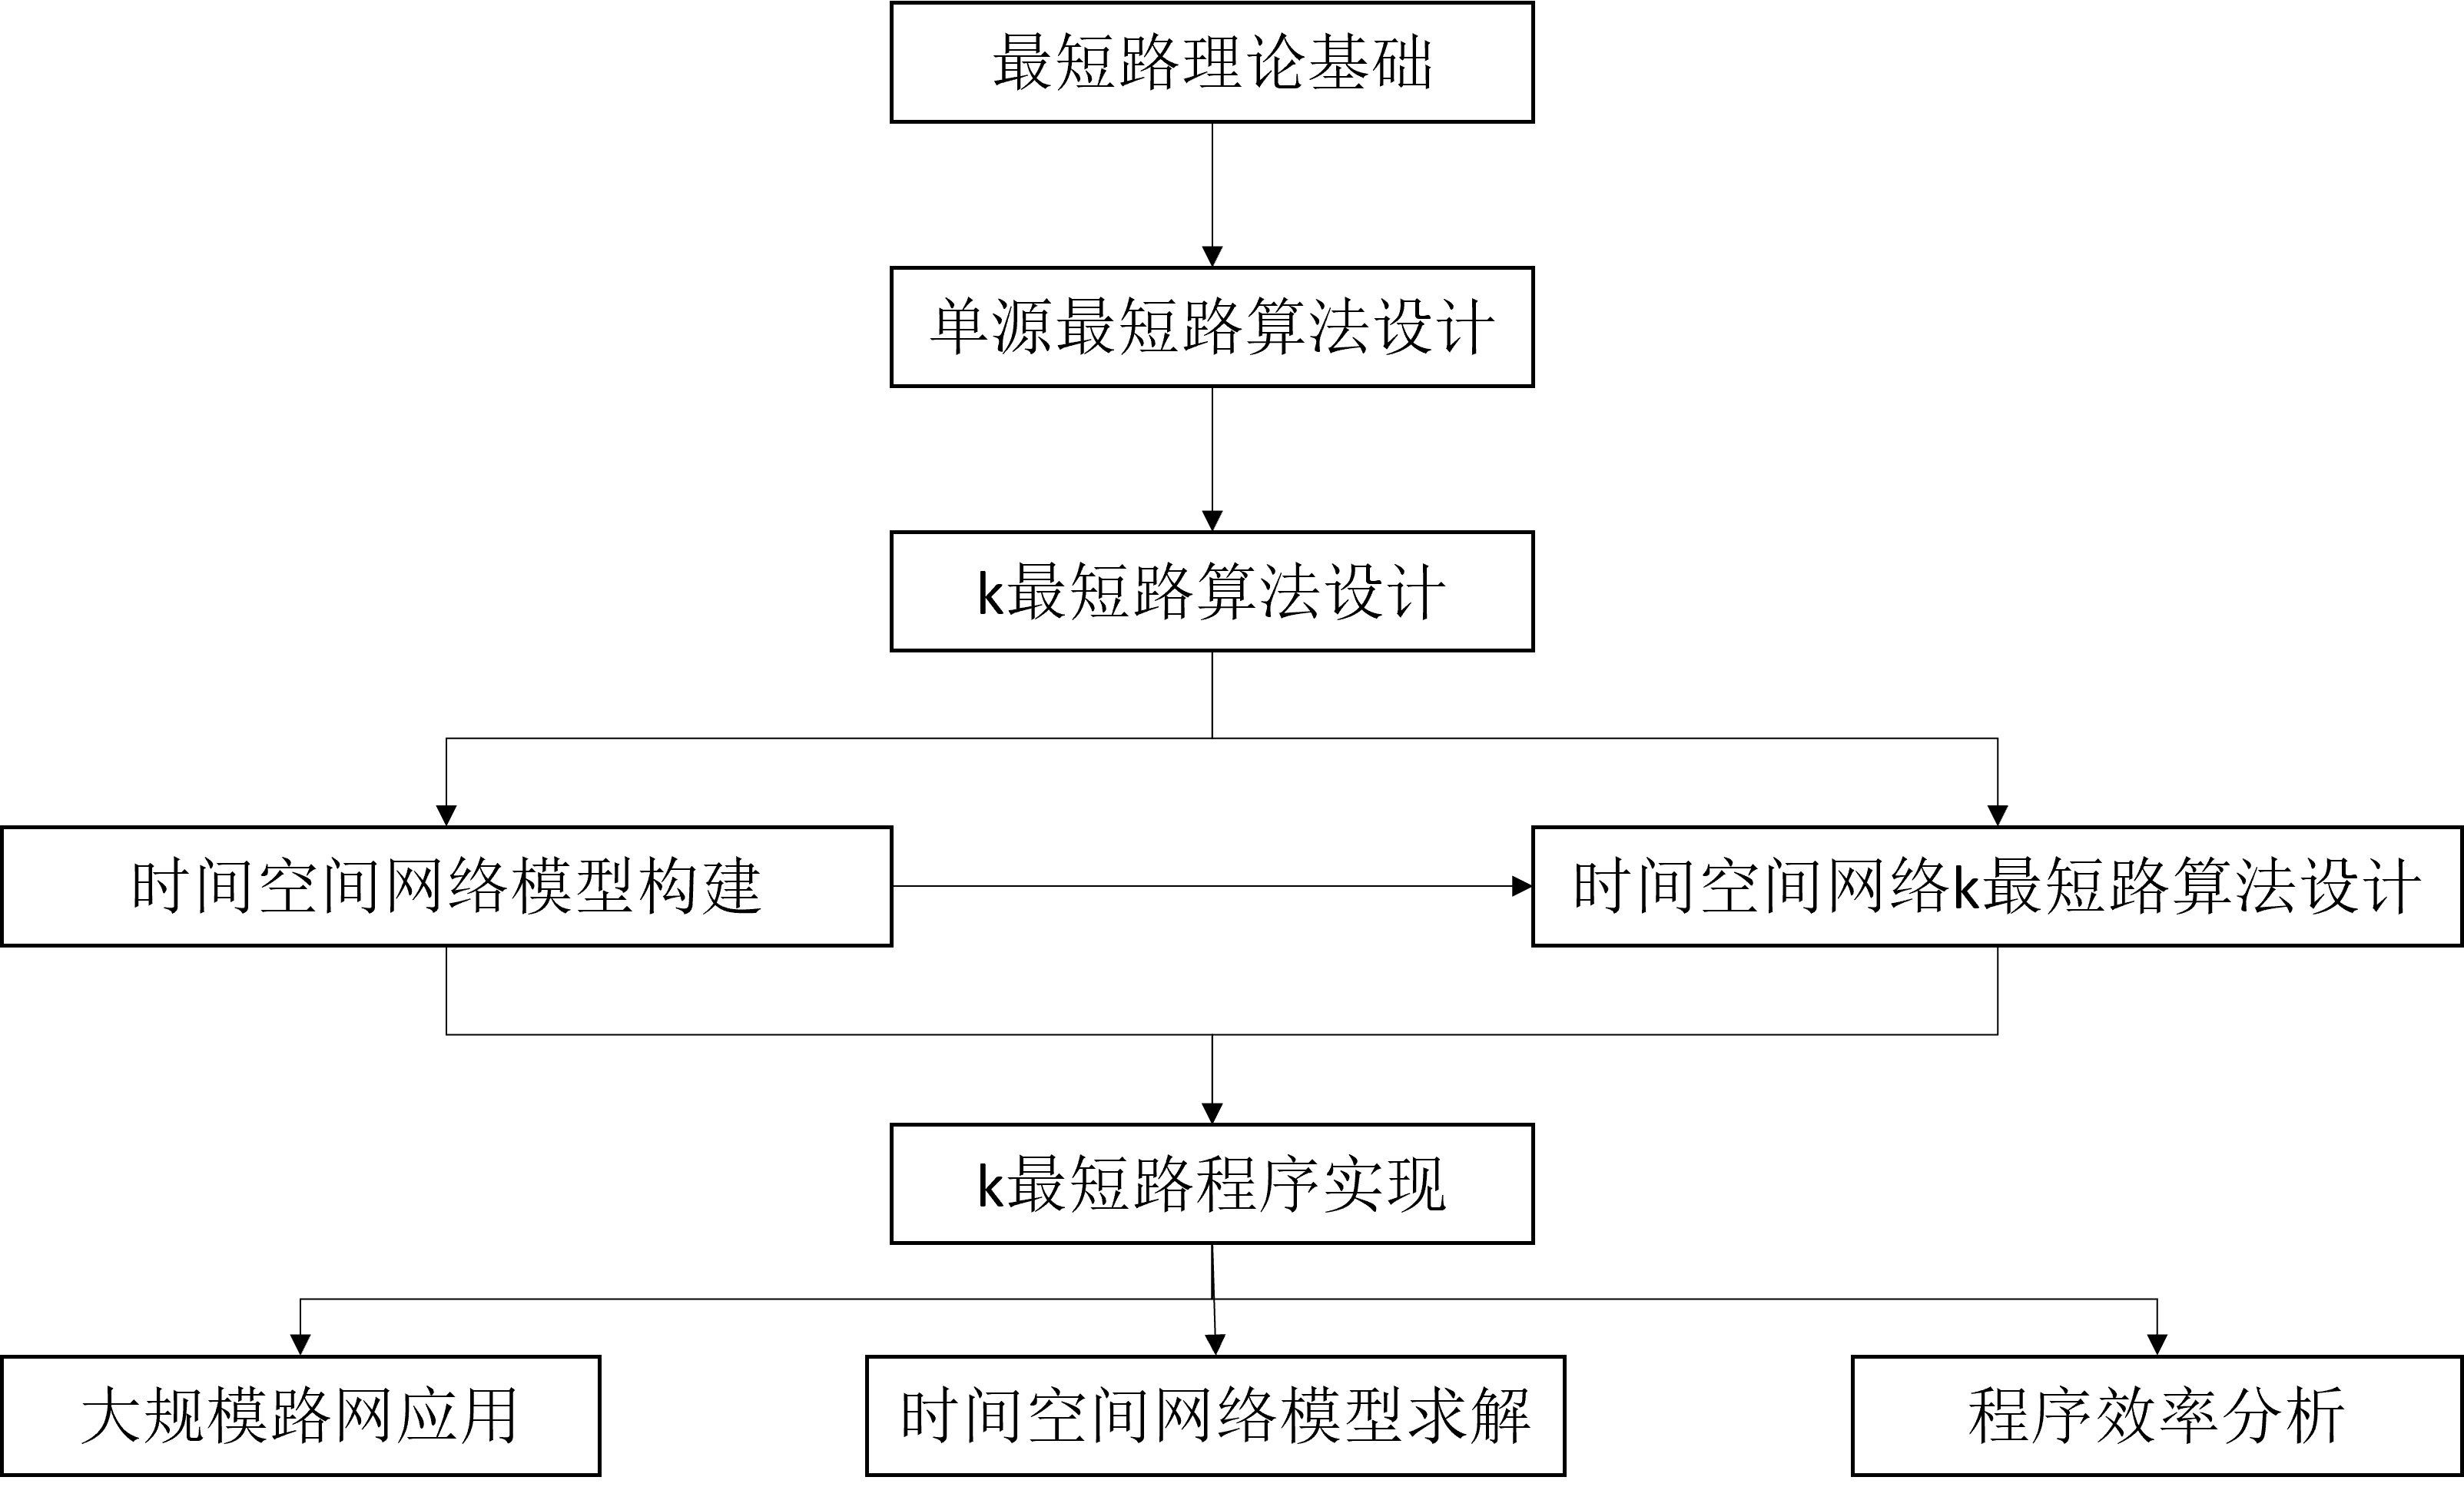
\includegraphics[width=0.7\textwidth]{png/图片1 研究技术路线图} %插入图片,[]中设置图片大小,{}中是图片文件名
    \caption{研究技术路线图} %最终文档中希望显示的图片标题
    \label{fig:fig1} %用于文内引用的标签
\end{figure}

\subsection{论文构成}\label{subsec:论文构成}
论文第1章主要介绍多条最短路在交通领域应用的研究背景和研究意义,目前国内外在相关领域的研究近况以及本文的主要研究内容。


论文第2章主要介绍图论中最短路理论基础,为后面的章节打下基础。


论文第3章结合交通领域的特点,对现有一般网络的拓扑结构进行拓展,并对时间-空间网络进行描述,以便在网络中反映出交通流动态变化的特点。


论文第4章对建立的时间-空间网络模型进行多条最短路算法的设计和求解。


论文第5章通过一个简单的网络案例进行模型的正确性和算法的有效性验证,并通过开源软件进行网络的可视化展示和可达性分析。


论文第6章通过开源平台构建城市交通道路网络并对构建的对象网络进行模拟。

%\nomenclature{PF}{powerful fingers}
%\nomenclature{KF}{kung fu}
    \let\cleardoublepage\clearpage


\chapter{最短路理论基础}\label{ch:最短路理论基础}
最短路问题与我们的日常生活息息相关,例如我们常常需要使用某种地图软件或者导航系统来获取从一个地方到另一个地方的路径。我们便可以得到对应该问题的图模型:以顶点对应交叉口,以边对应公路,边的权重对应经过该路段的成本,可以是时间、距离、偏好等等。


\section{符号定义}\label{sec:符号定义}
%center居中环境
\begin{center}
    %    tabular表格
    \begin{tabular}{l l}%    c表示居中, l表示左对齐, r表示右对齐
        \hline
        符号         & 含义                                       \\
        \hline%hline表示水平分割线, 使用|表示垂直分割线
        $G(V,E,W)$ & 网络                                       \\
        $N$        & 图中顶点的数量                                  \\
        $M$        & 图中边(弧)的数量                                \\
        $s$        & 最短路的源点                                   \\
        $t$        & 最短路的汇点                                   \\
        $D(u)$     & 从源点$s$到节点$u$的实际最短路距离                     \\
        $dis(u)$   & 从源点$s$到节点$u$的预测最短路距离                     \\
        $w(u,v)$   & 边的权重                                     \\
        $S$        & 已确定最短路径长度的节点的集合                          \\
        $T$        & 未确定最短路径长度的节点的集合                          \\
        $(i)$      & 表示图中的第$i$个节点,$i$的范围从$1$到$n$              \\
        $d_{ij}$   & 表示节点(i)到节点(j)之间的路段距离                     \\
        $A^k$      & 表示从$(1)$到$(n)$的第$k$条最短路径                 \\
        $A^k_i$    & 表示第$k-1$条最短路$A^{k-1}$上的第$i$个结点为偏离点时的偏离路径 \\
        $(R^k)_i$  & 源点到偏离点的距离长度                              \\
        $S^k_i$    & 偏离点到汇点的距离长度                              \\
        \hline
    \end{tabular}
\end{center}


\section{相关概念}\label{sec:相关概念}
\begin{itemize}%无序列表
    \item \textbf{距离约束条件}\\对于网络中的任意一条路径,均满足$dis(u)\geq D(u)$,当且仅当当前路径对应实际的最短路时等号成立
    \item \textbf{偏离点}\\偏离点表示最短路径和偏离路径$A^k$和$A^{k-1}$的前$i-1$个结点相同,在第$i$个结点处发生偏离, 其中第$k$条最短路径中的第$i$个结点到第$i+1$个结点的边, 即$(i)^k \to (i+1)^k$不能和现有的前$k-1$条最短路$A^j$中的边重复,其中$j$的范围从$1$到$k-1$
    \item \textbf{偏离路径}\\表示第$k-1$条最短路$A^{k-1}$上的第$i$个结点为偏离点时的偏离路径,$i$的范围从$1$到$Q_k$,其中$Q_k$表示第$k-1$条最短路径中的结点数量-1(不包括汇点),且不能在汇点处偏离。
    \item \textbf{根路径}\\表示第$k$条最短路径和第$k-1$条最短路径在结点$i$之前相同的路径
    \item \textbf{偏离距离}\\表示偏离路径$A^k$中第$i$个结点到汇点的距离,即$(i)\to\dots\to(n)$的距离
    \item \textbf{偏离路径距离}\\偏离距离与根距离之和
    \item \textbf{邻接矩阵}\\邻接矩阵是表示顶点之间相邻关系的矩阵。对于无向图而言,邻接矩阵是一个对称图,根据路径权重,一般将主对角线上的元素的路径阻抗设置为-1,表示不存在自环的回路。对于副对角线上的元素则不能唯一确定,且由于无向图中的邻接矩阵是对称矩阵,所以对于大规模的邻接矩阵会存在大量的冗余数据,因此可以使用压缩存储的方法来节省存储空间,提高存储效率和检索效率。对于有n个节点的图,如果使用邻接矩阵存储,则需要$n^2$的存储空间。
    \item \textbf{邻接表}\\邻接表是图论中用于描述一种相邻关系的数据结构。邻接表这种数据结构的优点是存储效率高,对于相邻边的检索效率高,可以使用出边表和入边表快速查找到某个节点的全部信息。邻接表美中不足的地方在于无法明确在什么地方保存相关边的长度或保存该长度所需要的额外代价。在一个邻接表中,给定任意一个顶点,可以在O(1)的时间内找到该顶点的出边和入边,而在邻接矩阵中需要花费O(n)的时间,而在最短路径算法中常常需要使用到出边和入边,因此使用邻接表对于实现最短路径算法的效率会更高。
    \item \textbf{稀疏图}\\如果网络中路径的个数远远小于其节点的平方,则称为稀疏图,而当网络中的路径个数接近其节点数的平方时,则称为稠密图。一般情况下,稀疏图使用邻接表进行存储,稠密图选择邻接矩阵进行存储。交通网络作为一种典型的稀疏图,因此之后对交通网络的存储会选择使用邻接表的方式进行存储,而对于动态的交通网络,将会通过对邻接表的表示方法进行拓展从而完成动态交通网络的存储。
    \item \textbf{有向图}\\对于图中的每一条边(u,v),若不仅表示结点u和结点v直接相连,同时表示方向,则称为有向图。其中节点u称为边的起点,节点v称为边的终点,同时节点u称为节点v的直接前驱,节点v称为节点u的直接后继。而无向图则仅仅表示结点u和结点v的连接性,所以可以通过两条有向边u`->`v,v`->`u进行表示,因此有向图的表达能力更强,适用于两个方向交通条件存在差异的网络建模中。
    \item \textbf{邻域}\\若结点u和结点v分别是边e的起点和终点,则称结点u和结点v是相邻的,称结点u(或者结点v)和边e是关联的。结点u的领域由与结点u关联的边e的关联结点v组成的集合,记为N(u)。
    \item \textbf{简单图}\\若一个图中没有单个结点构成的自回路,同时任意两个相邻结点的某一方向上至多仅有一条边,那么这样的图称为简单图。在后面的讨论中,对网络的建模将默认为简单图。
    \item \textbf{度}\\图中和一个顶点相关联的边的数量称为顶点的度数。度可以分为出度和入度,由于对图的存储必须包括对顶点的存储和对顶点关系的存储,因此图的邻接表存储方法是一种空间利用率最高的方法。在一般的需求中,往往只需要存储结点的出度或入度,但是对于速度要求较高的场景下,也可以以空间换时间的方法来同时存储图的出度表和入度表,例如A-star算法中建立反向图时则需要使用到结点的入度表。
    \item \textbf{正权图}\\若图G(V,E)的每条边e=(u,v)都被赋予一个数值作为该条边的权重,则将该图G称为加权图。如果每条边的权重数值都是一个非负实数,则称该图为正权图,例如经典的最短路算法Dijkstra算法要求图为正权图。
    \item \textbf{路径}\\途径是指由网络中若干个节点前后连接起来的边的集合。这个边集相邻边满足前一条边的终点为后一条边的起点,因此途径可以简写为$v_0\to v_1\to \dots \to v_n$,其中n称为途径的长度。若对于一条途径中任意两条边都不相同,则称该途径为迹。对于一条迹,若其中任意两个节点都不相同,则称成路径或简单路径。在交通领域中,所求的最短路径默认为不存在两次经过重复的节点,即路径中不存在环路。
    \item \textbf{反向图}\\在原有的有向图的基础上,对于每一条表示u$\to$v路段的有向边(u,v),通过建立一条与之权重相同,方向相反的有向边(v,u)来表示v$\to$u。反向图在最短路算法中的A-star算法中有着相当重要的作用,可以通过预处理来获取到当前节点到目标节点的预计最短路代价,同时也可以执行双向搜索算法,从而加快最短路算法的搜索效率。
\end{itemize}


\section{松弛操作}\label{sec:松弛操作}
对于某条特定的边(u,v),可以通过公式进行松弛操作:
\begin{equation}
    dis(v) = \min(dis(v),dis(u)+w(u,v))\label{eq:equation}
\end{equation}
松弛操作是一种典型的动态规划,其具体含义为:对于任意一条边,其状态只有两种情况,(a)处于最短路径中,(b)不处于最短路径中;
如果边(u,v)处于最短路径中,则表明从源点s到节点v的最短距离必定等于从源点s到节点u的最短距离加上边(u,v)的权值,即满足
\begin{equation}
    D(v) = D(u) + w(u,v)\label{eq:equation2}
\end{equation}

松弛操作的本质是判断一个顶点是否有更好的选择路径,如果已知的最短路径已经是实际上的最短路径,则不能找到一个额外的结点来使得上述公式成立。
描述松弛一般是指对边的松弛,在实际的操作过程往往使用对顶点进行松弛操作。所谓的对顶点进行松弛,便是对一个顶点的所有出边进行松弛操作。


\section{拉格朗日乘子法}\label{sec:拉格朗日乘子法}
拉格朗日乘子法作为一种优化算法,拉格朗日乘子法主要用于解决约束优化问题,它的基本思想就是通过引入拉格朗日乘子来将含有n个变量和k个约束条件的约束优化问题转化为含有(n+k)个变量的无约束优化问题。
拉格朗日乘子背后的数学意义是其为约束方程梯度线性组合中每个向量的系数。

如何将一个含有n个变量和k个约束条件的约束优化问题转化为含有(n+k)个变量的无约束优化问题?
拉格朗日乘数法从数学意义入手,通过引入拉格朗日乘子建立极值条件,对n个变量分别求偏导对应了n个方程,然后加上k个约束条件(对应k个拉格朗日乘子)一起构成包含了(n+k)变量的(n+k)个方程的方程组问题,这样就能根据求方程组的方法对其进行求解。

拉格朗日乘子法除了可以解决等式约束外,还可以解决不等式约束。大多数情况下等式约束不足以描述实际问题,因此拉格朗日乘数法在引入KKT条件之后可以用来处理不等式约束问题。KKT条件是指在满足一些有规则的条件下, 一个非线性规划(Nonlinear Programming)问题能有最优化解法的一个必要和充分条件。
这是一个广义化拉格朗日乘数的成果。一般地, 一个最优化数学模型的列标准形式参考开头的式子, 所谓 Karush-Kuhn-Tucker 最优化条件,就是指上式的最优点$x^*$必须满足下面的条件:
\begin{equation}
    \left.
    \begin{array}  { l  }
    { L ( x , u ) = f ( x ) + \sum _ { k = 1 } ^ { a } u _ { k } g _ { k } ( x ) }
        \\ { \quad u _ { k } (x) \geq 0 }
        \\ { g _ { k } ( x ) \leq 0 }
    \end{array}
    \right.\label{eq:equation3}
\end{equation}

KKT条件是拉格朗日乘子法的泛化,再引入了等式约束和不等式约束后,可以将原问题转为化对偶问题进行求解,当满足一定条件时,对偶问题的解和原问题的解是相同的。此时可以将问题转化为
\begin{equation}
    \min_{x}\max _{\mu}L(x, \mu)= \max _{\mu}\min m_{x}L(x, \mu)= \min _{k}f(x)=f(x^{*})\label{eq:equation4}
\end{equation}
    \chapter{时间-空间网络的构建与拓展表示}\label{ch:时间-空间网络的构建与拓展表示}

在传统的网络问题上,路段上的路段阻抗常被视作是一个常数,也称为静态路网。而对于现实情况的交通路网,路段阻抗函数通常受到多重影响因素的共同作用,需要考虑随机性和时变性等问题,因此路段阻抗函数应该为时间的函数,即d=f(t)。并且在动态网络中,各路段和相关节点之间是相互作用的,在网络中某个节点或路段发生故障,其造成的影响不仅仅是该条路段或该节点,而是一个区域的路段和节点。

为了刻画交通网络的动态性和网络中路段和节点之间的相关作用关系,本章节将主要对比地介绍一般的物理交通网络表示和离散的动态交通网络的时间-空间表示以及对网络拓扑结构中节点和路段关系约束的拓展表示。


\section{物理交通网络表示}\label{sec:物理交通网络表示}

在交通运输规划和管理领域中,物理交通网络一般表示为有向图G=(V, E, W) 。其中$V=\{1, 2, \dots,n\}$表示网络中节点的集合,
而$E=\{(i,j) \in V \times V\}$表示边的集合,其中(i,j)表示从节点i到节点j的有向路段。路段的数量用m表示,使用$W=\{w_{ij} (t)|(i,j)\in E\}$表示随时间变化的路段行程时间集合。
在如图\ref{fig:fig2}所示的交通网络中,有6个节点和13条路段,每条路段都有相对应的权重,即表示路段行程时间。
\begin{figure}[H] %H为当前位置,!htb为忽略美学标准,htbp为浮动图形
    \centering %图片居中
    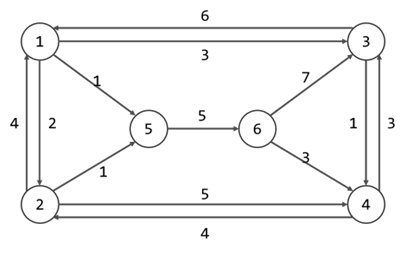
\includegraphics[width=0.7\textwidth]{png/图片2 简单静态交通网络示例} %插入图片,[]中设置图片大小,{}中是图片文件名
    \caption{简单静态交通网络示例} %最终文档中希望显示的图片标题
    \label{fig:fig2} %用于文内引用的标签
\end{figure}

对于静态网络,经典的最短路算法可以很高效的计算出网络中的最优路径。
然而对于动态网络,例如动态随机网络则不能很好的求解,
如图\ref{fig:fig3}所示。驾驶者从节点1处出发,可以经过路径A:$1 \to 3 \to 6$或路径B:$1\to 2\to 3\to 6$这两条路径到达节点6。
由于两条路径中到达节点3的到达时间不相同,即两条路径中$3\to 6$的出发时间不相同,因此对于同一路段产生了不同的路段行程时间。
\begin{figure}[H] %H为当前位置,!htb为忽略美学标准,htbp为浮动图形
    \centering %图片居中
    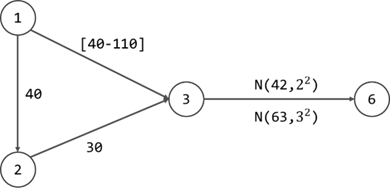
\includegraphics[width=0.7\textwidth]{png/图片3 动态随机网络} %插入图片,[]中设置图片大小,{}中是图片文件名
    \caption{动态随机交通网络示例} %最终文档中希望显示的图片标题
    \label{fig:fig3} %用于文内引用的标签
\end{figure}

假设一个具体的场景:驾驶者在7:00从节点1出发,路段$1 \to 3$的行程时间服从U(40,110)的均匀分布,
而路段$1\to 2\to 3$的总行程时间为固定的40+30=70,假设在节点内部同样存在时间的消耗,例如8:00---8:30节点3处的行程时间消耗为7,
而在其他时间行程时间消耗为1,在8:15之前出发的情况下,路段(3,6)的路段形成时间服从正态分布$N(63,3^2)$,
而8:15之后出发的话路段服从正态分布$N(42,2^2)$。对于路径13的期望最短行程时间为75,
而路径$1\to 2\to 3$的最短行程时间为70,但是$1\to 3\to 6$的期望最短行程时间为124,而$1\to 2\to 3\to 6$的期望最短行程时间为140。
可以看出,动态最短路问题已经不满足Bellman条件:每条最短路径的子路径也是最短路径,即若节点i到节点j的最短路径中经过节点k,
则节点i到节点k的最短路径是节点i到节点j的最短路径的前缀。同样,Bellman条件也不适用于时间-空间网络中最短路的求解。


\section{时间-空间交通网络表示}\label{sec:时间-空间交通网络表示}
与上面介绍的静态交通网络相比,时间-空间网络能够更好地描述出现实世界中交通网络的动态变化性质,
例如在一天早晚高峰时段路段的阻抗会呈现出双峰分布,而在相邻的时间段内路段阻抗值差异较小,
如图\ref{fig:fig4}所示。由于交通流具有明显的周期性,通常来说可以以一天或一周为一个周期进行分析,
对于路段的阻抗信息,可以根据该区域内路段的历史阻抗信息,
采用时间序列分析的方法来预测将来相应时间段内的路段阻抗。

\begin{figure}[H] %H为当前位置,!htb为忽略美学标准,htbp为浮动图形
    \centering %图片居中
    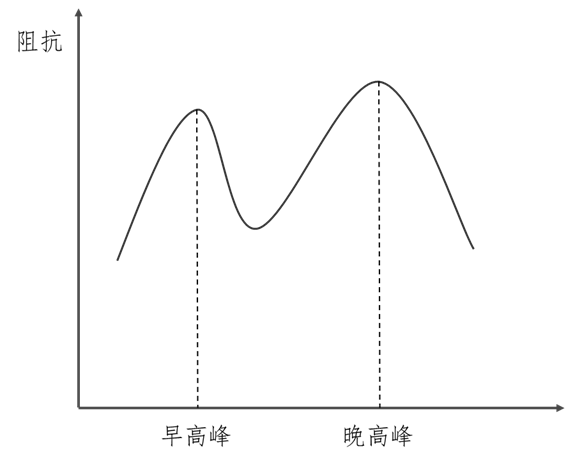
\includegraphics[width=0.7\textwidth]{png/图片4 路段阻抗分布} %插入图片,[]中设置图片大小,{}中是图片文件名
    \caption{路段阻抗分布} %最终文档中希望显示的图片标题
    \label{fig:fig4} %用于文内引用的标签
\end{figure}

时间-空间网络表示可以根据阻抗函数和时间的函数关系分为连续网络和离散网络,
根据前面对交通流的分析,交通网络中在一定时间内的路段阻抗值相差不大,
因此接下来将使用离散时间-空间网络建模,同时离散网络也对问题作出一定程度的简化且方便计算机求解,
可以使得动态网络转变为相对应的静态网络进行求解,对路段阻抗离散化处理之后的结果如图\ref{fig:fig5}所示。

\begin{figure}[H] %H为当前位置,!htb为忽略美学标准,htbp为浮动图形
    \centering %图片居中
    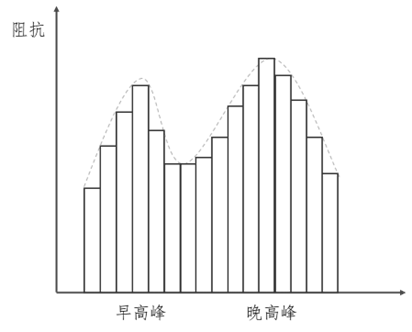
\includegraphics[width=0.7\textwidth]{png/图片5 路段阻抗离散化处理结果} %插入图片,[]中设置图片大小,{}中是图片文件名
    \caption{路段阻抗离散化处理结果} %最终文档中希望显示的图片标题
    \label{fig:fig5} %用于文内引用的标签
\end{figure}

上面已经对单条路段的阻抗函数进行了离散化处理,
而对于时间-空间路网则需要对路网中所有的路段进行离散化处理,
常用形式有时间拓展图和时间集聚图。时间聚集图通过一个序列来表示路段上的阻抗,
占用的内存相比于时间拓展图而言更少,因此对于规模相对较大的网络而言处理速度更快,效率更高。

\begin{figure}[H] %H为当前位置,!htb为忽略美学标准,htbp为浮动图形
    \centering %图片居中
    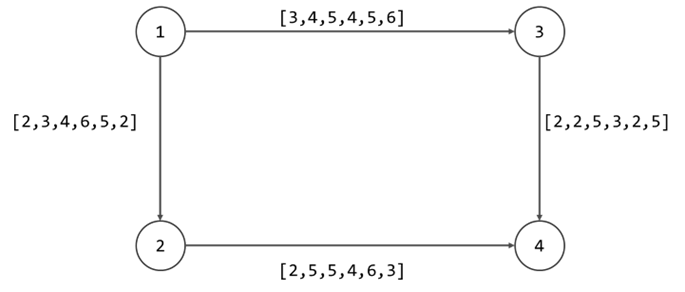
\includegraphics[width=0.7\textwidth]{png/图片6 时间聚集图} %插入图片,[]中设置图片大小,{}中是图片文件名
    \caption{时间聚集图} %最终文档中希望显示的图片标题
    \label{fig:fig6} %用于文内引用的标签
\end{figure}
在如图\ref{fig:fig6}所示的时间聚集图中,将每条路段的阻抗划分为6个切片,
分别代表6个不同时段的路段阻抗值。时间聚集图虽然可以相对高效的求解网络最短路,
但是不如时间拓展图直观,网络实际拓扑结构也不清晰。
若将图\ref{fig:fig6}所示的时间聚集图展开为时间拓展图, 则如图\ref{fig:fig7}所示。
时间拓展图会使得原本简单的网络拓扑变得异常复杂,网络中节点的数目根据切片数量成倍数增长,
即$N=kN_0$,其中$N_0$是时间拓展图中节点的数量,k为切片数量,N为时间拓展图中节点的数量。

\begin{figure}[H] %H为当前位置,!htb为忽略美学标准,htbp为浮动图形
    \centering %图片居中
    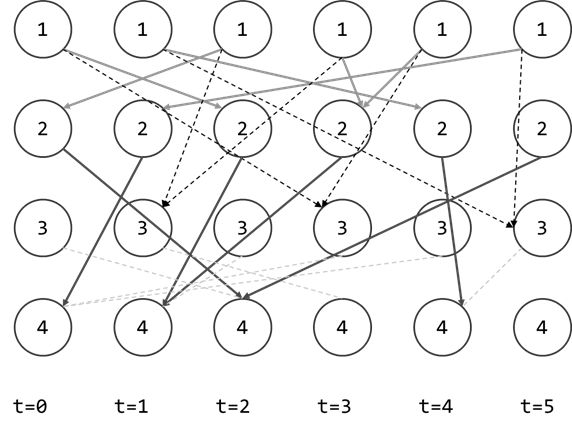
\includegraphics[width=0.7\textwidth]{png/图片7 时间拓展图} %插入图片,[]中设置图片大小,{}中是图片文件名
    \caption{时间拓展图} %最终文档中希望显示的图片标题
    \label{fig:fig7} %用于文内引用的标签
\end{figure}

对于考虑从任意时间,任意节点出发的一个网络,将出发时刻视作t=0,出发节点视作节点1,
此时可以将时间拓展图简化为时间-空间交通网络状态图,如图\ref{fig:fig8}所示。
时间-空间状态相比于时间拓展图的存储效率更高,适用于路段交通流量差异较大的实时计算中使用。

\begin{figure}[H] %H为当前位置,!htb为忽略美学标准,htbp为浮动图形
    \centering %图片居中
    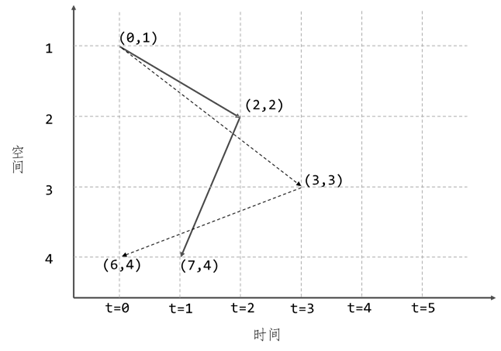
\includegraphics[width=0.7\textwidth]{png/图片8 时间-空间状态图} %插入图片,[]中设置图片大小,{}中是图片文件名
    \caption{时间-空间状态图} %最终文档中希望显示的图片标题
    \label{fig:fig8} %用于文内引用的标签
\end{figure}
同时,一条实际的物理路径可能对应时间-空间交通网络中的多条不同时刻出发和不同时刻到达的路径。
如图\ref{fig:fig8}所示,从节点1到节点4仅在t=0时刻便分别对应$1\to 2\to 4$和$1\to 3\to 4$两条路径。
因此对所研究的问题,我们可以在传统的静态最短路网的基础上,
针对驾驶者的出发时刻和出行决策建立动态的最短路模型,具体建模过程将于第四章进行具体介绍。


\section{交通网络节点拓扑结构的拓展表示}\label{sec:交通网络节点拓扑结构的拓展表示}
在上面的时间-空间网络中,我们已经可以在构建的模型中很好地体现出交通网络的动态性和周期性,
但是却没有考虑到节点阻抗造成的影响。在很多场景下,节点阻抗对网络路径造成的影响是不可忽略的,
例如在交叉口左转、右转、直行,又或者在不同的地铁线路之间换乘,
因此我们需要通过一定的方法将节点阻抗转变为路段阻抗,从而完成对问题形式上的统一,
方便对问题进行求解。下面以图\ref{fig:fig9}所示南京地铁线路图为例,介绍如何在交通网络的拓扑结构中对节点阻抗进行描述。

\begin{figure}[H] %H为当前位置,!htb为忽略美学标准,htbp为浮动图形
    \centering %图片居中
    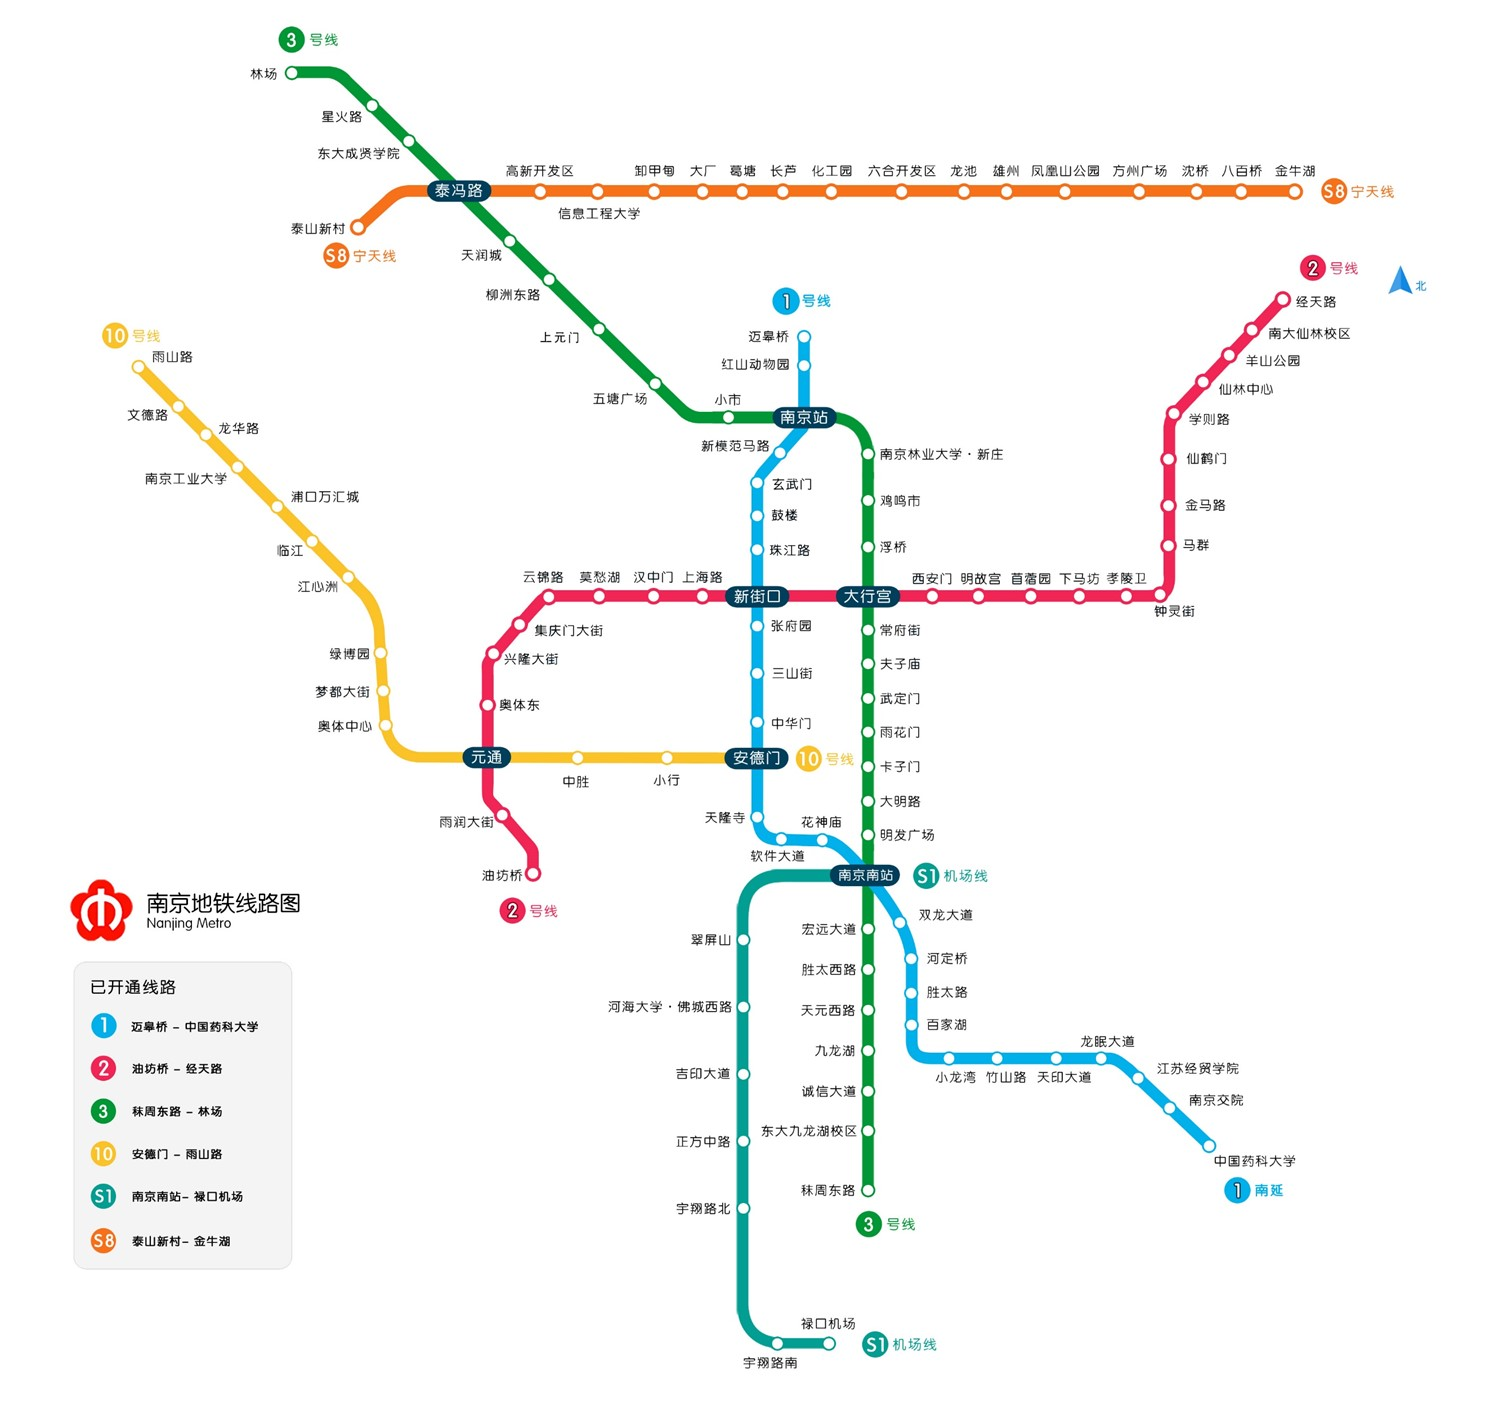
\includegraphics[width=0.7\textwidth]{png/图片9 南京地铁线路图} %插入图片,[]中设置图片大小,{}中是图片文件名
    \caption{南京地铁线路图} %最终文档中希望显示的图片标题
    \label{fig:fig9} %用于文内引用的标签
\end{figure}

以地铁1号线和地铁3号线的换乘站(南京南站)为例,
上面所述的时间-空间网络状态图中在南京南站乘客换乘的时间没有考虑,
因此需要对节点进行拓展,采用拆点法的思想,将节点拆分为多对出发节点和到达节点,
在换乘线路之间添加惩罚项,而没有换乘行为的路段则认为对应一条阻抗值为0的路段,如图\ref{fig:fig10}所示。

\begin{figure}[H] %H为当前位置,!htb为忽略美学标准,htbp为浮动图形
    \centering %图片居中
    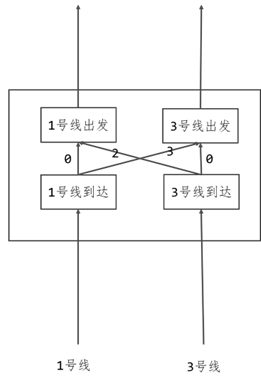
\includegraphics[width=0.5\textwidth]{png/图片10 换乘站结点的拓展表示} %插入图片,[]中设置图片大小,{}中是图片文件名
    \caption{换乘站结点的拓展表示} %最终文档中希望显示的图片标题
    \label{fig:fig10} %用于文内引用的标签
\end{figure}

综上所述,在时间-空间网络结合交通网络有着自己独特的流量特点,时间-空间交通网络呈现周期性的变化特点,且在微观上交通流的变化是连续的,而在宏观上交通流的变化是离散的,呈现出双峰分布的特点。
因此时间空间网络中的多条最短路问题可以通过时间拓展图的处理方法转化为静态网络中多个源点序列到多个汇点序列的多条最短路问题。
时间-空间拓展网络如图\ref{fig:fig11}所示。

\begin{figure}[H] %H为当前位置,!htb为忽略美学标准,htbp为浮动图形
    \centering %图片居中
    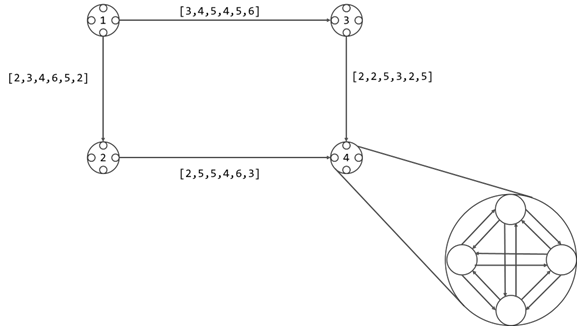
\includegraphics[width=0.7\textwidth]{png/图片11 节点拓展的时间-空间网络状态图} %插入图片,[]中设置图片大小,{}中是图片文件名
    \caption{节点拓展的时间-空间网络状态图} %最终文档中希望显示的图片标题
    \label{fig:fig11} %用于文内引用的标签
\end{figure}
    \chapter{时间-空间网络中多条最短路算法设计}\label{ch:时间-空间网络中多条最短路算法设计}
多条最短路有两个核心特点: 一个是多,一个最短。首先,最短路算法是智能交通系统的核心。
在构建城市智能交通系统中,最重要的就是选择最优的路径规划算法,实现在复杂的城市路网中找出最适合用户的路径其次,最短也有多层含义,根据不同驾驶者的需求差异,或要求距离最短,或要求时间最短,或要求可靠性高。
同时,在具体的出行方式中可能还有各种细分的出行需求,例如在选择地铁出行方式中,可能还有换乘最少等需求;
在选择公交出行方式中,可能有步行最少等需求。
此外,即使是同一驾驶者,在不同的时间节点的出行需求很大可能是不同的,
例如在上班途中,一般来说都是尽可能选择最短时间,最短距离的路径从而快速到达公司,避免迟到。
而在下班途中,即使绕道,可能也需要去某些大型连锁超市购买晚餐的食材。
多条最短路可以避免因网络中路段的故障,例如路段施工维护等原因造成目的地不可达,提高了路径选择算法的容错性和ITS的可靠性。
综上所述,多条最短路一能提供最为经济或效率最高的出行方式。
二能根据用户的差异性需求提供个性化的路径导航。
三能提高系统的可靠性。
所以说,多条最短路问题的研究对人们的日常生活用着极大的影响。

时间-空间交通网络属于动态网络,而动态网络中的最短路径的求解依赖于静态网络中最短路的基础,而k条最短路问题属于最短路径问题的变体。
因此接下来我们将首先研究静态网络中的最短路算法设计,再研究静态网络中的k条最短路算法的设计,
最后根据第三章对时间-空间网络模型的表示方法,将时间-空间网络中k条最短路问题转化为一个时间拓展图中的k条最短路问题,从而实现对动态网络中k条最短路算法的设计。


\section{单源最短路算法设计}\label{sec:单源最短路算法设计}
有很多算法在图形上运行。本文将主要介绍广度优先搜索,Dijkstra算法和A-star算法。

广度优先搜索在所有方向上都进行了同等的探索。这是一个非常有用的算法,不仅适用于常规路径查找,还适用于程序地图生成、流场路径查找、距离地图和其他类型的地图分析。

Dijkstra的算法(也称为统一成本搜索)让我们可以优先选择要探索的路径。与其平等地探索所有可能的路径,它更倾向于低成本的路径。我们可以分配更低的成本来鼓励在道路上移动,更高的成本来避免形成搜索森林,更高的成本来阻止接近敌人,等等。当移动成本发生变化时,我们使用这种方法,而不是广度优先搜索。

A-star是对Dijkstra算法的修改,该算法针对单个目的地进行了优化。Dijkstra算法可以找到所有位置的路径;A-star查找到一个位置或几个位置中最近位置的路径。它优先考虑那些似乎更接近目标的路径。

\subsection*{Dijkstra算法}
Dijkstra算法首先将全部节点集合分为两个集合:S集合和T集合。其中S集合表示已确定最短路径长度的节点的集合,而T集合表示未确定最短路径长度的节点的集合。
算法初始化时网络中的所有结点均属于T集合,首先将除源点s外其它所有点的距离初始值为无穷大,不断重复执行从T集合中取出到源点s具有最短路径的结点q,将其加入到集合S中,并对结点q的出边执行松弛操作直至集合S中包含网络中的全部节点


\begin{algorithm}
    \caption{Dijkstra算法}
    \begin{algorithmic}[1]
        \STATE 初始化: $S = \{s\}, T = U - S, dis(s)=0, dis(u)=+\infty$
        \REPEAT
        \STATE 取$q=\min(dis(u)), u \in T$
        \STATE $T.pop(u), S.push(u)$
        \STATE relax(u)
        \UNTIL S.length == N
        \STATE 算法结束
    \end{algorithmic}\label{alg:algorithm}
\end{algorithm}

\subsection*{A-star算法}
在导航系统中,我们经常需要找到从一个位置到另一个位置的可行路径,在更好的情况下,我们努力寻找系统中的最短路径,可能需要考虑到旅行时间,距离等。
为了找到这条路径,我们可以使用图形搜索算法A-star算法,A-star算法作为一种启发式算法,是图形搜索算法的常用选择。一般情况下,A-star算法以Dijkstra算法作为基础来寻找估计距离,
Dijkstra算法可以很好地找到最短的路径,但它会浪费时间去探索那些没有可能是最短路的方向。贪婪的“最佳优先搜索”(Best First Search)朝着有希望的方向探索,但它可能找不到最短的路径。
A-star算法使用从开始的实际距离和估计到目标的距离,即f(n)=g(n)+h(n),其中f(n)表示总成本,g(n)表示从开始位置到当前位置已经花费的成本,而h(n)表示从当前位置到目标位置的预计成本。

A-star算法首先需要定义open表和close表,在open表中存放已知但还未访问过的节点,在close表中存放已经访问过的节点;
再定义估价函数或启发式函数h(n),用来度量剩余距离,一般使用Dijkstra算法进行计算;
算法初始化时把起始节点加入到open表中,重复执行下面的操作
\begin{enumerate}%有序列表
    \item 如果open表为空,则寻路失败,找不到达到终点的路径。
    \item 遍历open表,选择总成本最小的节点作为接下来要处理的节点,并把这个节点加入到close表中
    \item 处理该节点的所有邻接节点
    \begin{enumerate}%有序列表
        \item 如果邻接节点在close表中,表示邻接节点在之前已经访问过,忽略即可;
        \item 如果邻接节点不在open表中,则把邻接节点加入到open表中,并将当前节点设置为邻接节点的父节点,计算邻接节点的总成本
    \end{enumerate}
    \item 如果终点加入到open表中,此时说明已经找到最佳路径,而由起点到终点以及之前关联的父节点便构成了一条最优路径
\end{enumerate}

\begin{algorithm}
    \caption{A-star算法}
    \begin{algorithmic}[1]
        \STATE 初始化: open =$\{s\}$, close
        \STATE 定义启发式函数h(n)
        \STATE 计算估计距离f(n) = g(n) + h(n)
        \STATE open.length == 0, 不存在最短路, 算法结束
        \REPEAT
        \STATE 遍历open表, 选择f(n)最小的结点u
        \STATE open.pop(u), close.push(u)
        \STATE 寻找u的邻接节点v
        \STATE  open.push(v),
        \STATE  计算结点v的估计距离
        \UNTIL open.length == 0
        \STATE 算法结束
    \end{algorithmic}\label{alg:algorithm2}
\end{algorithm}


\section{多条最短路算法设计}\label{sec:多条最短路算法设计}
首先借助下面的简单路网说明以下偏离点和偏离路径的概念,
在图\ref{fig:fig12}中可以通过上面介绍的经典的单源最短路算法,
如Dijkstra算法或A*算法求得源点s到汇点t的最短路径p1为$s\to 1\to t$,
路径成本代价为1+3=4。
在k最短路径中,除汇点t之外路径上的其它节点,
都被称为偏离点。而源点s到汇点t的次短路径p2为$s\to 1\to 2\to t$,路径成本为1+2+2=5,
此时路径p2相对于路径p1的偏离节点为节点1,即节点1为路径p1到路径p2的偏离点,
而路段$1\to 2\to t$被称为路径p1到路径p2的偏离路径。
\begin{figure}[H] %H为当前位置,!htb为忽略美学标准,htbp为浮动图形
    \centering %图片居中
    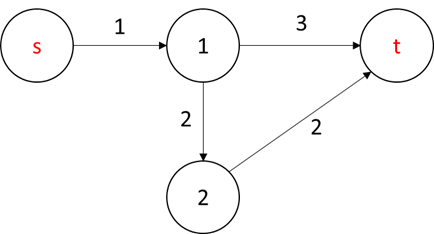
\includegraphics[width=0.7\textwidth]{png/图片12偏离点和偏离路径} %插入图片,[]中设置图片大小,{}中是图片文件名
    \caption{偏离点和偏离路径} %最终文档中希望显示的图片标题
    \label{fig:fig12} %用于文内引用的标签
\end{figure}

\subsection{设计思路}\label{subsec:设计思路}
该算法可以分为两个步骤,首先确定第一条最短的路径,即$A^1$,然后依次确定其他k-1条次短路径。
假定使用容器A来保存最短路径,而容器B将保存可能的k最短路径。
为了确定从起点到终点的k条最短路径,可以使用有效且高效的单源最短路径算法。

为了找到第k条最短路$A^k$,k的范围从2到K,
算法假设在寻找第k条最短路$A^k$之前已经发现了从$A^1$到$A^(k-1)$的所有路径。
因此第k轮迭代可以分为两个阶段:(a).找到所有的$A_i^k$;
(b).从所有的$A_i^k$中找出最短路径即为$A^k$。
在此迭代过程中,i的范围从1到$Q_k^k$。第一个过程可以进一步细分为三个操作,
(a).选择$R_i^k$,(b).寻找$S_i^k$,(c).将$A_i^k$添加到容器B中保存作为第k最短路的候选路径。

通过在上一次寻找到的最短路径$A^{k-1}$中一次选择除汇点之外的节点j作为偏离节点$A^j$,找到从源点到偏离节点的路径作为根路径$R^k_i$。
然后在偏离点容器中查找该偏离点出边所对应的路段,如果找到路径,则将相应路段的路段阻抗$d_{i(i+1)}$设置为无穷大。
接下来,通过偏离节点到汇点的最短路径找到偏离路径。确保偏离路径和偏离路径容器中的路径不同,添加根路径和偏离路径。
接下来,删除的路段(即将其成本设置为无限)恢复为初始值。
第二个过程通过在成本最低的容器中找到路径来确定合适的路径。该路径从容器中删除并插入容器中,该算法继续进行下一轮迭代。

\subsection{算法流程(伪代码描述)}\label{subsec:算法流程}
\begin{lstlisting}[label={lst:lstlisting7}]
function KSP(Graph, source, sink, K):
    // 首先通过Dijkstra算法初始化第一条最短路径
    A[0] = Dijkstra(Graph, source, sink);
    // 准备一个存放偏离路径的容器, 最为最短路径的备选路径
    B = [];
    // 通过迭代的方式, 依次顺序地计算出从第2条到第K条最短路径
    for k from 1 to K:
        for i from 0 to size(A[k − 1]) − 2:
            spurNode = A[k-1].node(i);
            rootPath = A[k-1].nodes(0, i);
            for each path p in A:
                if rootPath == p.nodes(0, i):
                    remove p.edge(i,i + 1) from Graph;
            for each node rootPathNode in rootPath:
                remove rootPathNode from Graph;
            spurPath = Dijkstra(Graph, spurNode, sink);
            totalPath = rootPath + spurPath;
            if (totalPath not in B):
                B.append(totalPath);
            restore edges to Graph;
            restore nodes in rootPath to Graph;
        if B is empty:
            break;
        // 排序, 获取当前轮次中所有可能是最短路径的偏离路径, 选择最短的路径
        B.sort();
        A[k] = B[0];
        // 选择最短的偏离路径, 并将其从容器中弹出
        B.pop();
    return A;
\end{lstlisting}


\section{时间-空间网络下的多条最短路算法设计}\label{sec:时间-空间网络下的多条最短路算法设计}
将输入的时间聚集图转换为方便计算机处理的时间拓展图
在时间拓展图中获得k条最短路, 原问题转化为6个起始节点到6个目标节点的最短路问题
算法缺点:
在计算机实际存储过程中, 时间空间网络会成倍消耗存储空间, 假设路段离散化序列的长度为k, 则存储的节点数是原来的k倍, 存储的路段数是原来的k^2倍
不适用于大规模网络, 因此对于大规模网络可能需要使用道路网络分层的思想

\subsection{模型存储结构设计}\label{subsec:模型存储结构设计}
在静态最短路算法中,我们只需要使用一个数字即可存储路段阻抗,因此可以使用邻接矩阵或者邻接表来存储静态网络。
一般来说,邻接矩阵适合存储稠密图,即$m\approx n^2$,
邻接表更适合存储稀疏图,即$m \ll n$。
而交通网络作为典型的一种稀疏图,所以选择邻接表进行存储,
例如对于图\ref{fig:fig2}所示的静态网络采用邻接表存储结果如图\ref{fig:fig13}所示。
\begin{figure}[H] %H为当前位置,!htb为忽略美学标准,htbp为浮动图形
    \centering %图片居中
    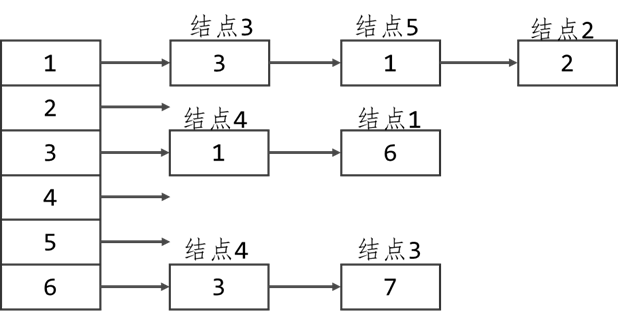
\includegraphics[width=0.7\textwidth]{png/图片13静态网络存储结构图} %插入图片,[]中设置图片大小,{}中是图片文件名
    \caption{静态网络存储结构图} %最终文档中希望显示的图片标题
    \label{fig:fig13} %用于文内引用的标签
\end{figure}

但在动态网络的最短路算法中,路段的阻抗是一个时间序列,
因此需要对上述的邻接表存储方式进行改进。之前的邻接表存储方式中,
一个结点只能存放一个值,现在需要一个结点中能够存放一个序列,
以图\ref{fig:fig6}所示的动态网络为例,对于动态交通网络的存储结构设计如图\ref{fig:fig14}所示。
\begin{figure}[H] %H为当前位置,!htb为忽略美学标准,htbp为浮动图形
    \centering %图片居中
    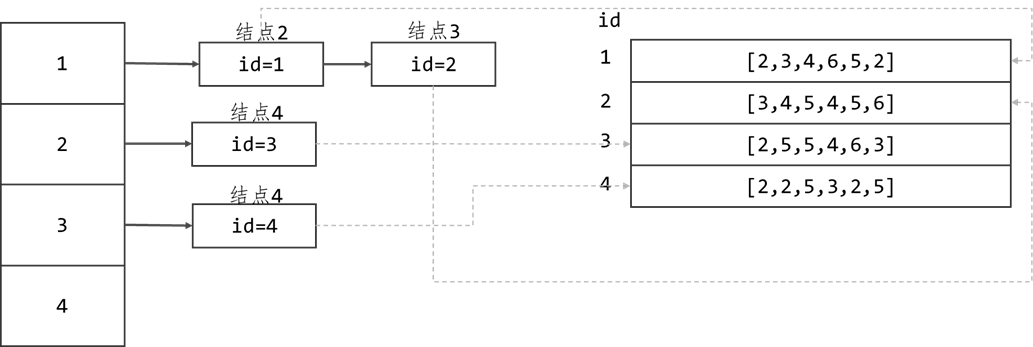
\includegraphics[width=0.7\textwidth]{png/图片14动态网络存储结构图} %插入图片,[]中设置图片大小,{}中是图片文件名
    \caption{动态网络存储结构图} %最终文档中希望显示的图片标题
    \label{fig:fig14} %用于文内引用的标签
\end{figure}

\subsection{模型求解}\label{subsec:模型求解}

\subsubsection{时间拓展图到静态网络的转化处理}
\begin{figure}[H] %H为当前位置,!htb为忽略美学标准,htbp为浮动图形
    \centering %图片居中
    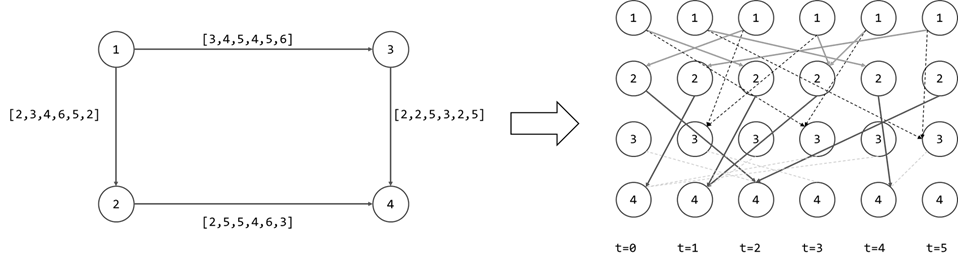
\includegraphics[width=0.7\textwidth]{png/图片15时间拓展图到静态网络的转化处理} %插入图片,[]中设置图片大小,{}中是图片文件名
    \caption{时间拓展图到静态网络的转化处理} %最终文档中希望显示的图片标题
    \label{fig:fig15} %用于文内引用的标签
\end{figure}
如图\ref{fig:fig15}所示,
根据时间拓展图中的时间序列的长度count=6,
可以将原本的时间拓展图表示为静态网络,
时间拓展图与静态网络等价的充分必要条件是满足路段阻抗和出发时刻之间的约束关系。
对于在时间拓展图中k时刻出发的任意节点from到目的节点to的约束条件
可以转化为静态网络中从出发节点(from*count + k)到目的节点(to*count+(k+cost)\%count)的一条约束,路段阻抗值保持不变。

\subsubsection{问题的等价转化}
\begin{figure}[H] %H为当前位置,!htb为忽略美学标准,htbp为浮动图形
    \centering %图片居中
    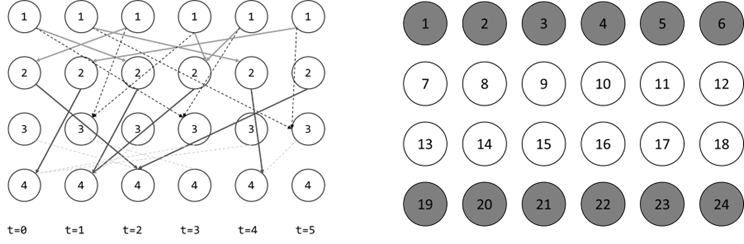
\includegraphics[width=0.7\textwidth]{png/图片16时间空间网络中k最短路问题的等价转化处理} %插入图片,[]中设置图片大小,{}中是图片文件名
    \caption{时间空间网络中k最短路问题的等价转化处理} %最终文档中希望显示的图片标题
    \label{fig:fig16} %用于文内引用的标签
\end{figure}

如图\ref{fig:fig16}所示,在时间拓展图中求解k最短路问题被等价转化为从count=6个起始节点(分别表示不同时刻出发的同一个节点)到
6个目的节点(分别表示不同到达状态的同一个节点)的最短路问题。由于实际交通网络中的路段阻抗未知,因此在
极端情况下可能存在k最短路由同一个起始节点到同一个目标节点,因此需要计算出
每一对节点之间的k条最短路径。所以原问题将被转换为6*6=36对节点之间的k最短路问题,此时需要执行36次一般物理网络下的k最短路问题。
    \chapter{案例计算分析和可靠性分析}\label{ch:案例计算分析和可靠性分析}


\section{案例展示}\label{sec:案例展示}
由于多条最短路算法的复杂性,在大规模图中使用手工试算来求解几乎是不可能的,因此作者实现了一个专门用于求解多条最短路的程序。下面将通过对一个简单的检测图分别进行手工计算和程序处理来检测程序设计的正确性。以计算图 17中的3条最短路为例进行算法设计的具体说明。


\section{算法执行流程}\label{sec:算法执行流程}
\begin{enumerate}%:列表
    \item 执行Dijkstra单源最短路算法求得最短路径$A^1$,如图\ref{fig:fig18}所示
    \begin{figure}[H] %H为当前位置,!htb为忽略美学标准,htbp为浮动图形
        \centering %图片居中
        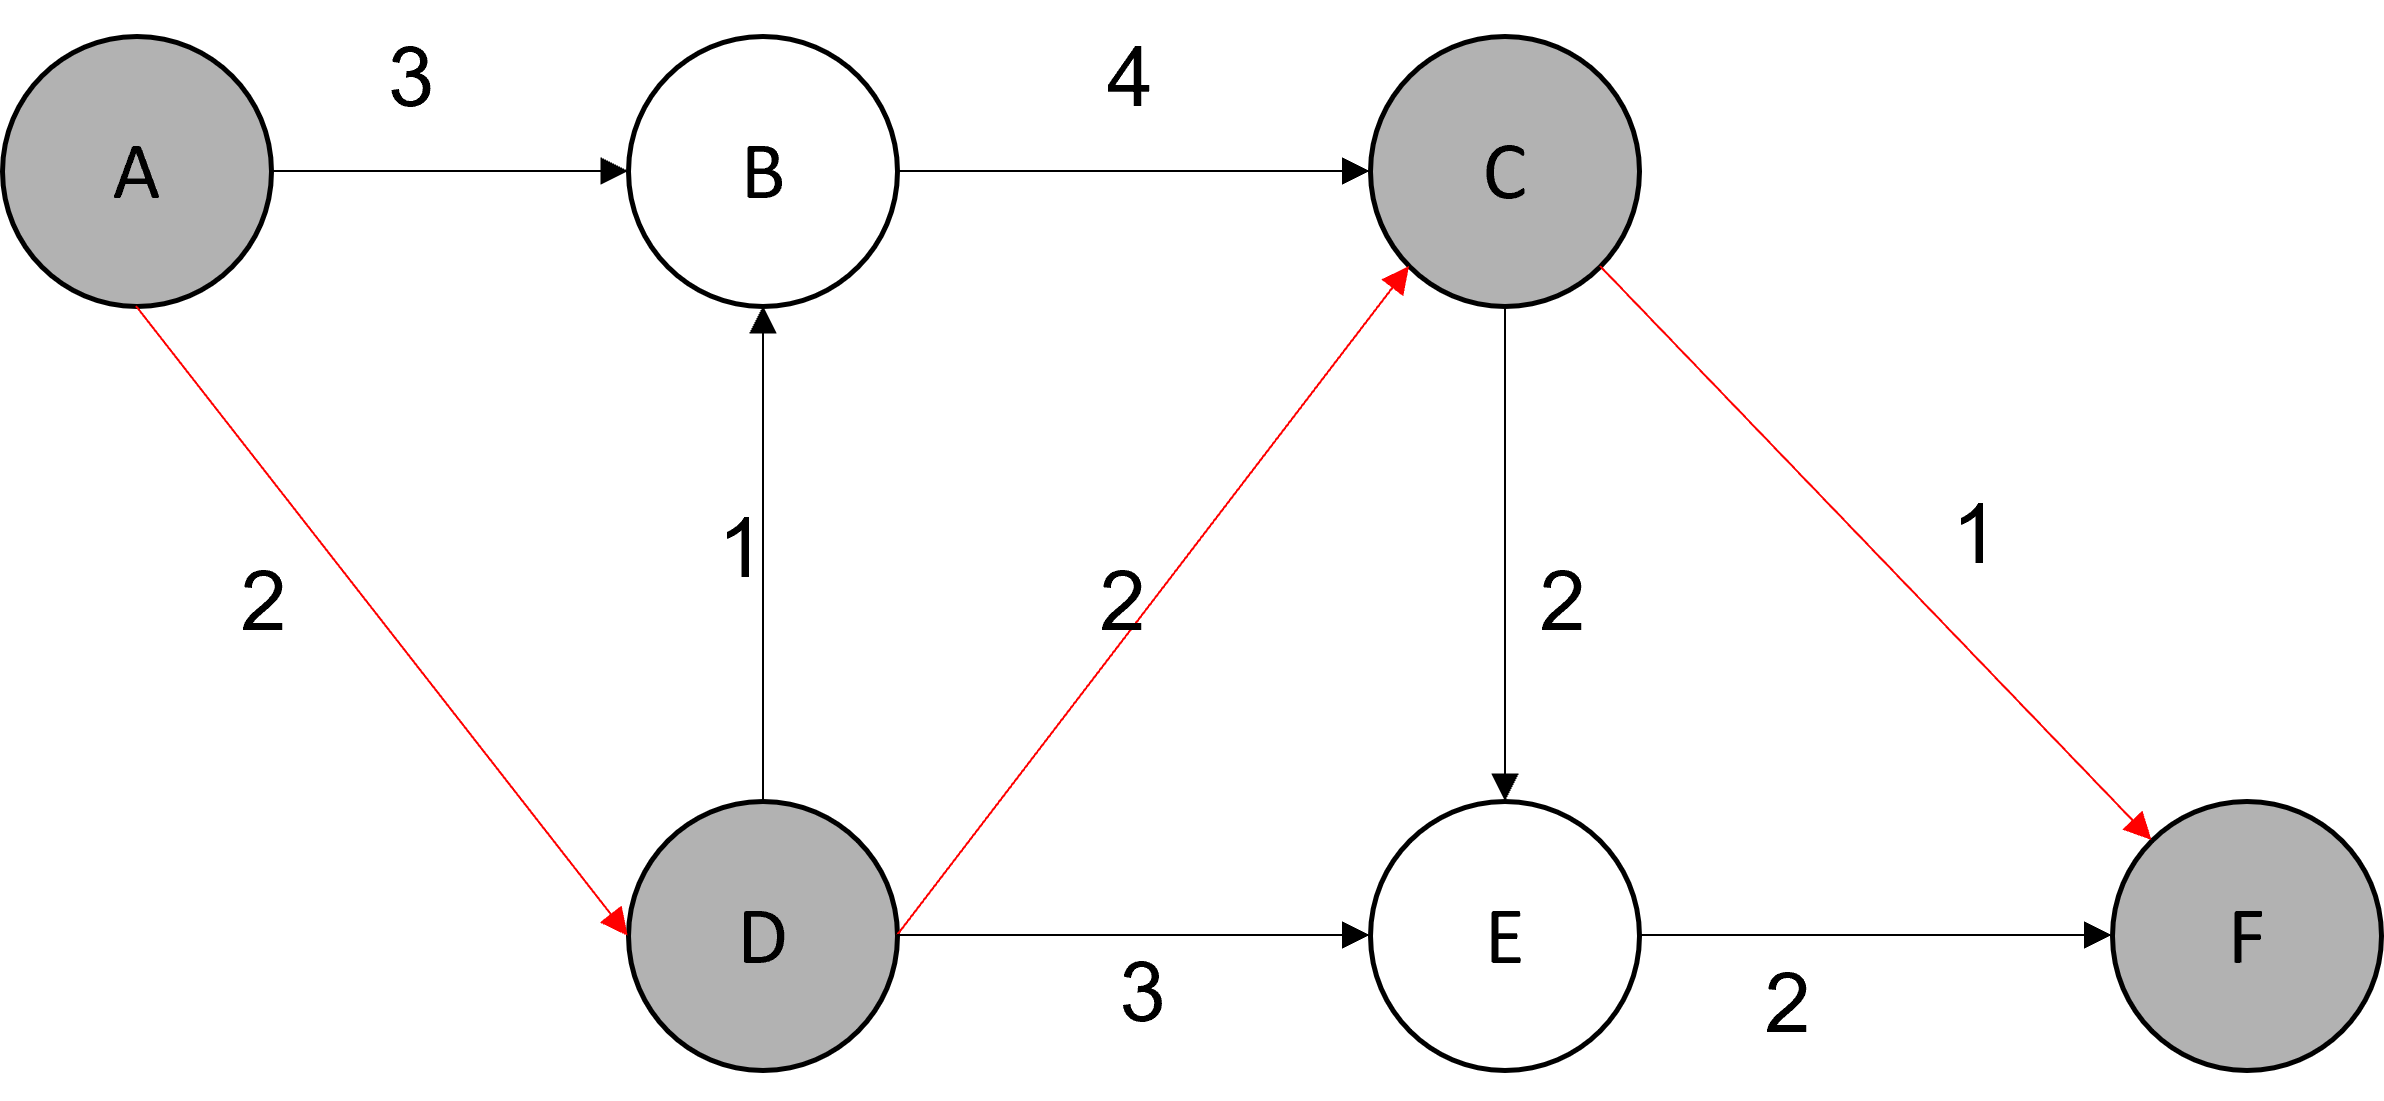
\includegraphics[width=0.6\textwidth]{png/图片18 最短路径A1} %插入图片,[]中设置图片大小,{}中是图片文件名
        \caption{最短路径$A^1$} %最终文档中希望显示的图片标题
        \label{fig:fig18} %用于文内引用的标签
    \end{figure}

    \item 将最短路径$A^1$中的所有路段添加到偏离点容器中,此时偏离点容器如图\ref{fig:fig19}所示
    \begin{figure}[H] %H为当前位置,!htb为忽略美学标准,htbp为浮动图形
        \centering %图片居中
        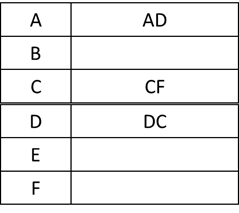
\includegraphics[width=0.45\textwidth]{png/图片18偏离点容器} %插入图片,[]中设置图片大小,{}中是图片文件名
        \caption{偏离点容器状态} %最终文档中希望显示的图片标题
        \label{fig:fig19} %用于文内引用的标签
    \end{figure}

    \item 依次以$A^1$中除汇点外的结点A,D,C作为偏离点,计算偏离路径,并添加到k最短路径的候选容器中,分别如图\ref{fig:fig20}
    \begin{figure}[htbp]
        \centering  %图片全局居中
        \subfigure[偏离路径$A_1^2$]{
            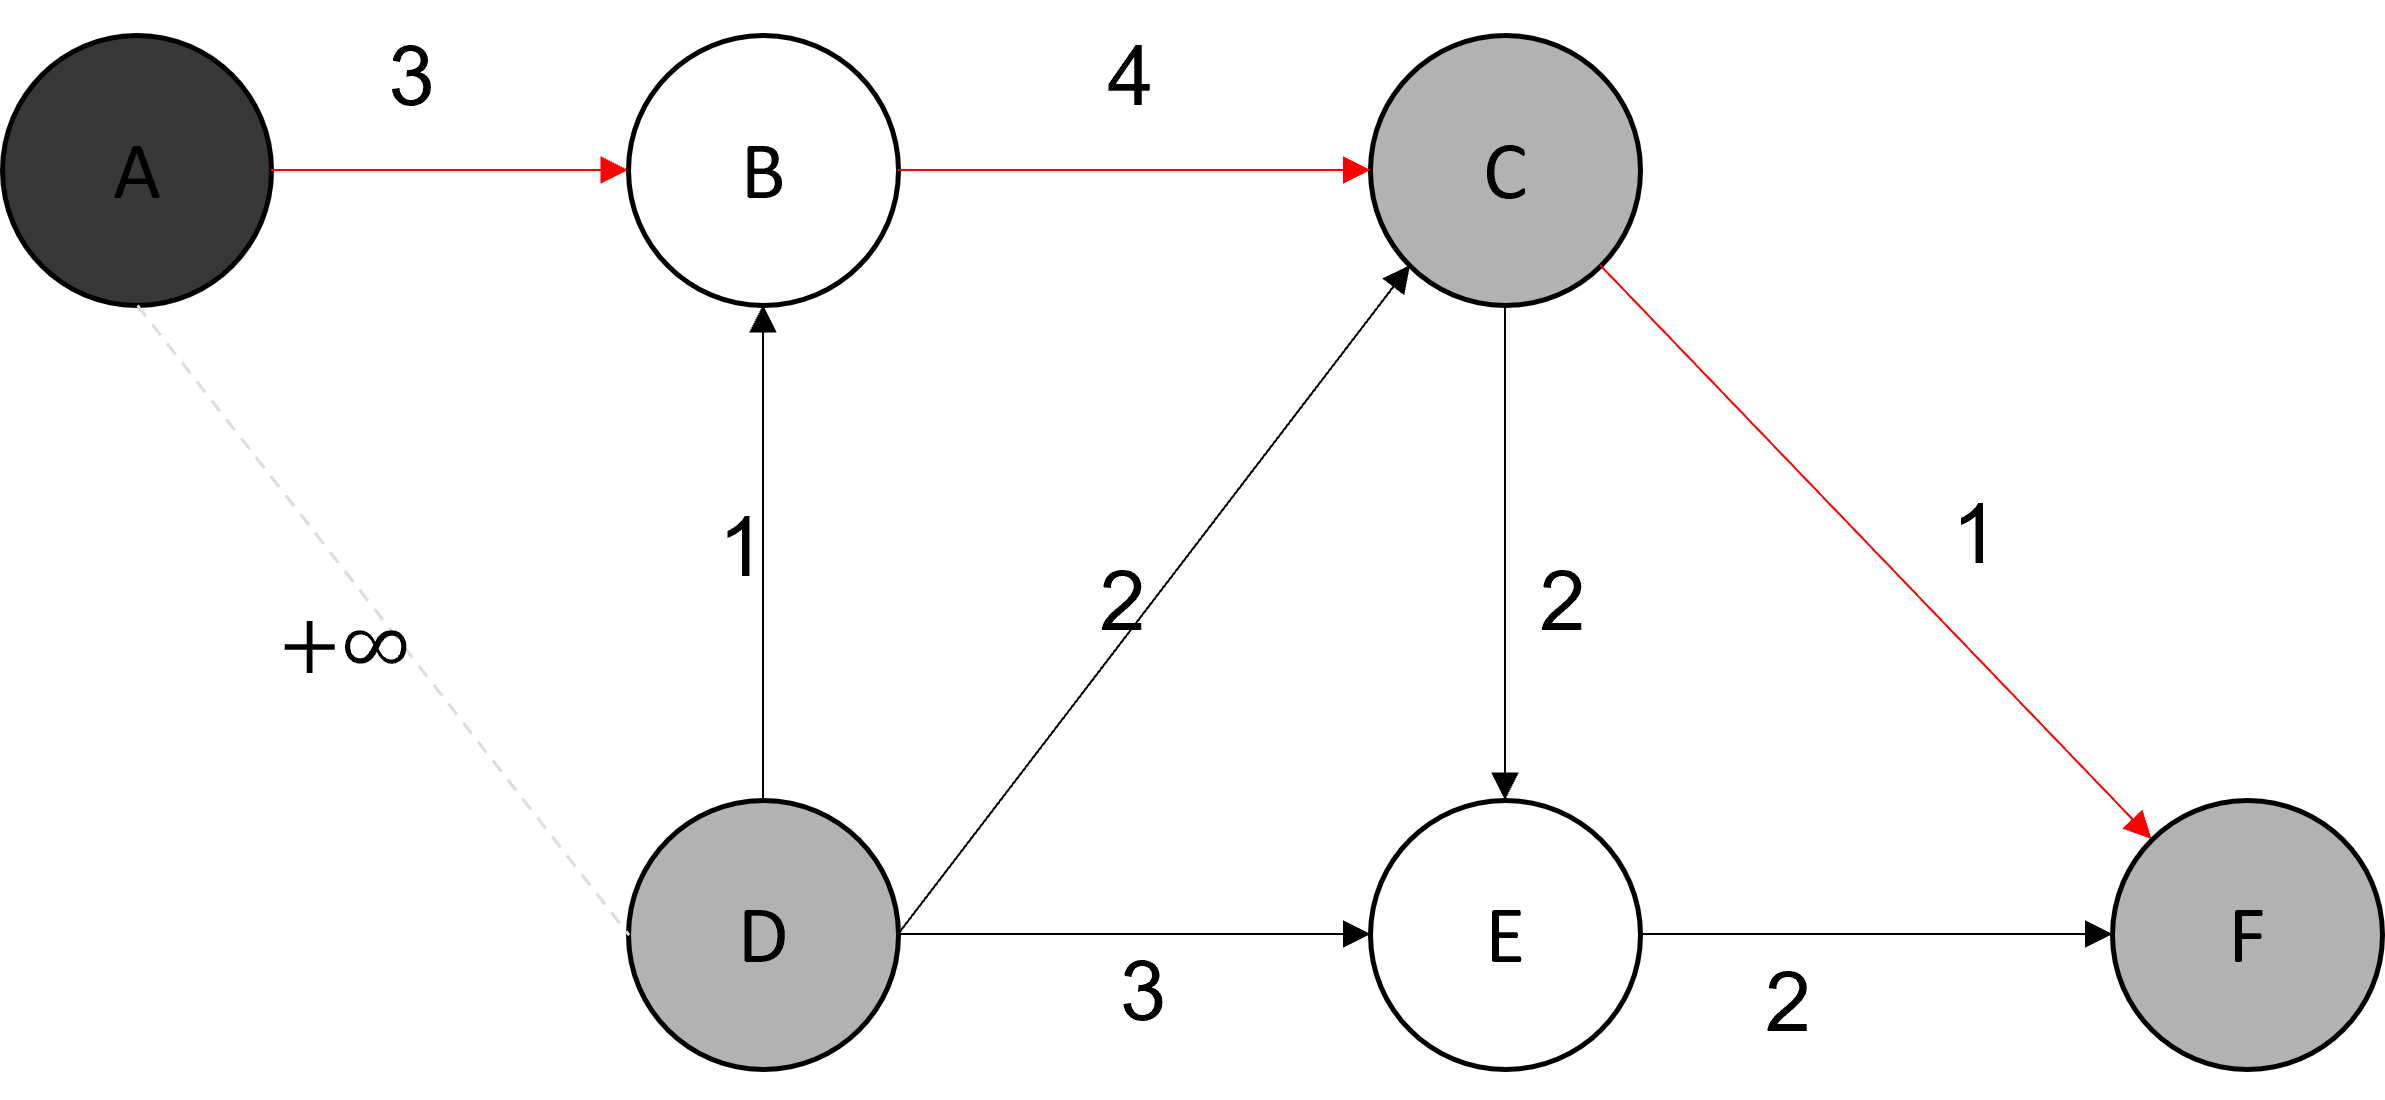
\includegraphics[width=0.45\textwidth]{png/图片19偏离路径A2_1的计算}}
        \quad
        \subfigure[偏离路径$A_2^2$]{
            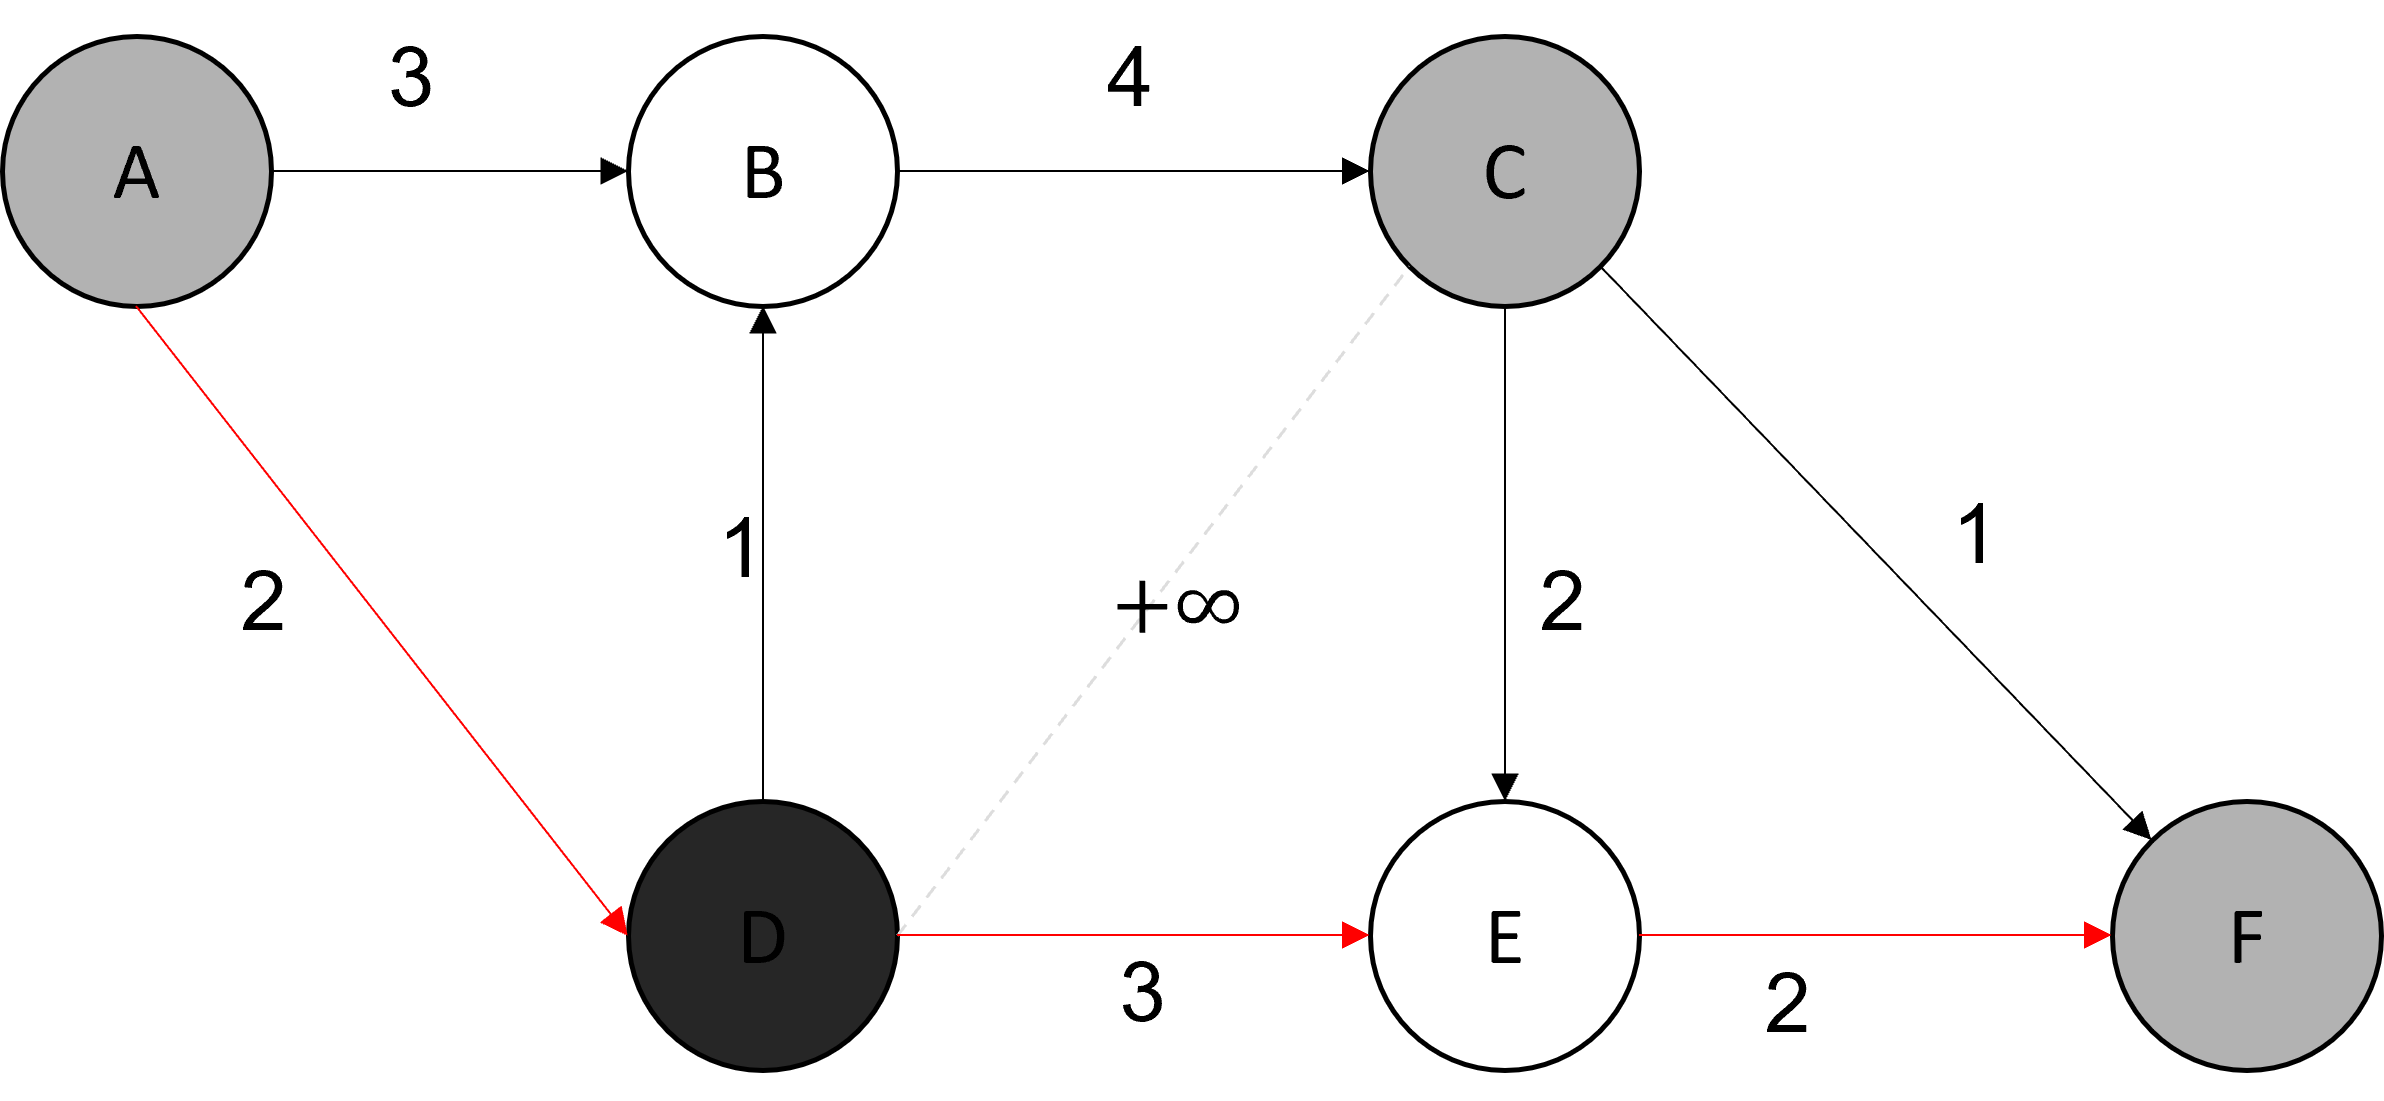
\includegraphics[width=0.45\textwidth]{png/图片20偏离路径A2_2的计算}}
        \quad
        \subfigure[偏离路径$A_3^2$]{
            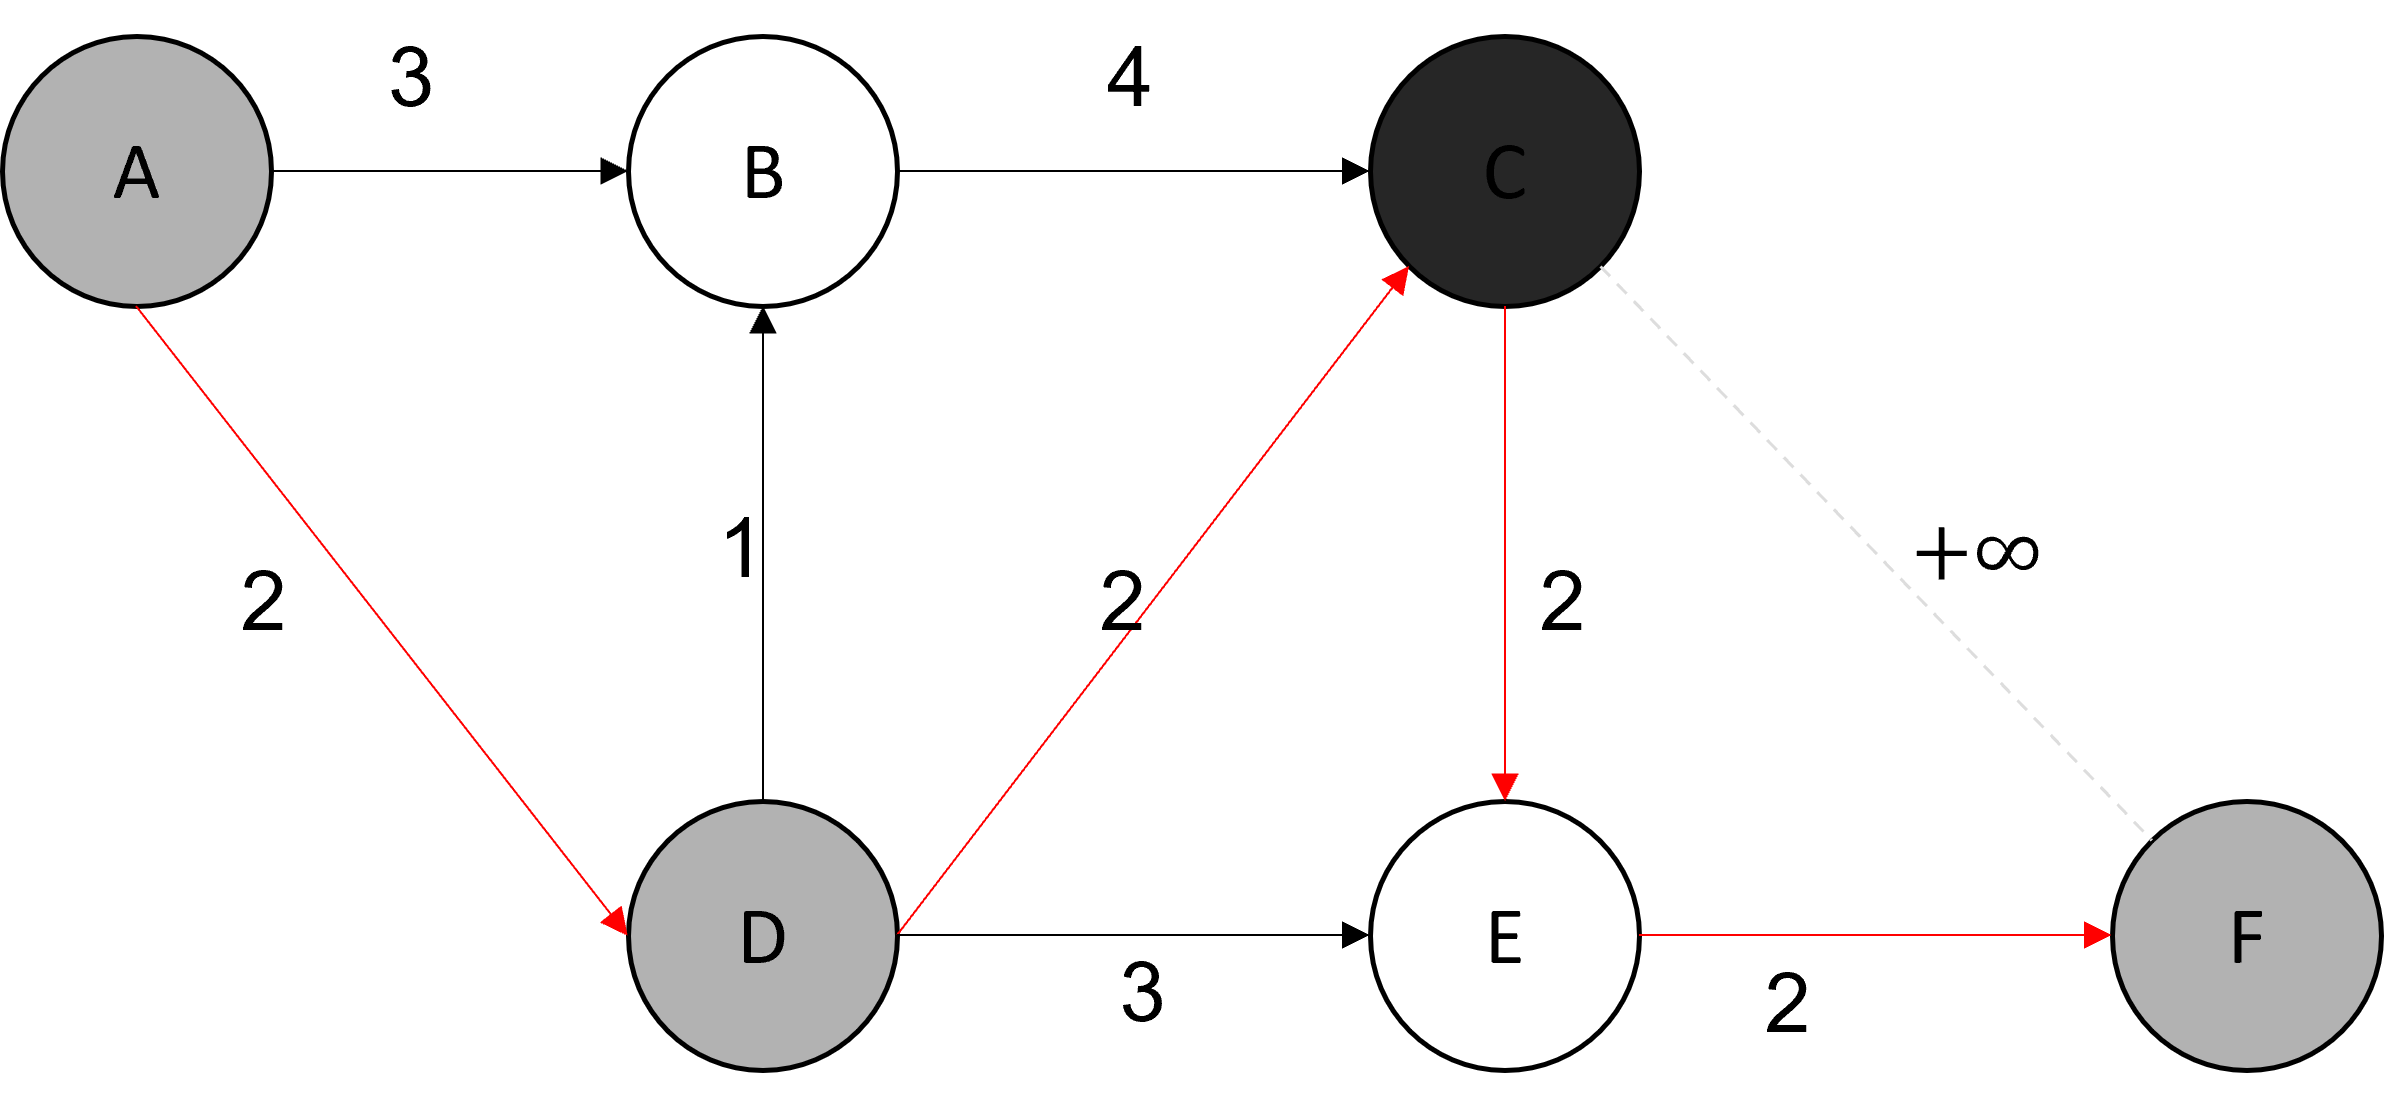
\includegraphics[width=0.45\textwidth]{png/图片21偏离路径A2_3的计算}}
        \quad
        \subfigure[最短路径$A^1$]{
            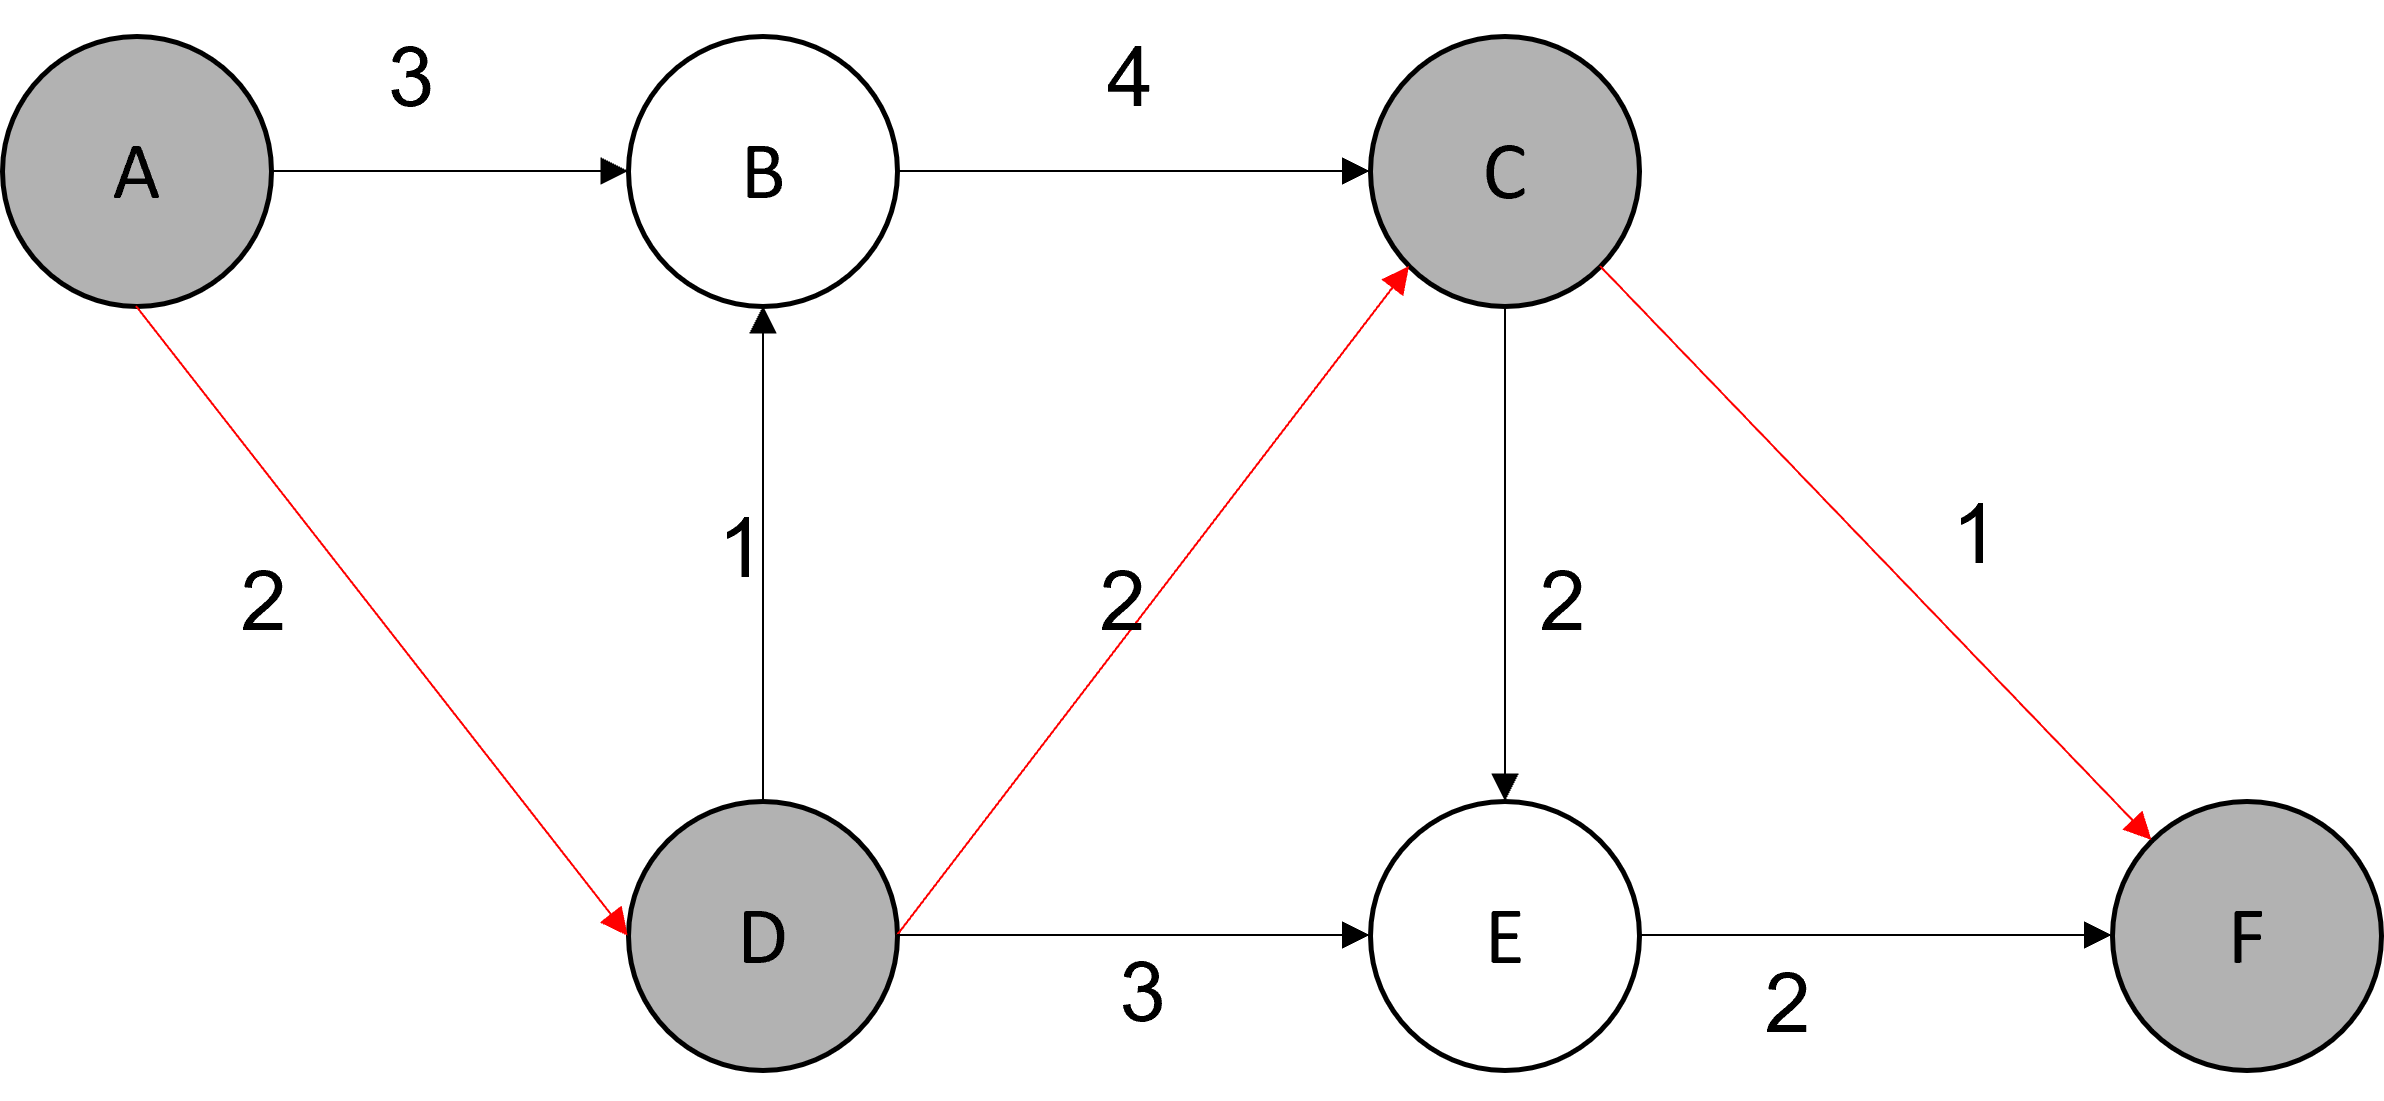
\includegraphics[width=0.45\textwidth]{png/图片18 最短路径A1}}
        \caption{偏离路径$A_i^2$的计算}
        \label{fig:fig20}
    \end{figure}

    \item 此时k最短路径候选容器状态如图\ref{fig:fig202}所示,从中选择最短的路径最为当前所求的k最短路径,显然此时最短路径为偏离路径$A_2^2$
    \begin{figure}[H] %H为当前位置,!htb为忽略美学标准,htbp为浮动图形
        \centering %图片居中
        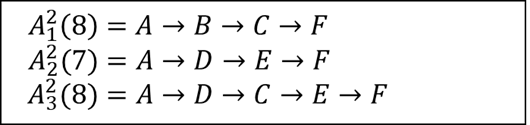
\includegraphics[width=0.7\textwidth]{png/图片20 k最短路径候选容器} %插入图片,[]中设置图片大小,{}中是图片文件名
        \caption{k最短路径候选容器} %最终文档中希望显示的图片标题
        \label{fig:fig202} %用于文内引用的标签
    \end{figure}

    \item 更新偏离点容器,容器状态如图\ref{fig:fig21}所示
    \begin{figure}[H] %H为当前位置,!htb为忽略美学标准,htbp为浮动图形
        \centering %图片居中
        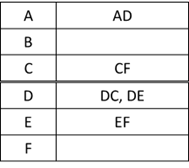
\includegraphics[width=0.45\textwidth]{png/图片21 更新偏离点容器} %插入图片,[]中设置图片大小,{}中是图片文件名
        \caption{更新偏离点容器} %最终文档中希望显示的图片标题
        \label{fig:fig21} %用于文内引用的标签
    \end{figure}

    \item 以A为偏离点,计算偏离路径$A_1^3$,如图\ref{fig:fig192}所示,发现此时$A_1^3=A\to B\to C \to F$已经出现在容器B中,因此不需要添加到容器之中;
    \begin{figure}[H] %H为当前位置,!htb为忽略美学标准,htbp为浮动图形
        \centering %图片居中
        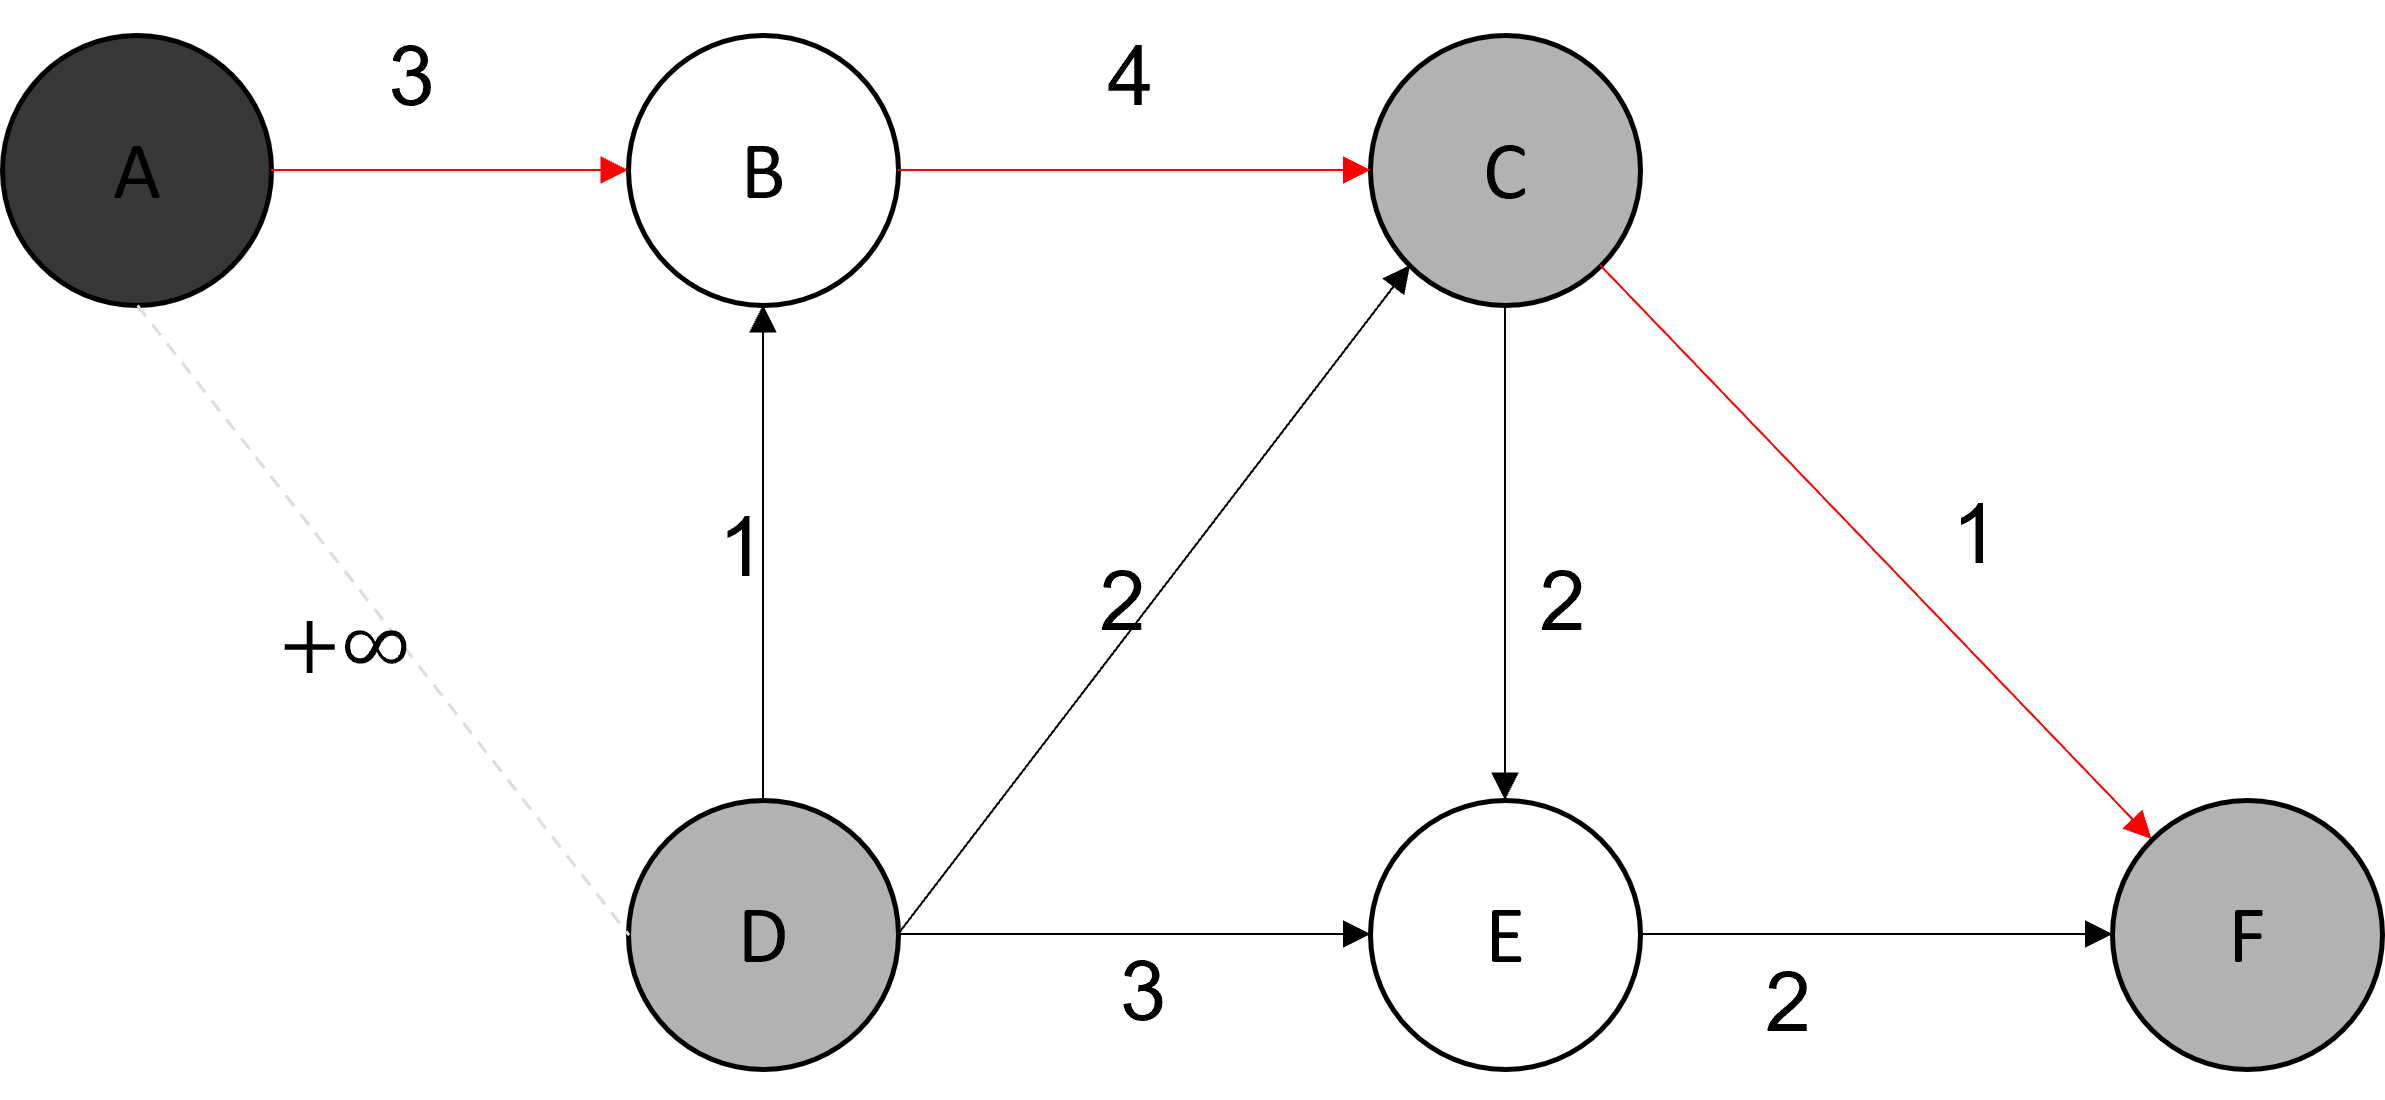
\includegraphics[width=0.7\textwidth]{png/图片19偏离路径A2_1的计算} %插入图片,[]中设置图片大小,{}中是图片文件名
        \caption{偏离路径$A_1^3$的计算} %最终文档中希望显示的图片标题
        \label{fig:fig192} %用于文内引用的标签
    \end{figure}

    \item 以D为偏离点,计算偏离路径$A_2^3(8)=A\to D\to B\to C\to F$,如图\ref{fig:fig27}所示,并添加到容器B中作为$A^3$的候选路径;
    \begin{figure}[H] %H为当前位置,!htb为忽略美学标准,htbp为浮动图形
        \centering %图片居中
        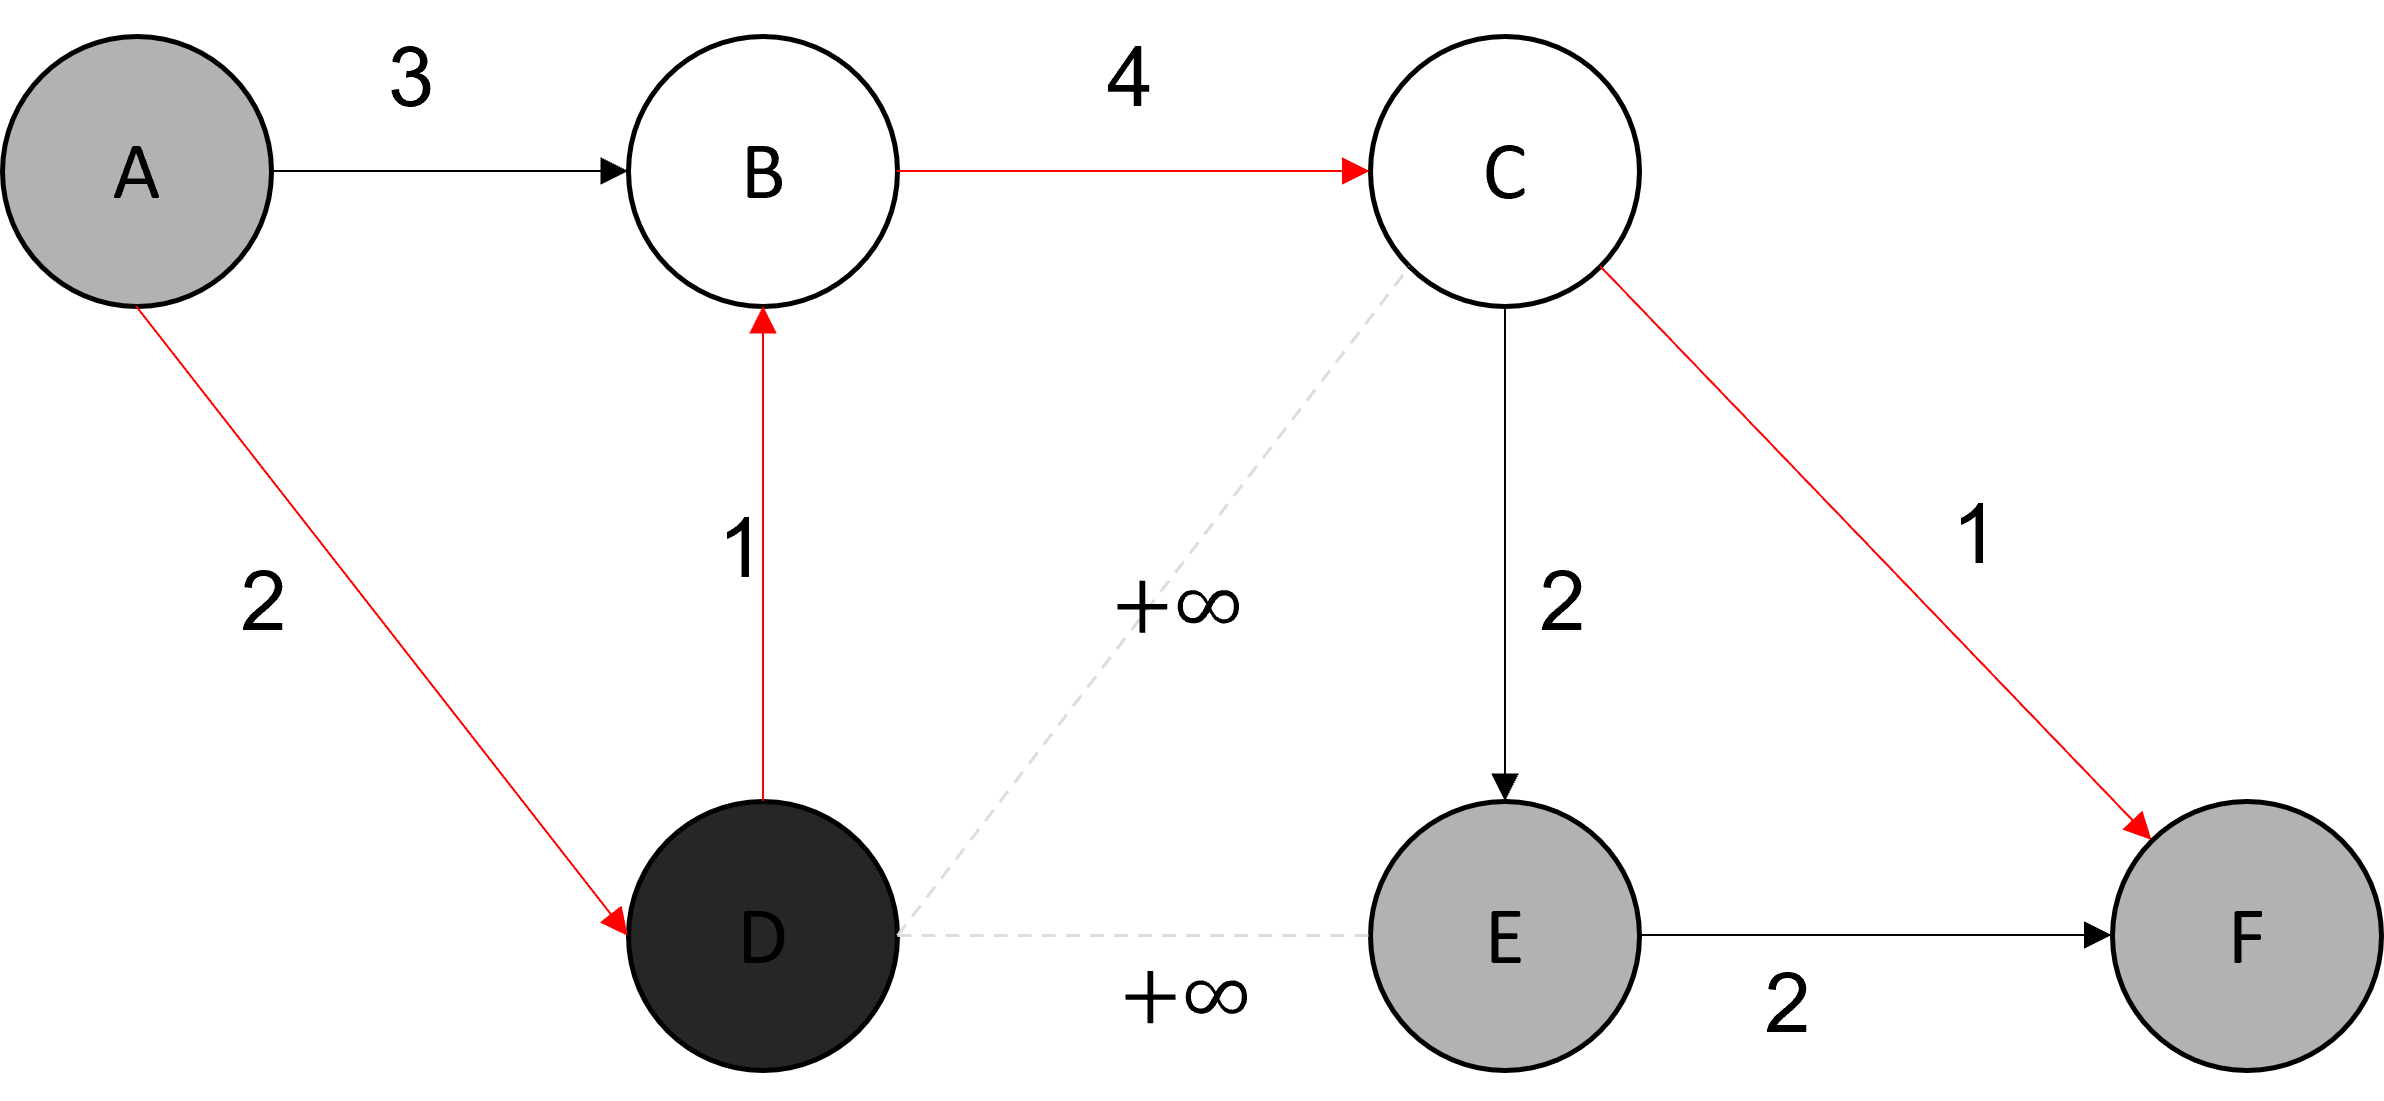
\includegraphics[width=0.7\textwidth]{png/图片27 偏离路径A3_2} %插入图片,[]中设置图片大小,{}中是图片文件名
        \caption{偏离路径$A^3_2$} %最终文档中希望显示的图片标题
        \label{fig:fig27} %用于文内引用的标签
    \end{figure}

    \item 以E为偏离点,计算偏离路径$A_3^3$,此时不存在以E为偏离点的偏离路径,如图\ref{fig:fig28}所示;
    \begin{figure}[H] %H为当前位置,!htb为忽略美学标准,htbp为浮动图形
        \centering %图片居中
        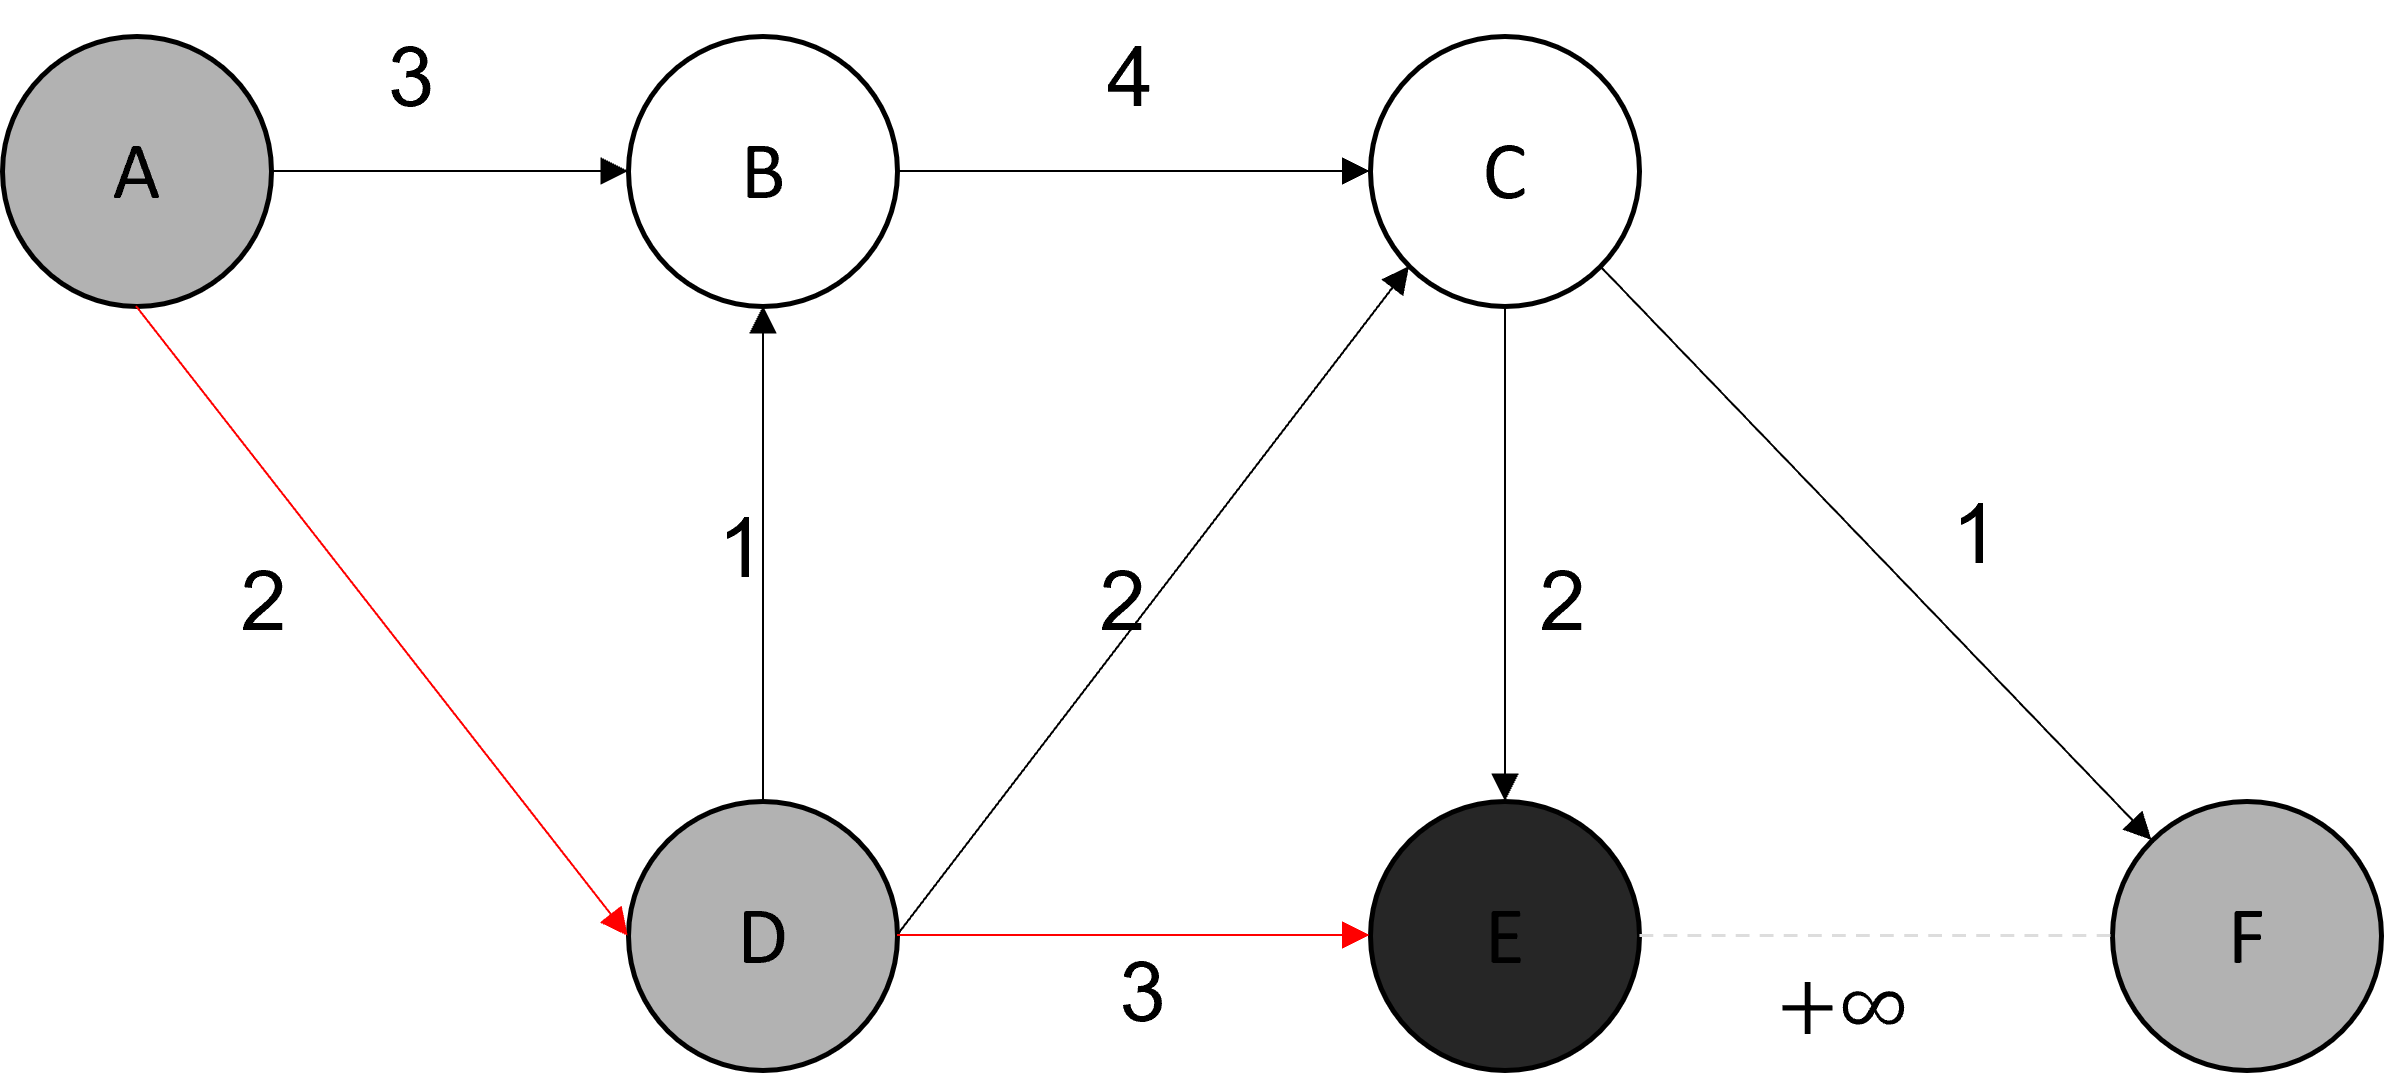
\includegraphics[width=0.7\textwidth]{png/图片28 不存在偏离路径A3_3} %插入图片,[]中设置图片大小,{}中是图片文件名
        \caption{不存在偏离路径$A^3_3$} %最终文档中希望显示的图片标题
        \label{fig:fig28} %用于文内引用的标签
    \end{figure}

    \item 从容器B取出最短路径,即$A^3=A\to D\to B\to C\to F$,自此算法执行完毕。
\end{enumerate}


\section{程序正确性验证}\label{sec:程序正确性验证}

\begin{figure}[H] %H为当前位置,!htb为忽略美学标准,htbp为浮动图形
    \centering %图片居中
    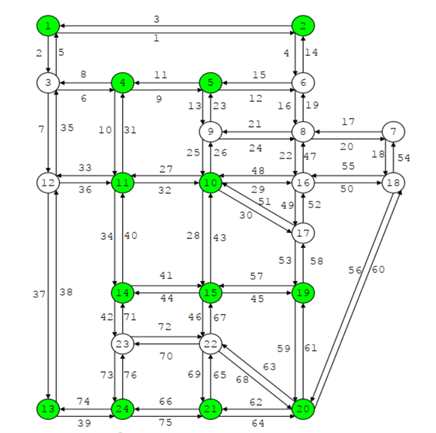
\includegraphics[width=0.7\textwidth]{png/图片22 SiouxFall测试网络} %插入图片,[]中设置图片大小,{}中是图片文件名
    \caption{SiouxFall测试网络} %最终文档中希望显示的图片标题
    \label{fig:fig22} %用于文内引用的标签
\end{figure}
分别对上述简单测试网络和如图\ref{fig:fig22}所示的Sioux Falls测试网络执行k最短路程序,对于SiouxFall测试网络输出前10条最短路如表\ref{tab:table1}所示,程序执行效果分别如图\ref{fig:fig23}, 图\ref{fig:fig24}所示。
程序运行结果和手工计算得到的结果完全相同,可以说明k最短路程序的正确性,因此下一章节将会将该程序用于规模更大、情况更加复杂的实际城市道路网络模拟中。
\begin{table}[H]
    \begin{center}
        \caption{SiouxFalls网络前10条无环最短路径及代价}\label{tab:table1}
        \begin{tabular}{ll}
            \hline
            最短路径                                                                                                                                                    & 路径成本 \\
            \hline
            $A^1= 1 \rightarrow 3 \rightarrow 12 \rightarrow 24$                                                                                                    & 85   \\
            $A^2= 1 \rightarrow 2 \rightarrow 6 \rightarrow 5 \rightarrow 4 \rightarrow 3 \rightarrow 12 \rightarrow 13 \rightarrow 24$     & 122  \\
            $A^3= 1 \rightarrow 3 \rightarrow 4 \rightarrow 11 \rightarrow 12 \rightarrow 13 \rightarrow 24$     & 127  \\
            $A^4= 1 \rightarrow 3 \rightarrow 4 \rightarrow 11 \rightarrow 14 \rightarrow 13 \rightarrow 24$     & 131  \\
            $A^5= 1 \rightarrow 2 \rightarrow 6 \rightarrow 5 \rightarrow 4 \rightarrow 11 \rightarrow 12 \rightarrow 13 \rightarrow 24$     & 150  \\
            $A^6= 1 \rightarrow 2 \rightarrow 6 \rightarrow 5 \rightarrow 4 \rightarrow 11 \rightarrow 14 \rightarrow 13 \rightarrow 24$     & 154  \\
            $A^7= 1 \rightarrow 3 \rightarrow 12 \rightarrow 11 \rightarrow 14 \rightarrow 13 \rightarrow 24$     & 158  \\
            $A^8= 1 \rightarrow 2 \rightarrow 6 \rightarrow 8 \rightarrow 9 \rightarrow 5 \rightarrow 4 \rightarrow 3 \rightarrow 12 \rightarrow 13 \rightarrow 23$     & 167  \\
            $A^9= 1 \rightarrow 3 \rightarrow 4 \rightarrow 11 \rightarrow 14 \rightarrow 23 \rightarrow 24$     & 167  \\
            $A^{10} = 1 \rightarrow 2 \rightarrow 6 \rightarrow 5 \rightarrow 4 \rightarrow 11 \rightarrow 14 \rightarrow 23 \rightarrow 24$ & 190  \\
            \hline
        \end{tabular}
    \end{center}
\end{table}

\begin{figure}[H] %H为当前位置,!htb为忽略美学标准,htbp为浮动图形
    \centering %图片居中
    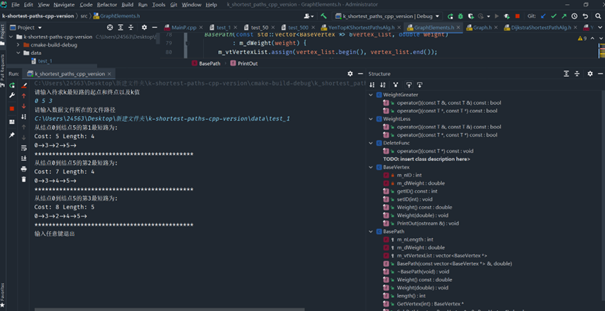
\includegraphics[width=0.9\textwidth]{png/图片23 6结点测试网络执行结果} %插入图片,[]中设置图片大小,{}中是图片文件名
    \caption{6结点测试网络执行结果} %最终文档中希望显示的图片标题
    \label{fig:fig23} %用于文内引用的标签
\end{figure}

\begin{figure}[H] %H为当前位置,!htb为忽略美学标准,htbp为浮动图形
    \centering %图片居中
    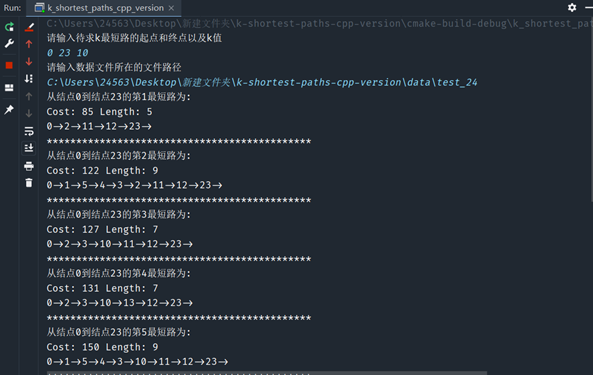
\includegraphics[width=0.9\textwidth]{png/图片24 SiouxFall测试网络执行结果} %插入图片,[]中设置图片大小,{}中是图片文件名
    \caption{SiouxFall测试网络执行结果} %最终文档中希望显示的图片标题
    \label{fig:fig24} %用于文内引用的标签
\end{figure}


\section{程序效率分析}\label{sec:程序效率分析}
在Sioux Falls测试网络程序可以很快的得到输出结果,之后对更大规模随机生成初始数据的网路进行程序的执行效率测试。
测试环境为Intel(R) Core(TM) i5-8300H CPU @ 2.30GHz和16GB的RAM,
测试在结点数和路段数分别在(a)24个结点50条路段、(b)50个结点1600条路段、(c)500个结点5800条路段、(d)800个结点8800条路段、(e)1000个结点11000条路段,
重复进行10次实验取平均值后统计程序执行时间,考虑到文件输入输出时间的不同,因此不包括文件的输入输出时间,程序执行时间结果如图\ref{fig:fig32}所示,可以发现程序执行时间大致随着边数呈现线性分布。
\begin{figure}[H] %H为当前位置,!htb为忽略美学标准,htbp为浮动图形
    \centering %图片居中
    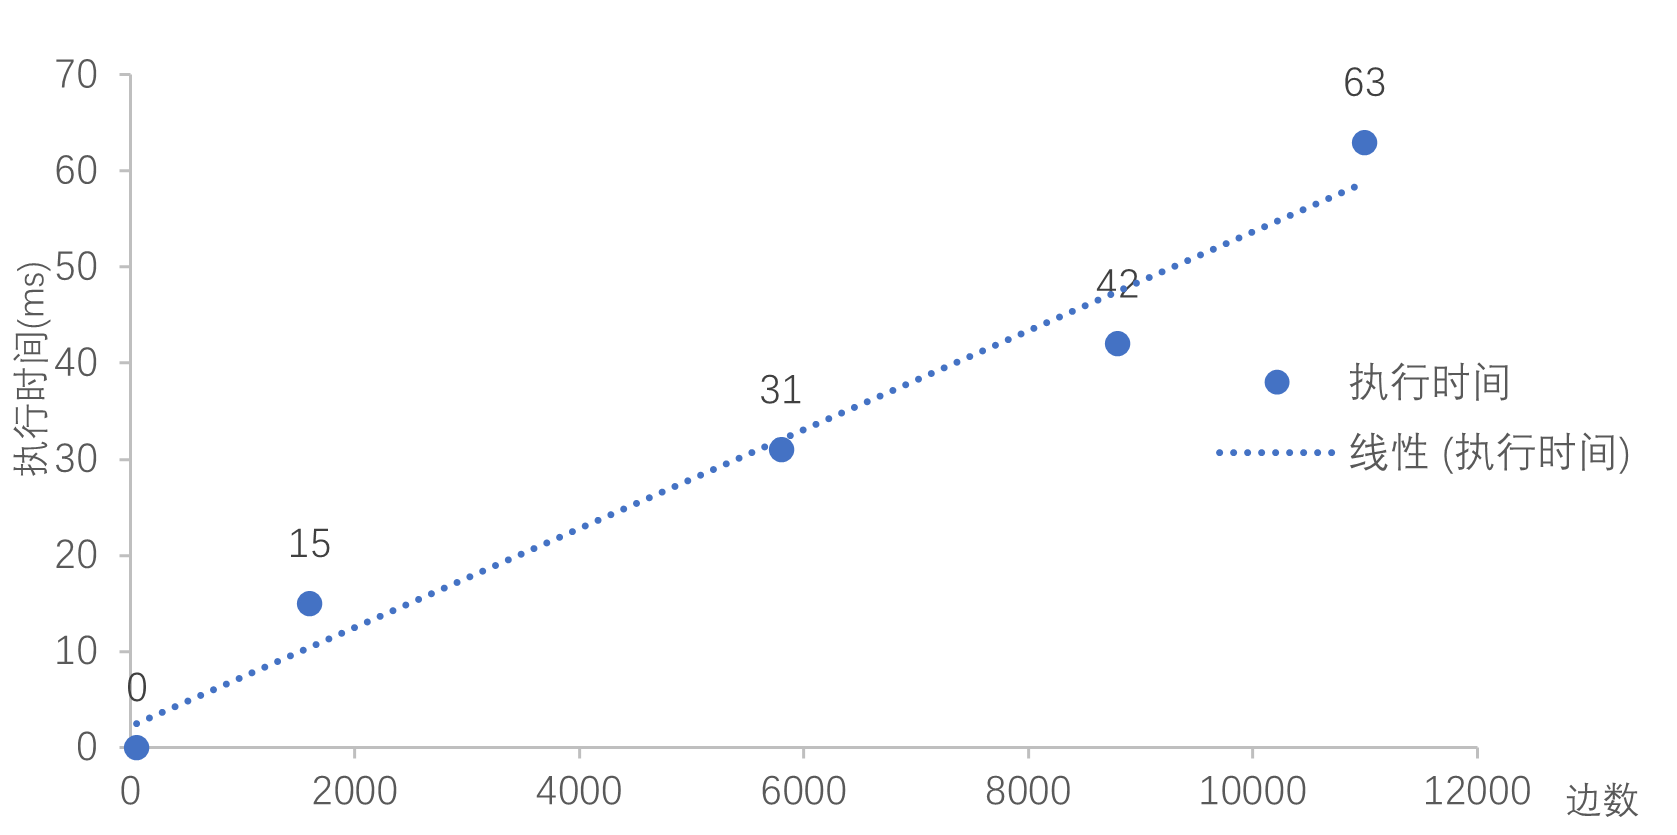
\includegraphics[width=0.7\textwidth]{png/图片32 程序执行时间与网络规模之间的关系} %插入图片,[]中设置图片大小,{}中是图片文件名
    \caption{程序执行时间与网络规模之间的关系} %最终文档中希望显示的图片标题
    \label{fig:fig32} %用于文内引用的标签
\end{figure}


\section{可靠性分析}\label{sec:可靠性分析}
可靠性是指在规定的条件下和规定的时间内,完成规定功能的能力。
在实际出行需求中,除考虑到出行者的距离花费和时间花费外,在特殊的场景中,往往还存在着可靠性要求。以常见的高铁出行方式中,出行者往往需要在特定的时间前到达高铁站,此时可能并不关注具体花费多长时间,而是需要赶在高铁出发前到达,类似这种应用场景下,路径可靠性要求将起到决定性的作用。
对道路系统而言,可靠度越高就越好。可靠度高的道路系统,可以长时间正常工作(这正是所有出行者需要得到的)。此外,高可靠性的道路系统还可以提供一定的道路故障容错,不会因为某条路段的道路维护造成行程时间的大幅度增加并对预计行程计划造成严重影响。

可靠度一般可分成两个层次,首先是所谓组件可靠度(Reliability of component)。也就是将产品拆解成若干不同的零件或组件,先就这些组件的可靠度进行研究,然后再探讨整个系统、整个产品的整体可靠度,也就是系统可靠度(Reliability of system)。
可靠度的概念不仅仅局限在交通系统中,但在交通系统中,可靠度可进一步划分。例如,组件可靠度可以进一步细分为连通可靠度和旅行时间可靠度,而系统可靠度则对应路网容量可靠度。

\subsection{出行时间可靠性分析}\label{subsec:出行时间可靠性分析}
驾驶者出行前通常都会估计正常情况下的行程时间,一般会选择提早出发时间来给道路系统提供一定的容错时间,但是出行时间不可能无限制的提前,因此对道路系统的可靠性作出相应的要求,可靠度的提高是反映交通管理效果的重要方面。此外,在考虑出行时间的可靠性的同时需要结合路网实际饱和度,路网容量,出行阻抗等因素综合考虑。出行时间可靠性是交通网络的随机性,路网运行的实际状态和驾驶者的决策行为共同作用的结果。通过路径诱导系统发布多条路线的行程时间和可靠性信息,可以有效地影响驾驶者的决策行为。

\subsection{连通可靠度分析}\label{subsec:连通可靠度分析}
行程时间可靠度的影响因素可能有如下方面:车辆抛锚,交通事故,交通信号灯,公交停靠站,车辆合流分流,交通流中大型车的比例,公路铁路交叉口的等待时间等。出行者会在自己的出行预算中增加一个预算时间,达到最终平衡。

可靠度的分类:连通可靠度,旅行时间可靠度,路网容量可靠度
\begin{itemize}%无序列表
    \item \textbf{连通可靠度}\\
    关注于网络拓扑结构的连通情况,关注网络中od对之间是否至少存在一条可行路径连通。而路段连通与否有两种状态:连通和不连通,分别使用1和0进行表示。
    在路段被破坏或维护时,可以认为路段不连通,或者当路段的交通流量是否超过路段容量,超过则认为不连通,此外还有学者提出当路段的交通流量超过某个阈值时可认为路段处于不连通的状态,这个阈值可以是某个固定值,可以是道路的初始容量,也可以是某个小于1的系数和道路容量的乘积。

    \item \textbf{旅行时间可靠度}\\
    在给定的时间间隔和要求的服务水平下,从指定出发点到指定目的地之间能够达到的概率。 可以用路段阻抗函数在给定时间间隔下的时间宽度比上总的时间长度。旅行时间可靠度本质上反映了行程时间的动态性和不确定性。

    \item \textbf{容量可靠度}\\
    在给定服务水平下网络容量能够适应一定交通需求的概率。
    交通网络中路段容量是会受到各种诸如时间,气候因素,天气状况,突发事件等各种不确定因素的影响而不断变化。交通网络的参与对象是人,具有一定的能动性和主观情感,不像其它货物,交通网络中的拥挤回由于拥挤产生延误,交通网络中的容量会受到路段容量,交通需求水平,拥挤,驾驶者的路径决策等的影响。
\end{itemize}



    \chapter{城市交通道路网络模拟}\label{ch:城市交通道路网络模拟}
在本案例学习过程中,对城市交通道路网络的构建采用开源平台Python + OpenStreetMap + Uber Movement。由于使用开源平台,因此对城市网络的构建是免费的,例如使用Google Maps API也可以构建道路网络,但是需要付费使用。此外Valhalla库也是开源的,可以作为备选项,但是Valhalla的学习曲线比较陡峭,需要花费大量时间和精力学习。基于上面的优缺点分析,选择使用Python中的Osmnx环境进行道路的构建模拟。


\section{Osmnx环境介绍与搭建}\label{sec:环境搭建}
OSMNX是一个Python软件包,可以从OpenStreetMap和模型,项目,可视化和分析现实世界中的街道网络以及任何其他地理空间几何形状下载地理空间数据。
可以使用Python代码下载并建模可步行,可驱动或骑自行车的城市网络,然后轻松分析和可视化它们。
也可以轻松地下载并使用其他基础设施类型,设施/兴趣点,建筑足迹,高程数据,街头轴承/方向以及速度/旅行时间。

由于Osmnx依赖于Anaconda,所以首先需要安装Anaconda环境,
然后使用conda config –prepend channel conda-forge和conda create -n ox –strict –channel-priority osmnx命令来创建osmnx环境。
安装完成后使用osmnx --version来检测osmnx环境是否安装成功,当在控制台出现osmnx的版本号时便表示环境搭建成功。

本文进行路网模拟测试实验所使用的环境为Python3.10 + Anaconda + OSMnx 1.1.2环境。


\section{数据准备}\label{sec:数据准备}
实验数据采用OpenStreetMap上获取的美国纽约市皇后区的街道道路信息和Uber Movement提供的相关的路段通行速度,部分数据信息见表\ref{tab:table}。
\begin{table}[H]
    \begin{center}
        \caption{纽约市皇后区城市道路信息(部分)}\label{tab:table}
        \begin{tabular}{llll}
            \hline
            id & osmWayId & hour & speed  \\
            \hline
            0  & 5029221  & 0    & 23.508 \\
            1  & 5029221  & 1    & 24.487 \\
            2  & 5029221  & 2    & 24.330 \\
            3  & 5029221  & 3    & 28.003 \\
            4  & 5029221  & 4    & 24.547 \\
            5  & 5029221  & 5    & 22.321 \\
            6  & 5029221  & 6    & 12.853 \\
            7  & 5029221  & 7    & 10.183 \\
            8  & 5029221  & 8    & 9.0898 \\
            9  & 5029221  & 9    & 11.414 \\
            10 & 5029221  & 10   & 12.677 \\
            11 & 5029221  & 11   & 12.395 \\
            12 & 5029221  & 12   & 13.598 \\
            13 & 5029221  & 13   & 13.382 \\
            14 & 5029221  & 14   & 13.656 \\
            15 & 5029221  & 15   & 11.505 \\
            \hline
        \end{tabular}
    \end{center}
\end{table}


\section{实验流程}\label{sec:实验流程}

\subsection{数据处理}\label{subsec:数据处理}
第一步需要根据街道道路信息创建道路网络,而OsMnx不仅可以对城市道路网络进行空间分析,同时也包含一系列用于创建道路网络和网络分析的函数。
其中包含由南加大规划系的Geoff Boeing教授编写的OpenStreetMap的python拓展增强包,
可以方便的进行城市道路网络的建模和对道路网络数据进行数据筛选,数据过滤,数据处理和数据分析。
借助这些工具包,配合OpenStreeMap可以很方便的构建出城市道路网络,并在其上进行城市道路网络状态的分析。

通过下面的代码首先可以创建出纽约市皇后区的城市道路网络,并对皇后区的城市道路网络数据
进行一个初步的过滤,程序中依据可达性分析的思想,避免边缘数据点对总体分布造成的极端影响,将连通节点数小于总节点数十分之一的部分节点看作为偏僻节点,其出行数据不作为最终结果的一部分。

\begin{lstlisting}[
    language=Python,
    morekeywords={as},
    label={lst:lstlisting5}
]
# 导入osmnx程序包
import osmnx as ox
# 构建纽约市皇后区城市道路网络图
G = ox.graph_from_place('Queens, New York, USA', network_type='drive')
# 准备一个列表, 用于存放待删除的边缘节点
remove_list = []
# 计算图中总的节点数量
num_nodes = len(G.nodes)
# 遍历图中的每一个节点, 计算其连通节点数量, 判断其是否为边缘节点
for node in G.nodes:
    # 计算当前节点的可达节点数
    reach = len(nx.descendants(G, node))
    # 判断可达节点数是否小于总节点数的1/10
    if reach < num_nodes / 10:
        # 如果是边缘节点, 则添加到列表中准备删除
        remove_list.append(node)
        # 删除所有的待删除节点
        for node in remove_list:
            G.remove_node(node)
            G = nx.convert_node_labels_to_integers(G, label_attribute='old_node_ID')
# 绘制出删除边缘节点后的城市道路网络图
ox.plot_graph(G)
\end{lstlisting}

\subsection{创建路网}\label{subsec:创建路网}
通过上面的数据处理,可以将获取到的每条街道的信息构建成一个交通网络,
其中包含表示每条街道交叉口的结点和表示每条街道各个方向的边。
同时由于该区域中网络结点数量多达19993个,街道数量更是达到542933条,
因此为了加快算法的收敛速度,选择将部分可达性较差的结点从网络中删除,
选择依据条件为:包含该结点的连通图中所含结点的数量小于总结点数量1/10的结点将会被从观察对象中剔除。
创建的纽约皇后区的路网对象如图\ref{fig:fig26}所示。

\begin{figure}[H] %H为当前位置,!htb为忽略美学标准,htbp为浮动图形
    \centering %图片居中
    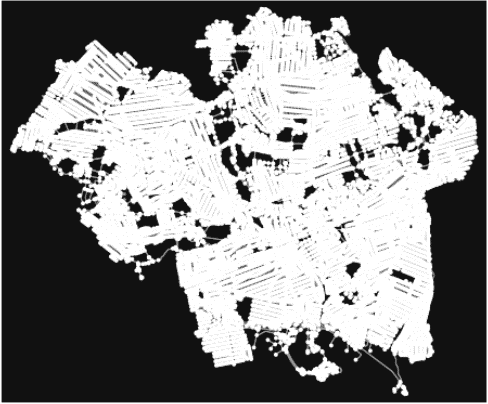
\includegraphics[width=0.7\textwidth]{png/图片26 纽约皇后区城市道路网} %插入图片,[]中设置图片大小,{}中是图片文件名
    \caption{纽约皇后区城市道路网} %最终文档中希望显示的图片标题
    \label{fig:fig26} %用于文内引用的标签
\end{figure}

\subsection{为路网附加时变行程时间}\label{subsec:为路网附加时变行程时间}
\begin{lstlisting}[
    language=Python,
    morekeywords={as},
    label={lst:lstlisting6}]
import osmnx as ox
import pandas as pd
# 为上面创建的纽约市皇后区的城市道路网络添加边属性
G = ox.add_edge_speeds(G)
# 为图中的边属性进行赋值, 保留小数点后一位
G = ox.speed.add_edge_travel_times(G, precision=1)
# 从OpenStreeMap下载的文件中读取道路网络中每一条边的最大行程速度
speed_df = pd.read_csv('nyc_avg_speeds_2019-06.csv')
# 根据距离和速度, 计算得到行程时间
speed_df = speed_df[['osm_way_id', 'hour', 'speed']]
speed_df.to_csv()
speed_dict = dict([((t.osm_way_id, t.hour), t.speed)
for t in speed_df.itertuples()])
speed_dict[(5029221, 12)]
\end{lstlisting}

为防止Uber提供的数据中没有直接给出路网的路段行程时间,
因此接下来通过已知的自由流的行程时间作为备用方案。
然后导入 Uber Movement 数据并转换为以 OSM Way ID 和一天中的小时为键的字典,
从而实现OpenStreetMap构建的路网的路段ID相匹配,并以一天为周期,
分别计算工作日内每个小时内的平均速度的平均值,得到路段通行速度,部分数据见表\ref{tab:table2},由于全部数据占用空间大,完整数据请通过附录\ref{ch:路网模拟实验代码}中代码生成。

\begin{table}[H]
    \caption{节点最短行程时间结果表(部分)}\label{tab:table2}
    \begin{tabular}{lllllllllllllllllllll}
        \hline
        & 0     & 1     & 2     & 3     & 4     & 5     & 6     & 7     & 8     & 9     \\
        \hline
        0  & 0.0   & 6.78  & 7.62  & 19.27 & 17.21 & 17.55 & 19.54 & 18.16 & 18.29 & 17.54 \\
        1  & 7.37  & 0.0   & 4.38  & 18.0  & 16.86 & 17.2  & 18.28 & 16.9  & 17.03 & 16.28 \\
        2  & 8.5   & 1.13  & 0.0   & 17.21 & 15.2  & 15.54 & 17.49 & 16.11 & 16.24 & 15.49 \\
        3  & 17.08 & 17.7  & 16.57 & 0.0   & 13.04 & 13.37 & 0.49  & 9.82  & 9.95  & 9.2   \\
        4  & 15.36 & 17.61 & 17.7  & 13.04 & 0.0   & 0.34  & 13.2  & 5.2   & 5.33  & 5.51  \\
        5  & 15.7  & 17.94 & 18.03 & 13.37 & 0.34  & 0.0   & 13.53 & 5.53  & 5.66  & 5.84  \\
        6  & 16.74 & 17.35 & 16.22 & 0.76  & 12.69 & 13.02 & 0.0   & 9.48  & 9.61  & 8.86  \\
        7  & 16.57 & 17.18 & 16.05 & 9.11  & 5.67  & 6.0   & 9.27  & 0.0   & 0.13  & 0.4   \\
        8  & 16.43 & 17.05 & 15.92 & 8.98  & 5.54  & 5.87  & 9.14  & 1.15  & 0.0   & 0.26  \\
        9  & 16.17 & 16.79 & 15.66 & 8.72  & 5.59  & 5.92  & 8.88  & 1.24  & 1.37  & 0.0   \\
        10 & 16.77 & 18.35 & 17.22 & 10.28 & 3.24  & 3.57  & 10.44 & 2.32  & 2.45  & 2.72  \\
        11 & 10.62 & 9.09  & 9.18  & 12.24 & 12.59 & 12.93 & 12.52 & 11.68 & 11.81 & 11.06 \\
        12 & 10.87 & 8.86  & 8.95  & 12.36 & 12.84 & 13.18 & 12.64 & 11.8  & 11.93 & 11.18 \\
        13 & 11.44 & 8.71  & 8.79  & 12.67 & 13.41 & 13.74 & 12.95 & 12.11 & 12.24 & 11.49 \\
        14 & 11.56 & 8.58  & 8.67  & 12.8  & 13.53 & 13.87 & 13.08 & 12.24 & 12.37 & 11.62 \\
        15 & 11.68 & 8.5   & 8.59  & 12.83 & 13.65 & 13.98 & 13.11 & 12.27 & 12.4  & 11.65 \\
        16 & 11.8  & 8.51  & 8.59  & 12.89 & 13.78 & 14.11 & 13.17 & 12.33 & 12.46 & 11.71 \\
        17 & 11.76 & 8.37  & 8.46  & 13.03 & 13.91 & 14.24 & 13.31 & 12.33 & 12.46 & 11.71 \\
        18 & 11.73 & 8.34  & 8.35  & 12.99 & 13.9  & 14.24 & 13.27 & 12.2  & 12.33 & 11.58 \\
        19 & 11.6  & 8.21  & 8.22  & 13.12 & 13.78 & 14.11 & 13.4  & 12.07 & 12.2  & 11.45 \\
        \hline
    \end{tabular}
\end{table}







    \chapter{结论与展望}\label{ch:结论与展望}


\section{论文主要结论}\label{sec:论文主要结论}
\begin{itemize}
    \item \textbf{多条最短路问题相较于最短路问题提供了更多的可选方案}\\
    虽然大多数出行者往往会选择距离最短的路径出行,但对于不同出行者实际的路径选择仍然存在差异,
    不同出行者可能选择距离最短,时间最短,保证在指定时间前到达,经过红绿灯最少,必须经过指定某地等不同的实际需求。
    最短路算法仅仅考虑了将出行者的需求局限在路径最短的条件之下,既不能满足其它需求用户的需要,也不利于改善服务提供商的提供的服务。
    此外当路网系统某一结点或路段发生故障时,最短路径可能恰好失效,需要重新计算最短路。对于大规模路网中计算所需的时间是不可忽略的,会造成极其糟糕的用户体验。
    多条最短路作为最短路问题的拓展,既满足了出行者差异化的需要, 又为路网系统提供了高可靠性和高容错性,还使得服务提供商能为用户提供更好的服务。

    \item \textbf{基于偏离路径思想实现的k最短路寻路程序满足在线实时路径推荐系统的需要}\\
    在给出的多条最短路求解案例中,通过偏离路径的思想对比了手工求解和程序求解,验证了算法设计和程序设计的正确性。
    偏离路径实现实现的k最短路算法不仅可以获得精确的k条最短路,同时能保证最短路径中不存在环路,符合交通领域的实际需要。
    并且在小于100000个结点的路网中,基于偏离路径实现k最短路寻路程序和基于启发式规则实现了A-star寻路程序的执行效率相差不大,仅仅在超大规模路网中A-star算法相较于偏离路径算法的速度更快。
    但A-star算法所计算出的最短路径中会出现环路,对于交通领域实际应用场景而言相当于在某个区域\lq\lq{绕圈}\rq\rq, 在一般交通场景应用而言,默认求解的是无环的最短路径,
    因此使用A-star算法计算的最短路需要额外考虑去除带环路径,此外A-star算法的运行效率和启发式规则的选择有关,并且所求的最短路径是实际最短路径的近似解。

    \item \textbf{时间空间网络中最短路问题不满足Bellman条件,不能使用双向搜索算法加速}\\
    时间空间网络和静态网络不同的地方之一在于路段阻抗随时间变化,因此对于实际交通流的描述能力更强,尤其是对于不同时间节点路段阻抗差异较大的网络。
    若A到C的最短路径为A $\to$ P1 $\to$ B $\to$ C,则静态网络中可以得到A到B的最短路径为A $\to$ P1 $\to$ B,
    不同于静态网络,时间空间网络的最短路不满足Bellman条件,最短路不仅取决于两个结点之间的路段阻抗还和上一个结点的状态有关,故A到B的最短路径可能为 A $\to$ P2 $\to$ B。
    双向搜索算法加速最短路径的寻找需要知道源点和汇点的节点状态,而时间空间网络中的最短路为动态最短路,即需要知道上一个节点的状态才能知道下一个结点的状态,因此不适用双向搜索算法的使用条件。

    \item \textbf{时间空间网络在满足周期性变化的条件下可以转化为静态网络来简化处理}\\
    交通网络不同于一般的静态网络,交通流在早晚高峰时段和平峰时段的路段阻抗存在较大差异,路段阻抗属于时变属性集,因此交通网络属于时变网络。
    此外交通网络有着自己独特的流量特点,呈现周期性的变化特点,且在微观上交通流的变化是连续的,而在宏观上交通流的变化是离散的,呈现出双峰分布的特点。
    因此时间空间网络中的多条最短路问题可以通过时间拓展图的处理方法转化为静态网络中多个源点序列到多个汇点序列的多条最短路问题。
\end{itemize}


\section{论文创新点}\label{sec:论文创新点}
本文的创新点分为两个部分:
\begin{enumerate}%有序列表
    \item \textbf{在模型构建层面,考虑了除路段外的节点阻抗,并通过拆点的方法将路段阻抗和节点阻抗实现形式上的统一}\\
    在时间空间网络模型的构建过程中,不仅考虑了路段阻抗,同时还考虑了结点阻抗,增强了时间空间网络模型对各种交通行为的表示能力,例如在交叉口转向,或者在地铁换乘站换乘等行为。
    同时基于拆点的思想,将结点拆分为N-S, N-W, N-E, S-N, S-W, S-E, W-S, W-N, W-E, E-S, E-N, E-W等12个方向的路段,并根据路段通行能力对结点阻抗进行分配。

    \item \textbf{在算法设计层面,实现了时间空间网络下的多条最短路算法设计和分别实现了有环最短路和无环最短路寻路程序}\\
    对时间空间网络中k最短路算法的求解拆分为三个主要流程: 第一是对时间空间网络进行离散化处理;
    第二是通过设计程序对时间空间网络进行时间拓展表示,从而达到将时间空间网络转化为一般物理网络,实现对问题的等价转化;
    第三是通过在静态网络中的k最短路设计来实现程序,从而实现最终问题的求解。
    设计的处理k最短路程序在优化之后很好地符合交通领域问题研究的实际特点: 最短路径中无环路,计算A地到C地的最短路径中会自动排除掉了A地 $\to$ B地 $\to$A地 $\to$C地这种不符合实际场景的路径推荐。

\end{enumerate}


\section{研究展望}\label{sec:研究展望}
在时间-空间网络中k条最短路算法的设计中,根据交通流的周期性和微观连续性以及宏观离散性的特点来对时间-空间网络中路段阻抗函数进行离散化处理是关键一步。离散化处理需要根据交通流量的实际情况进行进一步确定,在未来的研究中,可以基于时间空间序列分析方法,大数据和机器学习中来实现阻抗的离散化处理和阻抗的动态预测。

机器学习作为一种以数据驱动的建模范式,其模型的建立可以通过借助计算机从海量数据中练习获得,进一步的减少研究者主观因素选择导致的模型不确定性。机器学习模型需要大数据的支持,而对于路段中无时无刻不在生成的交通流量数据尤为合适,因此机器学习建模在大数据时代有着无与伦比的先天优势。

数据驱动下的交通科学正在蓬勃发展。即使获取到了大量数据,但关键是找到利用数据的方法,利用数据为出行者提供更好的服务。显然多条最短路问题的研究是符合这一趋势的,并且问题本身有较强的研究价值和进一步的拓展空间。

%\begin{figure}[H] %H为当前位置,!htb为忽略美学标准,htbp为浮动图形
%    \centering %图片居中
%    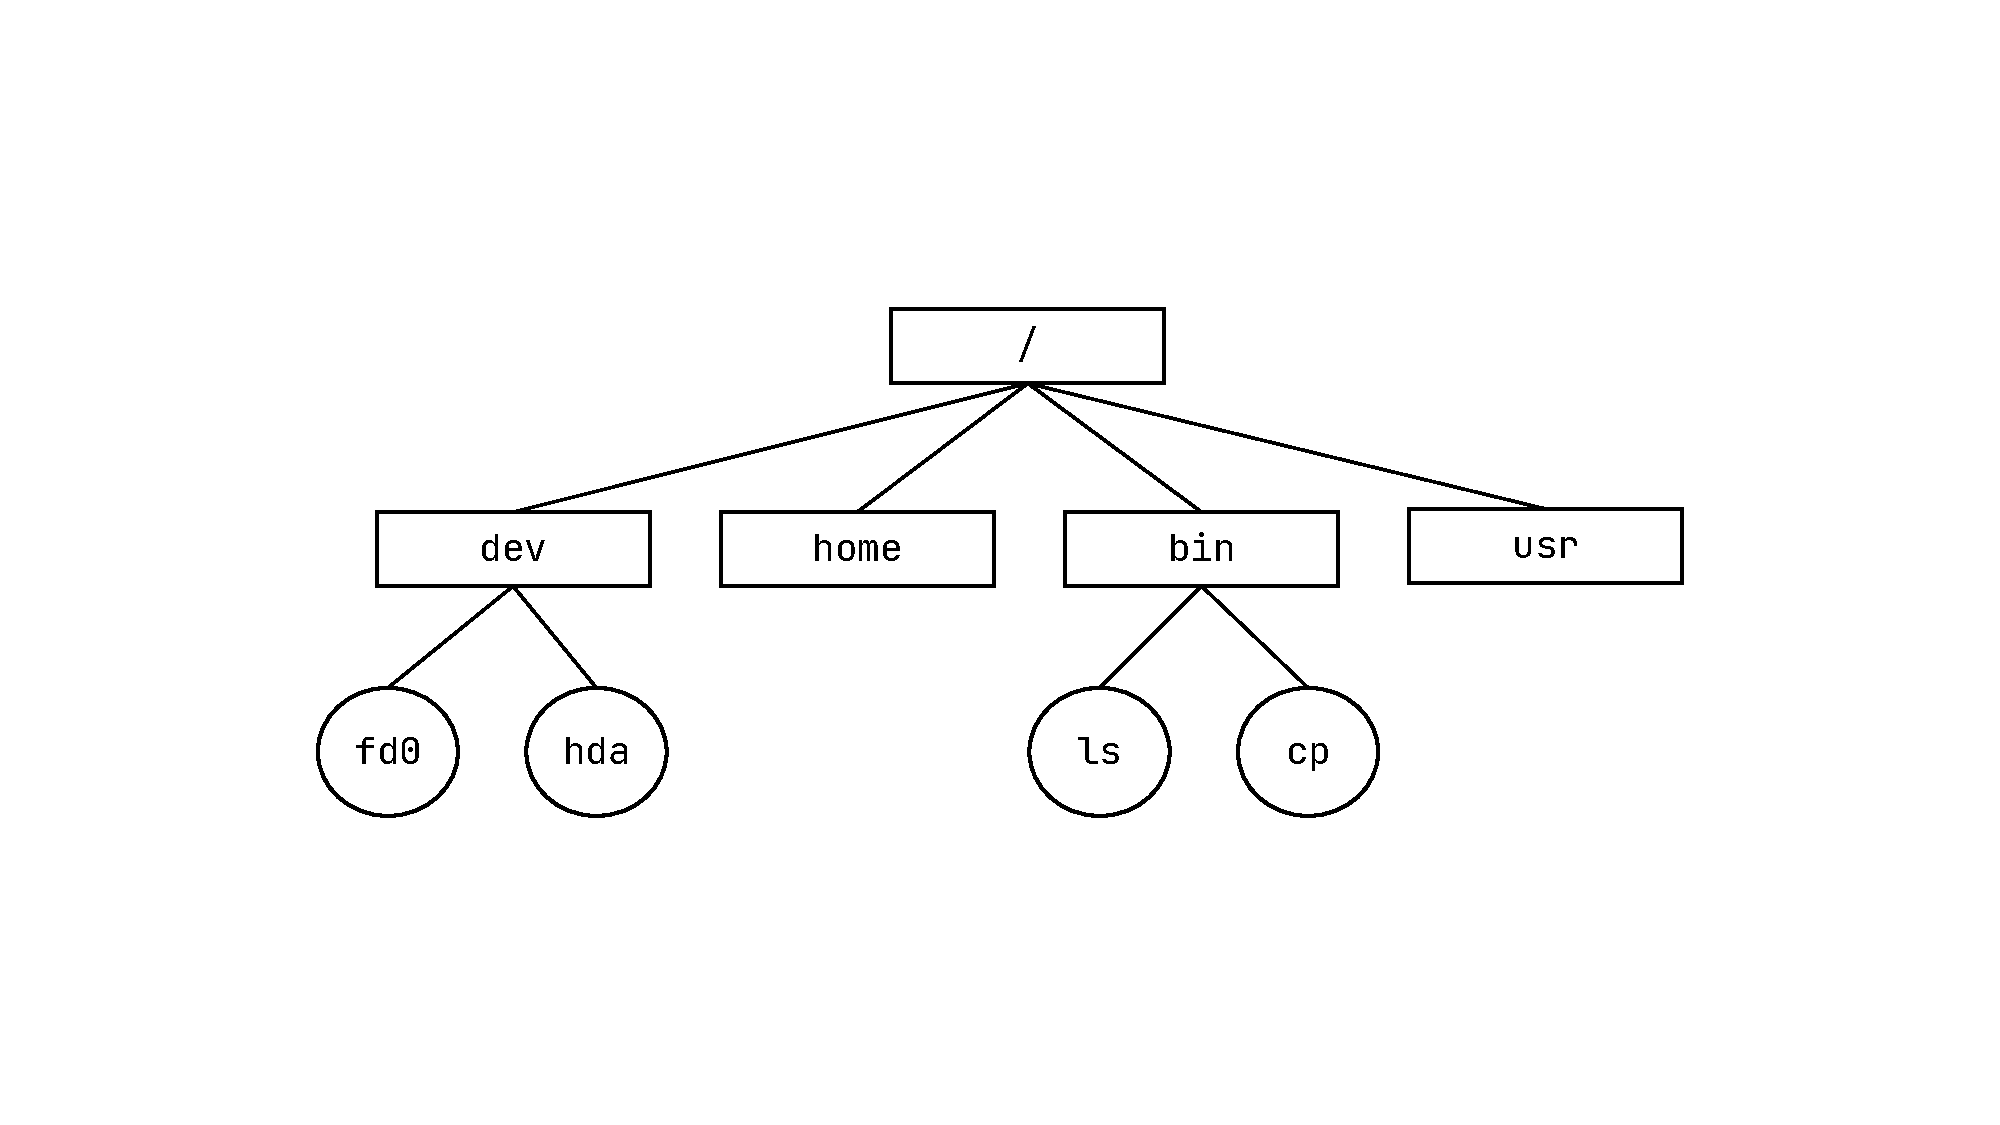
\includegraphics[width=0.7\textwidth]{png/book} %插入图片,[]中设置图片大小,{}中是图片文件名
%    \caption{book} %最终文档中希望显示的图片标题
%    \label{figx} %用于文内引用的标签
%\end{figure}
%如图\ref{figx}所示

%    参考文献
    \bibliographystyle{gbt7714-numerical}
    \bibliography{seuthesix}  % 告诉编译器参考文献所在文件
%    附录
    \appendix


\chapter{主程序}\label{ch:主程序}
\begin{lstlisting}[label={lst:lstlisting}]
#include <limits>
#include <set>
#include <map>
#include <queue>
#include <string>
#include <vector>
#include <fstream>
#include <iostream>
#include <algorithm>
#include "GraphElements.h"
#include "Graph.h"
#include "DijkstraShortestPathAlg.h"
#include "YenTopKShortestPathsAlg.h"
using namespace std;

void testDijkstraGraph() {
    Graph *my_graph_pt = new Graph("C:\\Users\\24563\\Desktop\\新建文件夹\\k-shortest-paths-cpp-version\\data\\test_15");
    DijkstraShortestPathAlg shortest_path_alg(my_graph_pt);
    BasePath *result = shortest_path_alg.get_shortest_path(my_graph_pt->get_vertex(0), my_graph_pt->get_vertex(14));
    result->PrintOut(cout);
}

void testYenAlg(int source, int sink, int k, string filename) {
    Graph my_graph(filename);

    YenTopKShortestPathsAlg yenAlg(my_graph, my_graph.get_vertex(source), my_graph.get_vertex(sink));


    int i = 0;
    while (yenAlg.has_next()) {
        ++i;
        cout << "从结点" << source << "到结点" << sink << "的第" << i << "最短路为:" << endl;
        yenAlg.next()->PrintOut(cout);
        if (i == k) {
            break;
        }
    }
}

int main(...) {
    cout << "请输入待求k最短路的起点和终点以及k值" << endl;
    int source;
    int sink;
    int k;
    cin >> source >> sink >> k;
    cout << "请输入数据文件所在的文件路径" << endl;
    string filepath = "C:\\Users\\24563\\Desktop\\新建文件夹\\k-shortest-paths-cpp-version\\data\\test_1";
    cin >> filepath;
    testYenAlg(source, sink, k, filepath);
    int flag;
    cout << "输入任意键退出" << endl;
    cin >> flag;
    return 0;
}


\end{lstlisting}


\chapter{K最短路实现}\label{ch:k最短路实现}
\begin{lstlisting}[
    language=C++,
    basicstyle=\ttfamily,
    breaklines=true,
    label={lst:lstlisting2}]
#include <set>
#include <map>
#include <queue>
#include <vector>
#include "GraphElements.h"
#include "Graph.h"
#include "DijkstraShortestPathAlg.h"
#include "YenTopKShortestPathsAlg.h"

using namespace std;

void YenTopKShortestPathsAlg::clear() {
    m_nGeneratedPathNum = 0;
    m_mpDerivationVertexIndex.clear();
    m_vResultList.clear();
    m_quPathCandidates.clear();
}

void YenTopKShortestPathsAlg::_init() {
    clear();
    if (m_pSourceVertex != NULL && m_pTargetVertex != NULL) {
        BasePath *pShortestPath = get_shortest_path(m_pSourceVertex, m_pTargetVertex);
        if (pShortestPath != NULL && pShortestPath->length() > 1) {
            m_quPathCandidates.insert(pShortestPath);
            m_mpDerivationVertexIndex[pShortestPath] = m_pSourceVertex;
        }
    }
}

BasePath *YenTopKShortestPathsAlg::get_shortest_path(BaseVertex *pSource, BaseVertex *pTarget) {
    DijkstraShortestPathAlg dijkstra_alg(m_pGraph);
    return dijkstra_alg.get_shortest_path(pSource, pTarget);
}

bool YenTopKShortestPathsAlg::has_next() {
    return !m_quPathCandidates.empty();
}

BasePath *YenTopKShortestPathsAlg::next() {
    //1. Prepare for removing vertices and arcs
    BasePath *cur_path = *(m_quPathCandidates.begin());//m_quPathCandidates.top();

    //m_quPathCandidates.pop();
    m_quPathCandidates.erase(m_quPathCandidates.begin());
    m_vResultList.push_back(cur_path);

    int count = m_vResultList.size();

    BaseVertex *cur_derivation_pt = m_mpDerivationVertexIndex.find(cur_path)->second;
    vector<BaseVertex *> sub_path_of_derivation_pt;
    cur_path->SubPath(sub_path_of_derivation_pt, cur_derivation_pt);
    int sub_path_length = sub_path_of_derivation_pt.size();

    //2. Remove the vertices and arcs in the graph
    for (int i = 0; i < count - 1; ++i) {
        BasePath *cur_result_path = m_vResultList.at(i);
        vector<BaseVertex *> cur_result_sub_path_of_derivation_pt;

        if (!cur_result_path->SubPath(cur_result_sub_path_of_derivation_pt, cur_derivation_pt)) continue;

        if (sub_path_length != cur_result_sub_path_of_derivation_pt.size()) continue;

        bool is_equal = true;
        for (int i = 0; i < sub_path_length; ++i) {
            if (sub_path_of_derivation_pt.at(i) != cur_result_sub_path_of_derivation_pt.at(i)) {
                is_equal = false;
                break;
            }
        }
        if (!is_equal) continue;

        //
        BaseVertex *cur_succ_vertex = cur_result_path->GetVertex(sub_path_length + 1);
        m_pGraph->remove_edge(make_pair(cur_derivation_pt->getID(), cur_succ_vertex->getID()));
    }

    //2.1 remove vertices and edges along the current result
    int path_length = cur_path->length();
    for (int i = 0; i < path_length - 1; ++i) {
        m_pGraph->remove_vertex(cur_path->GetVertex(i)->getID());
        m_pGraph->remove_edge(make_pair(cur_path->GetVertex(i)->getID(), cur_path->GetVertex(i + 1)->getID()));
    }

    //3. Calculate the shortest tree rooted at target vertex in the graph
    DijkstraShortestPathAlg reverse_tree(m_pGraph);
    reverse_tree.get_shortest_path_flower(m_pTargetVertex);

    //4. Recover the deleted vertices and update the cost and identify the new candidates results
    bool is_done = false;
    for (int i = path_length - 2; i >= 0 && !is_done; --i) {
        //4.1 Get the vertex to be recovered
        BaseVertex *cur_recover_vertex = cur_path->GetVertex(i);
        m_pGraph->recover_removed_vertex(cur_recover_vertex->getID());

        //4.2 Check if we should stop continuing in the next iteration
        if (cur_recover_vertex->getID() == cur_derivation_pt->getID()) {
            is_done = true;
        }

        //4.3 Calculate cost using forward star form
        BasePath *sub_path = reverse_tree.update_cost_forward(cur_recover_vertex);

        //4.4 Get one candidate result if possible
        if (sub_path != NULL) {
            ++m_nGeneratedPathNum;

            //4.4.1 Get the prefix from the concerned path
            double cost = 0;
            reverse_tree.correct_cost_backward(cur_recover_vertex);

            vector<BaseVertex *> pre_path_list;
            for (int j = 0; j < path_length; ++j) {
                BaseVertex *cur_vertex = cur_path->GetVertex(j);
                if (cur_vertex->getID() == cur_recover_vertex->getID()) {
                    //j = path_length;
                    break;
                } else {
                    cost += m_pGraph->get_original_edge_weight(cur_path->GetVertex(j), cur_path->GetVertex(1 + j));
                    pre_path_list.push_back(cur_vertex);
                }
            }
            //
            for (int j = 0; j < sub_path->length(); ++j) {
                pre_path_list.push_back(sub_path->GetVertex(j));
            }

            //4.4.2 Compose a candidate
            double weight_cost = cost + sub_path->Weight();
            delete sub_path;
            sub_path = new Path(pre_path_list, weight_cost);

            //4.4.3 Put it in the candidate pool if new
            if (m_mpDerivationVertexIndex.find(sub_path) == m_mpDerivationVertexIndex.end()) {
                m_quPathCandidates.insert(sub_path);
                m_mpDerivationVertexIndex[sub_path] = cur_recover_vertex;
            }
        }

        //4.5 Restore the edge
        BaseVertex *succ_vertex = cur_path->GetVertex(i + 1);
        m_pGraph->recover_removed_edge(make_pair(cur_recover_vertex->getID(), succ_vertex->getID()));

        //4.6 Update cost if necessary
        double cost_1 = m_pGraph->get_edge_weight(cur_recover_vertex, succ_vertex) + reverse_tree.get_start_distance_at(succ_vertex);

        if (reverse_tree.get_start_distance_at(cur_recover_vertex) > cost_1) {
            reverse_tree.set_start_distance_at(cur_recover_vertex, cost_1);
            reverse_tree.set_predecessor_vertex(cur_recover_vertex, succ_vertex);
            reverse_tree.correct_cost_backward(cur_recover_vertex);
        }
    }

    //5. Restore everything
    m_pGraph->recover_removed_edges();
    m_pGraph->recover_removed_vertices();

    return cur_path;
}

void YenTopKShortestPathsAlg::get_shortest_paths(BaseVertex *pSource, BaseVertex *pTarget, int top_k, vector<BasePath *> &result_list) {
    m_pSourceVertex = pSource;
    m_pTargetVertex = pTarget;

    _init();
    int count = 0;
    while (has_next() && count < top_k) {
        next();
        ++count;
    }

    result_list.assign(m_vResultList.begin(), m_vResultList.end());
}
\end{lstlisting}


\chapter{时间拓展图转化为静态网络}\label{ch:时间拓展图转化为静态网络}
\begin{lstlisting}[
    language=C++,
    basicstyle=\ttfamily,
    breaklines=true,
    label={lst:lstlisting4}]

struct Edge {
int to;
vector<int> edgeWeight;
explicit Edge(int to) {
this->to = to;
}
};
void staticGraph() {
int vertexCounts;
int edgeCounts;
cout << "请输入图中的顶点数和边数: ";
cin >> vertexCounts >> edgeCounts;
vector<vector<Edge>> graph(vertexCounts);
int from, to;
int weight;
while (edgeCounts--) {
cin >> from >> to;
graph[from].emplace_back(to);
int i = 0;
while (i++ < seriesCount) {
cin >> weight;
graph[from].back()
.edgeWeight.push_back(weight);
}
}
int exVertexCounts = vertexCounts * seriesCount;
vector<vector<int>>matrix(exVertexCounts, vector<int>(exVertexCounts, -1));
for (int i = 0; i < graph.size(); i++) {
for (int j = 0; j < graph[i].size(); ++j) {
int from = i;
int to = graph[i][j].to;
for (int k = 0; k < graph[i][j].edgeWeight.size(); ++k) {
int weight = graph[i][j].edgeWeight[k];
matrix[from * seriesCount + k][to * seriesCount + (k + weight) % seriesCount] = weight;
}
}
}
for (int i = 0; i < graph.size(); i++) {
for (const auto &item : graph[i]) {
cout << i << "->" << item.to << ":";
for (int cost : item.edgeWeight) {
cout << cost << " ";
}
cout << endl;
}
}
for (auto &i : matrix) {
for (int j : i) {
cout << j << " ";
}
cout << endl;
}
}
\end{lstlisting}


\chapter{路网模拟实验代码}\label{ch:路网模拟实验代码}
\begin{lstlisting}[
    language=Python,
    morekeywords={as},
    label={lst:lstlisting8}]

import osmnx as ox
import pandas as pd
import networkx as nx
import numpy as np

G = ox.graph_from_place('Queens, New York, USA', network_type='drive')
remove_list = []
num_nodes = len(G.nodes)
for node in G.nodes:
reach = len(nx.descendants(G, node))
if reach < num_nodes / 10:
remove_list.append(node)
for node in remove_list:
G.remove_node(node)
G = nx.convert_node_labels_to_integers(G, label_attribute='old_node_ID')
ox.plot_graph(G)

G = ox.add_edge_speeds(G)
G = ox.speed.add_edge_travel_times(G, precision=1)

speed_df = pd.read_csv('../data/streetInfo.csv')
speed_df = speed_df[['osm_way_id', 'hour', 'speed']]
speed_df.head()

speed_dict = dict([((t.osm_way_id, t.hour),t.speed) for t in speed_df.itertuples()])
speed_dict[(5029221, 12)]

for edge in G.edges:
    edge_obj = G[edge[0]][edge[1]][edge[2]]
    wayid = edge_obj['osmid']
try:
    speed = speed_dict[wayid] * 1.60934
    distance = edge_obj['length'] / 1000
    travel_time = distance / speed * 60
except:
    travel_time = edge_obj['travel_time'] / 60
    G[edge[0]][edge[1]][edge[2]]['um_travel_time'] = travel_time
# %%
num_nodes = len(G.nodes)
shortest_time = np.zeros((num_nodes, num_nodes))
path_generator = nx.shortest_path_length(G, weight='um_travel_time')
for origin_data in path_generator:
    origin = origin_data[0]
    dist_dict = origin_data[1]
    for destination in dist_dict:
        shortest_time[origin, destination] = dist_dict[destination]
\end{lstlisting}


%\newtheorem{theorem}{定理}
%\begin{theorem}
%    欧几里得第二定理(素数有无穷多个)\\
%    证明:用反证法。假设素数有有限个($N$个),记为$p_1,p_2,\dots,p_N$。则我们构造一个新的数,
%    \[
%        n=p_1p_2\dots p_N+1.
%    \]
%    由于$p_i,i=1,2,\dots,N$为素数,则一定不为$1$。于是对于任意的$p_i,i=1,2,\dots, N$,有
%    \[
%        p_i\not|n
%    \]
%    这表明,要么$n$本身为素数,要么$n$为合数,但是存在$p_1,p_2,\dots,p_N$之外的其他素数能够将$n$进行素因子分解。
%    不管哪种情况,都表明存在更多的素数。定理得证。\qed
%\end{theorem}
%
%
%\chapter{$\sqrt{2}$是无理数的证明}
%\begin{theorem}
%    $\sqrt{2}$是无理数。\\
%    证明:用反证法。假设$\sqrt{2}$是有理数,则可表示为两个整数的商,即$\exists p,q, q\ne0$
%    \[
%        \sqrt{2}=\frac{p}{q}
%    \]
%    不失一般性,我们假设$p,q$是既约的,即$\gcd(p,q)=1$。对上式两边平方可得\\
%    \begin{align*}
%        2& =\frac{p^2}{q^2}\\
%        p^2&=2q^2.
%    \end{align*}
%    表明$p^2$为偶数,因此$p$为偶数,记$p=2m$。则
%    \begin{align*}
%        p^2&=4m^2=2q^2\\
%        q^2&=2m^2.
%    \end{align*}
%    表明$q$也为偶数,因此它们有公共因子$2$。这与它们既约的假设矛盾。定理得证。\qed
%\end{theorem}
    \thesisbib{seuthesix}
%   致谢
    \let\cleardoublepage\clearpage
\acknowledgement
光阴似箭,转眼间自己的大学生活即将画上句号,心中颇多感慨。在九龙湖的这四年间,在东南大学交通学院的悉心栽培下,我从高考失利的懵懂少年蜕变为投身交通事业的青年,从学术门外汉蜕变为初具科研能力的“准研究生”。在论文搁笔之际,深感自己的成长有赖诸位提携,因此怀揣感恩的心写下这段文字。

论文的写作过程是艰苦的,但我有幸得到了各位同学、朋友、同事和亲人的教诲和帮助。没有他们,也就没有论文的最终成果。

首先,衷心感谢我的导师程琳教授。本文是在程老师的悉心指导下完成的。从本文的选题、构思、写作、修改直到最后定稿,都凝聚着导师的智慧、才华与心血。程老师学识渊博、治学严谨求实、看待问题高屋建瓴、对待工作非常负责,为人随和坦诚,他的言传身教将使我终生受益。

师恩难忘,在此,向程老师表达我最诚挚的敬意与谢意!您深厚的专业素养、务实的工作作风、淡泊的处事态度、幽默的语言风格永远值得我学习。从大二开始,您是我们班级的讲授交通工程基础的老师,带领我步入学术之门。从毕设题目的确定到具体研究工作的开展,再到论文撰写和修改,无不倾注了您的心血。您还鼓励我继续在交工领域奋斗,去做有意义的科研。

同时我还要感谢交通学院的很多老师。从我入学至今,他们在有形无形中、有意无意中给予我很多知识,给我的选题、论证、预答辩提供了诸多的启发与帮助。
感谢学院里曾指导或帮助过我的陈峻教授、任刚教授、项乔君教授、张文波副教授、曲栩副教授、施晓蒙老师、杨顺新老师等,以及关心和支持我的辅导员李莹老师、樊炜昊学长。

感谢程琳教授课题组的各位学长学姐,特别是曾具体指导我科研工作的宋茂灿,拾一师兄。每当自己为细节问题所困扰时,你们的点拨总能使我茅塞顿开。

我还要感谢我的同窗同学,他们在论文写作过程中给予了我很多的帮助。感谢好友王志宇,你永远乐意与我讨论学习和生活中的各种问题;感谢好友杨丹,总是在我需要的时候提供关系和问候;感谢好友鹿原,和你一起并肩作战度过的考研岁月是我人生中永远难忘的经历;感谢朱宇、张博然、尚香文、陈新、梁家乐、何宛锴、叶芊芊、杨帅、匡青云等同学,你们是我在学术和人生路上的灯塔和标杆,祝愿你们前程似锦。
%    \resume{作者攻读硕士学位期间的研究成果}
\begin{flushleft}
{\bfseries \large 发表的论文}
    \\ \relax
    [1] 第一作者,“灵犀一指:理论与应用”, 武侠学报,
    2015年5月。\\
\end{flushleft}
    \newcommand{\cleardoublepage}{\clearpage}

\end{document}